% =============================================================================
% Building Language Models from Scratch: A Hands-On Journey with TryLM
% =============================================================================
\documentclass[11pt,a4paper,openany]{book}

% Load preamble with all packages and configurations
% =============================================================================
% TryLM Tutorial Book - Preamble
% =============================================================================

% -----------------------------------------------------------------------------
% Document Class Settings
% -----------------------------------------------------------------------------
% Using KOMA-Script book class for better typography
\usepackage{scrhack}

% -----------------------------------------------------------------------------
% Page Layout
% -----------------------------------------------------------------------------
\usepackage[margin=1in]{geometry}
\usepackage{fancyhdr}

\pagestyle{fancy}
\fancyhf{}
\fancyhead[LE,RO]{\thepage}
\fancyhead[LO]{\nouppercase{\rightmark}}
\fancyhead[RE]{\nouppercase{\leftmark}}
\renewcommand{\headrulewidth}{0.4pt}

% -----------------------------------------------------------------------------
% Typography and Fonts
% -----------------------------------------------------------------------------
\usepackage[T1]{fontenc}
\usepackage{lmodern}
\usepackage{microtype}

% -----------------------------------------------------------------------------
% Mathematics
% -----------------------------------------------------------------------------
\usepackage{amsmath}
\usepackage{amssymb}
\usepackage{amsthm}
\usepackage{mathtools}
\usepackage{bm}  % Bold math symbols

% Custom math commands
\newcommand{\softmax}{\operatorname{softmax}}
\newcommand{\ReLU}{\operatorname{ReLU}}
\newcommand{\sigmoid}{\operatorname{sigmoid}}
% \tanh is already defined in LaTeX
\newcommand{\LayerNorm}{\operatorname{LayerNorm}}
\newcommand{\RMSNorm}{\operatorname{RMSNorm}}
\newcommand{\Attention}{\operatorname{Attention}}
\newcommand{\FFN}{\operatorname{FFN}}
\newcommand{\SwiGLU}{\operatorname{SwiGLU}}
\newcommand{\Swish}{\operatorname{Swish}}
\newcommand{\transpose}{\mathsf{T}}
\newcommand{\vocab}{\mathcal{V}}
\newcommand{\loss}{\mathcal{L}}

% -----------------------------------------------------------------------------
% Code Listings
% -----------------------------------------------------------------------------
\usepackage{listings}
\usepackage{xcolor}

% Define colors for code highlighting
\definecolor{codebg}{RGB}{248, 248, 248}
\definecolor{codeframe}{RGB}{200, 200, 200}
\definecolor{codecomment}{RGB}{106, 153, 85}
\definecolor{codekeyword}{RGB}{86, 156, 214}
\definecolor{codestring}{RGB}{206, 145, 120}
\definecolor{codenumber}{RGB}{181, 206, 168}
\definecolor{codefunction}{RGB}{220, 220, 170}

% Python style
\lstdefinestyle{python}{
    language=Python,
    basicstyle=\small\ttfamily,
    backgroundcolor=\color{codebg},
    frame=single,
    framesep=5pt,
    rulecolor=\color{codeframe},
    commentstyle=\color{codecomment}\itshape,
    keywordstyle=\color{codekeyword}\bfseries,
    stringstyle=\color{codestring},
    numberstyle=\tiny\color{codenumber},
    numbers=left,
    numbersep=8pt,
    breaklines=true,
    breakatwhitespace=true,
    showstringspaces=false,
    tabsize=4,
    captionpos=b,
    morekeywords={self, True, False, None, yield, async, await},
    emph={__init__, forward, __call__, __len__, __getitem__},
    emphstyle=\color{codefunction},
    literate={->}{$\rightarrow$}1,
}

% Shell/Bash style
\lstdefinestyle{shell}{
    language=bash,
    basicstyle=\small\ttfamily,
    backgroundcolor=\color{codebg},
    frame=single,
    framesep=5pt,
    rulecolor=\color{codeframe},
    commentstyle=\color{codecomment}\itshape,
    keywordstyle=\color{codekeyword}\bfseries,
    numbers=none,
    breaklines=true,
    showstringspaces=false,
    tabsize=4,
}

% YAML style
\lstdefinestyle{yaml}{
    basicstyle=\small\ttfamily,
    backgroundcolor=\color{codebg},
    frame=single,
    framesep=5pt,
    rulecolor=\color{codeframe},
    commentstyle=\color{codecomment}\itshape,
    keywordstyle=\color{codekeyword},
    stringstyle=\color{codestring},
    numbers=none,
    breaklines=true,
    showstringspaces=false,
    tabsize=2,
}

\lstset{style=python}

% Inline code command
\newcommand{\code}[1]{\texttt{\small #1}}
\newcommand{\pycode}[1]{\lstinline[style=python]{#1}}

% -----------------------------------------------------------------------------
% Diagrams with TikZ
% -----------------------------------------------------------------------------
\usepackage{tikz}
\usepackage{pgfplots}
\pgfplotsset{compat=1.18}
\usetikzlibrary{
    positioning,
    arrows.meta,
    shapes.geometric,
    shapes.misc,
    shapes.symbols,
    shapes.multipart,
    matrix,
    calc,
    fit,
    backgrounds,
    decorations.pathreplacing,
    decorations.markings,
    patterns,
    chains,
}

% TikZ styles for neural network diagrams
\tikzset{
    % Basic node styles
    neuron/.style={circle, draw, minimum size=8mm, inner sep=0pt},
    hidden neuron/.style={neuron, fill=blue!20},
    input neuron/.style={neuron, fill=green!20},
    output neuron/.style={neuron, fill=red!20},
    % Block styles
    block/.style={rectangle, draw, rounded corners=3pt, minimum height=10mm,
                  minimum width=20mm, align=center, fill=blue!10},
    attention block/.style={block, fill=orange!20},
    ffn block/.style={block, fill=green!20},
    norm block/.style={block, fill=yellow!20, minimum width=15mm},
    embed block/.style={block, fill=purple!20},
    % Arrow styles
    arrow/.style={-{Stealth[length=2mm]}, thick},
    skip arrow/.style={arrow, dashed, gray},
    data flow/.style={arrow, blue!70},
    % Matrix styles
    tensor/.style={matrix of nodes, nodes={draw, minimum size=6mm, anchor=center},
                   column sep=-\pgflinewidth, row sep=-\pgflinewidth},
    % Annotation styles
    annot/.style={font=\footnotesize, text=gray},
    label box/.style={rectangle, draw, dashed, gray, inner sep=2mm},
}

% -----------------------------------------------------------------------------
% Colored Boxes (tcolorbox)
% -----------------------------------------------------------------------------
\usepackage[most]{tcolorbox}

% Learning objectives box
\newtcolorbox{objectives}{
    enhanced,
    colback=blue!5,
    colframe=blue!75!black,
    fonttitle=\bfseries,
    title=Learning Objectives,
    before upper={\begin{itemize}[leftmargin=*,nosep]},
    after upper={\end{itemize}},
    boxrule=1pt,
    arc=3pt,
    left=5pt,
    right=5pt,
    top=5pt,
    bottom=5pt,
}

% Key concept box
\newtcolorbox{keypoint}[1][]{
    enhanced,
    colback=green!5,
    colframe=green!50!black,
    fonttitle=\bfseries,
    title={Key Concept},
    boxrule=1pt,
    arc=3pt,
    left=5pt,
    right=5pt,
    #1
}

% Common pitfall/warning box
\newtcolorbox{pitfall}[1][]{
    enhanced,
    colback=red!5,
    colframe=red!75!black,
    fonttitle=\bfseries,
    title={Common Pitfall},
    boxrule=1pt,
    arc=3pt,
    left=5pt,
    right=5pt,
    before upper={\setlength{\parindent}{0pt}},
    #1
}

% Exercise box
\newtcolorbox{exercise}[1][]{
    enhanced,
    colback=orange!5,
    colframe=orange!75!black,
    fonttitle=\bfseries,
    title={Exercise},
    boxrule=1pt,
    arc=3pt,
    left=5pt,
    right=5pt,
    #1
}

% Note/tip box
\newtcolorbox{note}[1][]{
    enhanced,
    colback=cyan!5,
    colframe=cyan!75!black,
    fonttitle=\bfseries,
    title={Note},
    boxrule=1pt,
    arc=3pt,
    left=5pt,
    right=5pt,
    #1
}

% Definition box
\newtcolorbox{definition}[1][]{
    enhanced,
    colback=gray!5,
    colframe=gray!75!black,
    fonttitle=\bfseries,
    title={Definition},
    boxrule=1pt,
    arc=3pt,
    left=5pt,
    right=5pt,
    #1
}

% Summary box (for end of chapter)
\newtcolorbox{summary}{
    enhanced,
    colback=violet!5,
    colframe=violet!75!black,
    fonttitle=\bfseries,
    title={Chapter Summary},
    boxrule=1pt,
    arc=3pt,
    left=5pt,
    right=5pt,
    before upper={\begin{itemize}[leftmargin=*,nosep]},
    after upper={\end{itemize}},
}

% -----------------------------------------------------------------------------
% Tables
% -----------------------------------------------------------------------------
\usepackage{booktabs}
\usepackage{array}
\usepackage{tabularx}
\usepackage{longtable}
\usepackage{multirow}

% Better column types
\newcolumntype{L}[1]{>{\raggedright\arraybackslash}p{#1}}
\newcolumntype{C}[1]{>{\centering\arraybackslash}p{#1}}
\newcolumntype{R}[1]{>{\raggedleft\arraybackslash}p{#1}}

% -----------------------------------------------------------------------------
% Figures and Captions
% -----------------------------------------------------------------------------
\usepackage{graphicx}
\usepackage{caption}
\usepackage{subcaption}
\usepackage{float}

\captionsetup{
    font=small,
    labelfont=bf,
    format=hang,
    margin=10pt,
}

% -----------------------------------------------------------------------------
% Cross-references and Links
% -----------------------------------------------------------------------------
\usepackage{hyperref}
\hypersetup{
    colorlinks=true,
    linkcolor=blue!70!black,
    citecolor=green!50!black,
    urlcolor=blue!70!black,
    bookmarks=true,
    bookmarksnumbered=true,
    pdfauthor={TryLM Tutorial},
    pdftitle={Building Language Models from Scratch},
    pdfsubject={Language Model Tutorial},
    pdfkeywords={LLM, Transformer, GPT, PyTorch, Deep Learning},
}

\usepackage{cleveref}
\crefname{figure}{Figure}{Figures}
\crefname{table}{Table}{Tables}
\crefname{equation}{Equation}{Equations}
\crefname{chapter}{Chapter}{Chapters}
\crefname{section}{Section}{Sections}
\crefname{appendix}{Appendix}{Appendices}

% -----------------------------------------------------------------------------
% Lists
% -----------------------------------------------------------------------------
\usepackage{enumitem}
\setlist{noitemsep, topsep=3pt}

% -----------------------------------------------------------------------------
% Bibliography (if needed)
% -----------------------------------------------------------------------------
\usepackage[style=numeric, sorting=none, backend=biber]{biblatex}
% \addbibresource{references.bib}

% -----------------------------------------------------------------------------
% Miscellaneous
% -----------------------------------------------------------------------------
\usepackage{xspace}
\usepackage{siunitx}  % SI units
\usepackage{datetime2}  % Date formatting

% Custom commands
\newcommand{\TryLM}{\textsc{TryLM}\xspace}
\newcommand{\PyTorch}{\textsc{PyTorch}\xspace}
\newcommand{\Python}{\textsc{Python}\xspace}
\newcommand{\GPT}{\textsc{GPT}\xspace}
\newcommand{\transformer}{Transformer\xspace}

% Parameter notation
\newcommand{\param}[1]{\texttt{#1}}
\newcommand{\file}[1]{\texttt{#1}}
\newcommand{\cmd}[1]{\texttt{\$ #1}}

% Dimension notation (e.g., [batch, seq, hidden])
\newcommand{\shape}[1]{{\small\textsf{[#1]}}}

% -----------------------------------------------------------------------------
% Chapter style customization
% -----------------------------------------------------------------------------
\usepackage{titlesec}

\titleformat{\chapter}[display]
    {\normalfont\huge\bfseries}
    {\chaptertitlename\ \thechapter}
    {20pt}
    {\Huge}

\titleformat{\section}
    {\normalfont\Large\bfseries}
    {\thesection}
    {1em}
    {}

\titleformat{\subsection}
    {\normalfont\large\bfseries}
    {\thesubsection}
    {1em}
    {}

% -----------------------------------------------------------------------------
% Algorithms (optional, for pseudocode)
% -----------------------------------------------------------------------------
\usepackage{algorithm}
\usepackage{algpseudocode}

\algrenewcommand\algorithmicrequire{\textbf{Input:}}
\algrenewcommand\algorithmicensure{\textbf{Output:}}

% -----------------------------------------------------------------------------
% End of Preamble
% -----------------------------------------------------------------------------


% -----------------------------------------------------------------------------
% Document Metadata
% -----------------------------------------------------------------------------
\title{
    \textbf{Building Language Models from Scratch} \\[0.5em]
    \Large A Hands-On Journey with TryLM
}
\author{TryLM Tutorial}
\date{\today}

% =============================================================================
\begin{document}
% =============================================================================

% -----------------------------------------------------------------------------
% Front Matter
% -----------------------------------------------------------------------------
\frontmatter

% Title Page
\maketitle

% Copyright / License page
\thispagestyle{empty}
\vspace*{\fill}
\begin{center}
    \textit{This tutorial accompanies the TryLM project.}\\[1em]
    \texttt{https://github.com/your-repo/trylm}
\end{center}
\vspace*{\fill}
\newpage

% Table of Contents
\tableofcontents

% Preface
\chapter*{Preface}
\addcontentsline{toc}{chapter}{Preface}

Welcome to \textbf{Building Language Models from Scratch}! This book will guide you through the complete process of understanding and implementing a GPT-style language model using the \TryLM project.

\section*{Who This Book Is For}

This book is designed for developers and practitioners who:
\begin{itemize}
    \item Have a solid foundation in Python programming
    \item Understand basic neural network concepts (layers, backpropagation, loss functions)
    \item Want to deeply understand how modern language models like GPT work
    \item Prefer learning by building rather than just reading theory
\end{itemize}

\section*{What You Will Learn}

By the end of this book, you will be able to:
\begin{itemize}
    \item Explain how transformer-based language models work at every level
    \item Implement attention mechanisms, positional encodings, and feed-forward networks
    \item Train a language model from scratch on real data
    \item Generate coherent text using various sampling strategies
    \item Debug common training issues and optimize model performance
\end{itemize}

\section*{How This Book Is Organized}

The book is divided into five parts:

\begin{description}
    \item[Part I: Foundations] introduces language models conceptually, sets up your environment, and covers tokenization and data preparation.

    \item[Part II: Model Architecture] dives deep into the transformer architecture, covering embeddings, attention, and the complete GPT model.

    \item[Part III: Training] covers the training loop, optimization techniques, monitoring, and evaluation.

    \item[Part IV: Generation and Beyond] teaches you how to generate text and put everything together in an end-to-end workflow.

    \item[Part V: Advanced Topics] explores the reasoning behind design choices and discusses scaling laws.
\end{description}

\section*{Conventions Used in This Book}

\begin{itemize}
    \item \texttt{Monospace text} indicates code, file names, or commands.
    \item \textbf{Bold text} highlights important terms.
    \item \textit{Italic text} is used for emphasis.
\end{itemize}

Special boxes are used throughout:

\begin{keypoint}
Highlights fundamental concepts you should understand deeply.
\end{keypoint}

\begin{pitfall}
Warns about common mistakes and how to avoid them.
\end{pitfall}

\begin{exercise}
Provides hands-on practice to reinforce your learning.
\end{exercise}

\section*{The TryLM Project}

\TryLM is a small ($\sim$10--17 million parameter) GPT-style language model built from scratch in \PyTorch. It trains on the TinyStories dataset and incorporates modern LLM techniques:

\begin{itemize}
    \item \textbf{RMSNorm} for efficient normalization
    \item \textbf{Rotary Position Embeddings (RoPE)} for position encoding
    \item \textbf{SwiGLU activation} in feed-forward layers
    \item \textbf{Pre-normalization} for stable training
    \item \textbf{Weight tying} between embeddings and output projection
\end{itemize}

Despite its small size, \TryLM uses the same architectural patterns as state-of-the-art models like LLaMA and Mistral.

\section*{Let's Begin!}

The best way to learn is by doing. Each chapter includes exercises, and I encourage you to run the code, experiment with parameters, and break things---that's how real understanding develops.

Let's build a language model from scratch!

% -----------------------------------------------------------------------------
% Main Matter
% -----------------------------------------------------------------------------
\mainmatter

% ============================================================================
% PART I: FOUNDATIONS
% ============================================================================
\part{Foundations}

% =============================================================================
% Chapter 1: What Are Language Models?
% =============================================================================
\chapter{What Are Language Models?}
\label{ch:what-are-lms}

\begin{objectives}
    \item Understand what language models are and what they do
    \item Grasp the concept of next-token prediction
    \item Learn the relationship between small and large language models
    \item Understand why TinyStories is an ideal dataset for learning
\end{objectives}

% -----------------------------------------------------------------------------
\section{The Big Picture}
% -----------------------------------------------------------------------------

Language models are among the most transformative technologies of our era. From ChatGPT to code assistants, translation services to creative writing tools, language models power an increasingly wide range of applications. But what exactly \textit{is} a language model?

\begin{definition}[title=Language Model]
A \textbf{language model} is a probabilistic model that assigns probabilities to sequences of words (or tokens). Given a sequence of words, it can predict what word is most likely to come next.
\end{definition}

At its core, a language model answers a simple question: \textit{``Given what has been said so far, what word is most likely to come next?''}

For example, given the text:
\begin{quote}
    ``The cat sat on the...''
\end{quote}
a language model might assign the following probabilities:
\begin{itemize}
    \item ``mat'' --- 35\%
    \item ``floor'' --- 20\%
    \item ``chair'' --- 15\%
    \item ``roof'' --- 5\%
    \item (other words) --- 25\%
\end{itemize}

This simple capability---predicting the next word---turns out to be remarkably powerful. By repeatedly predicting and sampling the next word, we can \textit{generate} coherent text.

% -----------------------------------------------------------------------------
\section{Next-Token Prediction: The Core Mechanism}
% -----------------------------------------------------------------------------

Modern language models like GPT (Generative Pre-trained Transformer) work through a process called \textbf{autoregressive generation}. The model generates text one token at a time, where each new token is predicted based on all the tokens that came before it.

\begin{keypoint}
A language model computes $P(x_t | x_1, x_2, \ldots, x_{t-1})$---the probability of the next token $x_t$ given all previous tokens. This is called \textbf{next-token prediction} or \textbf{causal language modeling}.
\end{keypoint}

\subsection{The Autoregressive Loop}

Text generation works like this:
\begin{enumerate}
    \item Start with a \textbf{prompt}: ``Once upon a time''
    \item The model predicts a probability distribution over all possible next tokens
    \item \textbf{Sample} a token from this distribution (e.g., ``there'')
    \item Append the sampled token to the sequence: ``Once upon a time there''
    \item Repeat steps 2--4 until we reach a stopping condition
\end{enumerate}

\begin{figure}[H]
\centering
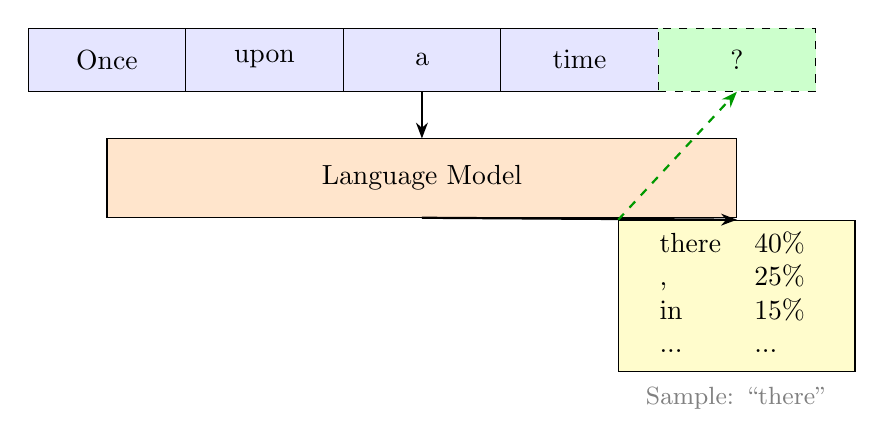
\begin{tikzpicture}[
    box/.style={rectangle, draw, minimum width=2cm, minimum height=0.8cm, align=center},
    arrow/.style={-{Stealth[length=2mm]}, thick},
]
    % Input sequence
    \node[box, fill=blue!10] (once) at (0, 0) {Once};
    \node[box, fill=blue!10] (upon) at (2, 0) {upon};
    \node[box, fill=blue!10] (a) at (4, 0) {a};
    \node[box, fill=blue!10] (time) at (6, 0) {time};
    \node[box, fill=green!20, dashed] (next) at (8, 0) {?};

    % Model
    \node[box, fill=orange!20, minimum width=8cm, minimum height=1cm] (model) at (4, -1.5) {Language Model};

    % Probabilities
    \node[box, fill=yellow!20, minimum width=3cm] (probs) at (8, -3) {
        \begin{tabular}{ll}
        there & 40\% \\
        , & 25\% \\
        in & 15\% \\
        ... & ...
        \end{tabular}
    };

    % Arrows
    \draw[arrow] (4, -0.4) -- (4, -1);
    \draw[arrow] (model.south) -- (probs.north);
    \draw[arrow, dashed, green!60!black] (probs.north west) -- (next.south);

    % Labels
    \node[font=\small, gray] at (8, -4.3) {Sample: ``there''};
\end{tikzpicture}
\caption{The autoregressive generation process. The model takes all previous tokens as input and outputs a probability distribution over possible next tokens.}
\label{fig:autoregressive}
\end{figure}

\subsection{Tokens vs. Words}

You may have noticed we use the term ``token'' rather than ``word.'' This is intentional. Modern language models don't operate on words directly---they operate on \textbf{tokens}, which are subword units.

For example, the word ``understanding'' might be split into tokens like:
\begin{lstlisting}[style=shell, numbers=none]
["under", "stand", "ing"]
\end{lstlisting}

This approach, called \textbf{subword tokenization}, offers several advantages:
\begin{itemize}
    \item Handles rare and unknown words gracefully
    \item Keeps vocabulary size manageable
    \item Works across languages
\end{itemize}

We'll explore tokenization in depth in \cref{ch:tokenization}.

% -----------------------------------------------------------------------------
\section{Training vs. Inference}
% -----------------------------------------------------------------------------

Language models have two distinct modes of operation:

\subsection{Training (Learning)}

During training, the model learns to predict the next token by observing millions of text examples. For each position in a text sequence, the model:
\begin{enumerate}
    \item Sees all tokens up to that position
    \item Predicts the next token
    \item Compares its prediction to the actual next token
    \item Adjusts its parameters to improve future predictions
\end{enumerate}

The key insight is that training data provides ``free supervision''---we don't need humans to label each example because the next word in any text serves as the label.

\begin{keypoint}
Language model training is \textbf{self-supervised}: the training signal comes from the text itself, not from human annotations. This allows training on massive amounts of unlabeled text.
\end{keypoint}

\subsection{Inference (Generation)}

During inference, we use the trained model to generate new text. The model applies what it learned during training to produce coherent continuations of any given prompt.

% -----------------------------------------------------------------------------
\section{Model Sizes: From TryLM to GPT-4}
% -----------------------------------------------------------------------------

Language models come in vastly different sizes, typically measured by their parameter count:

\begin{table}[H]
\centering
\begin{tabular}{lrl}
\toprule
\textbf{Model} & \textbf{Parameters} & \textbf{Scale} \\
\midrule
TryLM (this book) & 10--17M & Small \\
GPT-2 Small & 124M & Medium \\
GPT-2 XL & 1.5B & Large \\
LLaMA 7B & 7B & Very Large \\
GPT-3 & 175B & Massive \\
GPT-4 & $\sim$1.8T (estimated) & Enormous \\
\bottomrule
\end{tabular}
\caption{Comparison of language model sizes. TryLM is intentionally small for educational purposes.}
\label{tab:model-sizes}
\end{table}

\subsection{Why Start Small?}

You might wonder: if bigger models are more capable, why build a small one?

\begin{enumerate}
    \item \textbf{Understanding}: Small models let you see every component clearly without being overwhelmed by scale.

    \item \textbf{Iteration Speed}: Training a 10M parameter model takes hours, not weeks. You can experiment and learn quickly.

    \item \textbf{Hardware Accessibility}: You can train TryLM on a single consumer GPU (or even CPU, slowly).

    \item \textbf{Same Architecture}: TryLM uses the \textit{same architectural patterns} as billion-parameter models. The principles transfer directly.
\end{enumerate}

\begin{keypoint}
A 10-million parameter model and a 10-billion parameter model differ in \textit{scale}, not in \textit{kind}. Understanding the small model gives you genuine insight into the large one.
\end{keypoint}

% -----------------------------------------------------------------------------
\section{The TinyStories Dataset}
% -----------------------------------------------------------------------------

\TryLM trains on the \textbf{TinyStories} dataset, a collection of short stories written in simple language. This dataset was specifically designed for training and studying small language models.

\subsection{Why TinyStories?}

TinyStories was created by researchers at Microsoft who asked: \textit{``How small can a language model be and still produce coherent, grammatical text?''}

Key properties of TinyStories:
\begin{itemize}
    \item \textbf{Simple vocabulary}: Uses words that a 3--4 year old would understand
    \item \textbf{Short stories}: Each story is a few paragraphs long
    \item \textbf{Consistent structure}: Stories follow narrative patterns (beginning, middle, end)
    \item \textbf{Clean data}: Synthetically generated by GPT-3.5/4, so it's grammatically correct
\end{itemize}

\subsection{Example Story}

Here's a typical TinyStories example:

\begin{quote}
\textit{Once upon a time, there was a little girl named Lily. She loved to play in the garden with her dog, Max. One sunny day, Lily found a beautiful red flower.}

\textit{``Look, Max!'' she said. ``Isn't it pretty?''}

\textit{Max wagged his tail. Lily picked the flower and gave it to her mom. Her mom smiled and said, ``Thank you, Lily. You are so kind.''}

\textit{Lily felt happy. She learned that sharing makes everyone smile.}
\end{quote}

\subsection{Training on TinyStories}

When you train \TryLM on this dataset, the model learns:
\begin{itemize}
    \item Basic grammar and sentence structure
    \item Common narrative patterns (``Once upon a time...'')
    \item Character names and relationships
    \item Simple cause-and-effect reasoning
    \item Story conclusions and morals
\end{itemize}

After training, you can prompt the model with ``Once upon a time'' and it will generate its own coherent (if simple) stories.

% -----------------------------------------------------------------------------
\section{Modern Transformer Architecture}
% -----------------------------------------------------------------------------

\TryLM is built on the \textbf{Transformer architecture}, the dominant architecture for language models since 2017. We'll cover the transformer in detail in Part II, but here's a preview of what makes it special.

\subsection{Key Innovations}

The transformer introduced several breakthrough ideas:

\begin{enumerate}
    \item \textbf{Self-Attention}: The ability to look at all other positions in the input when processing each position. This allows the model to capture long-range dependencies.

    \item \textbf{Parallelization}: Unlike previous sequential models (RNNs), transformers can process all positions simultaneously during training, making them much faster.

    \item \textbf{Scalability}: Transformers scale remarkably well---performance continues to improve as we add more parameters and data.
\end{enumerate}

\subsection{TryLM's Architecture}

\TryLM uses a \textbf{decoder-only} transformer (the ``GPT style''), which is optimized for text generation. It incorporates several modern improvements over the original transformer:

\begin{table}[H]
\centering
\begin{tabular}{ll}
\toprule
\textbf{Component} & \textbf{Modern Choice} \\
\midrule
Normalization & RMSNorm (instead of LayerNorm) \\
Position Encoding & RoPE (instead of learned embeddings) \\
Activation & SwiGLU (instead of GELU/ReLU) \\
Norm Placement & Pre-norm (instead of post-norm) \\
\bottomrule
\end{tabular}
\caption{Modern architectural choices used in TryLM}
\label{tab:architecture-choices}
\end{table}

We'll explain why each of these choices was made in \cref{ch:design-choices}.

% -----------------------------------------------------------------------------
\section{What You'll Build}
% -----------------------------------------------------------------------------

Over the course of this book, you'll understand every component of a working language model:

\begin{figure}[H]
\centering
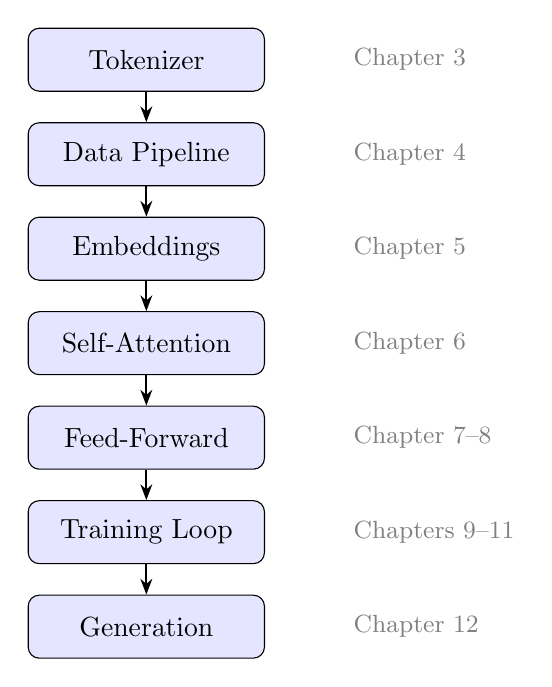
\begin{tikzpicture}[
    box/.style={rectangle, draw, rounded corners, minimum width=3cm, minimum height=0.8cm, align=center, fill=blue!10},
    arrow/.style={-{Stealth[length=2mm]}, thick},
]
    % Components
    \node[box] (tok) at (0, 0) {Tokenizer};
    \node[box] (data) at (0, -1.2) {Data Pipeline};
    \node[box] (emb) at (0, -2.4) {Embeddings};
    \node[box] (attn) at (0, -3.6) {Self-Attention};
    \node[box] (ffn) at (0, -4.8) {Feed-Forward};
    \node[box] (train) at (0, -6) {Training Loop};
    \node[box] (gen) at (0, -7.2) {Generation};

    % Chapters
    \node[right=1cm of tok, font=\small, gray] {Chapter 3};
    \node[right=1cm of data, font=\small, gray] {Chapter 4};
    \node[right=1cm of emb, font=\small, gray] {Chapter 5};
    \node[right=1cm of attn, font=\small, gray] {Chapter 6};
    \node[right=1cm of ffn, font=\small, gray] {Chapter 7--8};
    \node[right=1cm of train, font=\small, gray] {Chapters 9--11};
    \node[right=1cm of gen, font=\small, gray] {Chapter 12};

    % Arrows
    \draw[arrow] (tok) -- (data);
    \draw[arrow] (data) -- (emb);
    \draw[arrow] (emb) -- (attn);
    \draw[arrow] (attn) -- (ffn);
    \draw[arrow] (ffn) -- (train);
    \draw[arrow] (train) -- (gen);
\end{tikzpicture}
\caption{The components you'll build throughout this book}
\label{fig:components}
\end{figure}

% -----------------------------------------------------------------------------
\section{Exercises}
% -----------------------------------------------------------------------------

\begin{exercise}
\textbf{Explore Language Model Behavior}

Go to any public LLM interface (e.g., ChatGPT, Claude) and observe the generation process:
\begin{enumerate}
    \item Notice how text appears token by token
    \item Try the same prompt multiple times---do you get identical responses?
    \item What does this tell you about the probabilistic nature of language models?
\end{enumerate}
\end{exercise}

\begin{exercise}
\textbf{Thought Experiment}

Consider a language model trained only on TinyStories (simple children's stories). What tasks would this model likely be able to do? What would it fail at? Write down your predictions and revisit them after training your own model.
\end{exercise}

\begin{exercise}
\textbf{Probability Intuition}

Given the sentence ``The dog chased the...'', list 5 possible next words and estimate their probabilities. How would these probabilities change if the context was ``The cat chased the...''?
\end{exercise}

% -----------------------------------------------------------------------------
\section{Summary}
% -----------------------------------------------------------------------------

\begin{summary}
    \item A \textbf{language model} predicts the next token given previous tokens
    \item \textbf{Autoregressive generation} produces text one token at a time
    \item Training is \textbf{self-supervised}---no manual labels needed
    \item \TryLM is small (10--17M parameters) but uses \textbf{modern architectural patterns}
    \item The \textbf{TinyStories} dataset is ideal for learning due to its simple, consistent structure
    \item Understanding small models provides genuine insight into larger ones
\end{summary}

In the next chapter, we'll set up your development environment and explore the \TryLM codebase structure.

% =============================================================================
% Chapter 2: Environment Setup
% =============================================================================
\chapter{Environment Setup}
\label{ch:environment-setup}

\begin{objectives}
    \item Install Python and the \texttt{uv} package manager
    \item Clone and set up the TryLM repository
    \item Understand the project structure
    \item Run basic CLI commands
    \item (Optional) Configure GPU acceleration
\end{objectives}

% -----------------------------------------------------------------------------
\section{Prerequisites}
% -----------------------------------------------------------------------------

Before we begin, ensure you have:

\begin{itemize}
    \item A computer running Linux, macOS, or Windows (with WSL2)
    \item Python 3.11 or later
    \item Basic familiarity with the command line
    \item (Optional) An NVIDIA GPU with CUDA support for faster training
\end{itemize}

% -----------------------------------------------------------------------------
\section{Installing the uv Package Manager}
% -----------------------------------------------------------------------------

\TryLM uses \texttt{uv}, a modern, fast Python package manager written in Rust. It replaces traditional tools like \texttt{pip} and \texttt{virtualenv} with a single, unified tool.

\subsection{Why uv?}

\begin{itemize}
    \item \textbf{Speed}: 10--100x faster than pip
    \item \textbf{Reliability}: Deterministic dependency resolution
    \item \textbf{Simplicity}: Single tool for environments and packages
\end{itemize}

\subsection{Installation}

Install \texttt{uv} using the official installer:

\begin{lstlisting}[style=shell]
# Linux/macOS
curl -LsSf https://astral.sh/uv/install.sh | sh

# Windows (PowerShell)
powershell -c "irm https://astral.sh/uv/install.ps1 | iex"
\end{lstlisting}

After installation, restart your terminal and verify:

\begin{lstlisting}[style=shell]
uv --version
# uv 0.4.x
\end{lstlisting}

% -----------------------------------------------------------------------------
\section{Getting the TryLM Code}
% -----------------------------------------------------------------------------

\subsection{Clone the Repository}

\begin{lstlisting}[style=shell]
git clone https://github.com/your-repo/trylm.git
cd trylm
\end{lstlisting}

\subsection{Install Dependencies}

Use \texttt{uv} to create a virtual environment and install all dependencies:

\begin{lstlisting}[style=shell]
uv sync
\end{lstlisting}

This command:
\begin{enumerate}
    \item Creates a \texttt{.venv} virtual environment
    \item Reads \texttt{pyproject.toml} for dependency specifications
    \item Installs all required packages
\end{enumerate}

\begin{note}
All \TryLM commands use \texttt{uv run} to execute within the virtual environment. You don't need to manually activate the environment.
\end{note}

% -----------------------------------------------------------------------------
\section{Project Structure}
% -----------------------------------------------------------------------------

Let's explore the \TryLM codebase:

\begin{lstlisting}[style=shell, numbers=none]
trylm/
|-- pyproject.toml        # Project configuration and dependencies
|-- configs/
|   `-- tiny_stories.yaml # Default training configuration
|-- src/
|   `-- trylm/
|       |-- __init__.py   # Package init
|       |-- cli.py        # Command-line interface
|       |-- config.py     # Configuration dataclasses
|       |-- model.py      # GPT model architecture
|       |-- tokenizer.py  # BPE tokenizer
|       |-- data.py       # Dataset and dataloaders
|       |-- trainer.py    # Training loop
|       |-- generate.py   # Text generation
|       `-- evaluate.py   # Evaluation metrics
|-- data/                 # Tokenizer and cached data
|-- checkpoints/          # Saved model checkpoints
`-- notebooks/            # Jupyter notebooks
\end{lstlisting}

\subsection{Key Files}

\begin{table}[H]
\centering
\begin{tabular}{lp{8cm}}
\toprule
\textbf{File} & \textbf{Purpose} \\
\midrule
\texttt{model.py} & The GPT model: embeddings, attention, feed-forward layers, and the complete architecture \\
\texttt{tokenizer.py} & BPE tokenizer training and text encoding/decoding \\
\texttt{data.py} & Dataset loading, tokenization, and batch preparation \\
\texttt{trainer.py} & Training loop with optimization, checkpointing, and logging \\
\texttt{generate.py} & Text generation with various sampling strategies \\
\texttt{config.py} & Configuration dataclasses for tokenizer, model, and training \\
\texttt{cli.py} & Typer-based command-line interface \\
\bottomrule
\end{tabular}
\caption{Key source files in the TryLM project}
\end{table}

% -----------------------------------------------------------------------------
\section{The Command-Line Interface}
% -----------------------------------------------------------------------------

\TryLM provides a command-line interface (CLI) for all operations. The entry point is the \texttt{trylm} command.

\subsection{Available Commands}

\begin{lstlisting}[style=shell]
uv run trylm --help
\end{lstlisting}

This shows:
\begin{lstlisting}[style=shell, numbers=none]
Usage: trylm [OPTIONS] COMMAND [ARGS]...

Commands:
  tokenizer  Tokenizer training and encoding
  train      Train the language model
  generate   Generate text from a trained model
  eval       Evaluate model perplexity
  info       Display model information
  init       Initialize a configuration file
\end{lstlisting}

\subsection{Your First Command}

Let's check the default model configuration:

\begin{lstlisting}[style=shell]
uv run trylm info
\end{lstlisting}

Output:
\begin{lstlisting}[style=shell, numbers=none]
TryLM Model Configuration
==========================
Vocabulary size:  16,384
Context length:   512
Model dimension:  384
Attention heads:  6
Layers:           6
FFN dimension:    1,536

Estimated parameters: ~10.8M
\end{lstlisting}

\begin{keypoint}
The \texttt{trylm info} command shows the model architecture without loading any weights. It's useful for understanding the configuration before training.
\end{keypoint}

% -----------------------------------------------------------------------------
\section{Configuration System}
% -----------------------------------------------------------------------------

\TryLM uses a hierarchical configuration system defined in \texttt{config.py}.

\subsection{Configuration Dataclasses}

Three dataclasses define the complete configuration:

\begin{lstlisting}[style=python, caption={Configuration structure from config.py}]
@dataclass
class TokenizerConfig:
    vocab_size: int = 16384
    min_frequency: int = 2
    special_tokens: list[str] = field(default_factory=lambda: [
        "<|pad|>", "<|eos|>", "<|bos|>", "<|unk|>"
    ])
    save_path: Path = Path("data/tokenizer")

@dataclass
class ModelConfig:
    vocab_size: int = 16384
    n_layers: int = 6
    n_heads: int = 6
    d_model: int = 384
    d_ff: int = 1536
    context_length: int = 512
    dropout: float = 0.1
    bias: bool = False

@dataclass
class TrainConfig:
    batch_size: int = 64
    learning_rate: float = 3e-4
    max_steps: int = 10000
    # ... more options
\end{lstlisting}

\subsection{YAML Configuration Files}

Configuration can be loaded from YAML files. Here's the default \texttt{tiny\_stories.yaml}:

\begin{lstlisting}[style=yaml, caption={configs/tiny\_stories.yaml}]
tokenizer:
  vocab_size: 16384
  min_frequency: 2

model:
  vocab_size: 16384
  n_layers: 6
  n_heads: 6
  d_model: 384
  d_ff: 1536
  context_length: 512
  dropout: 0.1
  bias: false

train:
  dataset_name: roneneldan/TinyStories
  batch_size: 64
  gradient_accumulation_steps: 4
  learning_rate: 0.0003
  max_steps: 10000
  warmup_steps: 100
  eval_interval: 500
  checkpoint_dir: checkpoints
  mixed_precision: true
  compile: true
  seed: 42
\end{lstlisting}

\subsection{CLI Overrides}

Any configuration value can be overridden via command-line arguments:

\begin{lstlisting}[style=shell]
# Use config file with overrides
uv run trylm train --config configs/tiny_stories.yaml \
    --batch-size 32 \
    --max-steps 5000
\end{lstlisting}

% -----------------------------------------------------------------------------
\section{Quick Test: Training the Tokenizer}
% -----------------------------------------------------------------------------

Let's verify everything works by training a tokenizer:

\begin{lstlisting}[style=shell]
uv run trylm tokenizer train --vocab-size 16384
\end{lstlisting}

This command:
\begin{enumerate}
    \item Downloads the TinyStories dataset (first time only)
    \item Trains a BPE tokenizer on the text
    \item Saves the tokenizer to \texttt{data/tokenizer/}
\end{enumerate}

Expected output:
\begin{lstlisting}[style=shell, numbers=none]
Training tokenizer on roneneldan/TinyStories...
Processing 2,119,719 examples...
Training BPE tokenizer with vocab_size=16384...
Tokenizer saved to data/tokenizer
\end{lstlisting}

Now test encoding some text:

\begin{lstlisting}[style=shell]
uv run trylm tokenizer encode "Once upon a time"
\end{lstlisting}

Output:
\begin{lstlisting}[style=shell, numbers=none]
Text: Once upon a time
Token IDs: [1, 4521, 2378, 263, 1159, 2]
Tokens: ['<|bos|>', 'Once', ' upon', ' a', ' time', '<|eos|>']
\end{lstlisting}

% -----------------------------------------------------------------------------
\section{GPU Setup (Optional)}
% -----------------------------------------------------------------------------

Training is significantly faster on a GPU. \TryLM automatically detects and uses available GPUs.

\subsection{NVIDIA CUDA}

For NVIDIA GPUs, ensure you have:
\begin{enumerate}
    \item NVIDIA driver installed
    \item CUDA toolkit 11.8 or later
    \item cuDNN library
\end{enumerate}

Verify CUDA availability in Python:

\begin{lstlisting}[style=python]
import torch
print(torch.cuda.is_available())  # True
print(torch.cuda.get_device_name(0))  # e.g., "NVIDIA GeForce RTX 3080"
\end{lstlisting}

\subsection{Apple Silicon (MPS)}

On Apple Silicon Macs (M1/M2/M3), PyTorch uses the Metal Performance Shaders (MPS) backend:

\begin{lstlisting}[style=python]
import torch
print(torch.backends.mps.is_available())  # True on Apple Silicon
\end{lstlisting}

\subsection{Device Selection}

\TryLM automatically selects the best available device:

\begin{lstlisting}[style=python, caption={Device selection from cli.py}]
def get_device() -> str:
    if torch.cuda.is_available():
        return "cuda"
    elif torch.backends.mps.is_available():
        return "mps"
    return "cpu"
\end{lstlisting}

\begin{note}
Training on CPU is possible but slow. A 10M parameter model takes:
\begin{itemize}
    \item GPU (RTX 3080): $\sim$1 hour for 10k steps
    \item CPU (modern): $\sim$10+ hours for 10k steps
\end{itemize}
\end{note}

% -----------------------------------------------------------------------------
\section{Weights \& Biases Setup (Optional)}
% -----------------------------------------------------------------------------

\TryLM integrates with Weights \& Biases (W\&B) for experiment tracking.

\subsection{Create an Account}

Sign up at \url{https://wandb.ai} (free for personal use).

\subsection{Login}

\begin{lstlisting}[style=shell]
uv run wandb login
\end{lstlisting}

This prompts you to enter your API key.

\subsection{Verify}

When you train with W\&B enabled, you'll see:
\begin{lstlisting}[style=shell, numbers=none]
wandb: Syncing run trylm-tiny-stories
wandb: View project at https://wandb.ai/your-username/trylm
\end{lstlisting}

W\&B provides:
\begin{itemize}
    \item Real-time loss and metric plots
    \item Hyperparameter tracking
    \item Model checkpoint versioning
    \item Experiment comparison
\end{itemize}

% -----------------------------------------------------------------------------
\section{Development Tools}
% -----------------------------------------------------------------------------

For exploring and modifying the code, we recommend:

\subsection{IDE/Editor}

\begin{itemize}
    \item \textbf{VS Code} with Python extension
    \item \textbf{PyCharm} (Community or Professional)
    \item \textbf{Neovim} with LSP support
\end{itemize}

\subsection{Useful Commands}

\begin{lstlisting}[style=shell]
# Run type checking
uv run mypy src/trylm

# Run tests (if available)
uv run pytest

# Format code
uv run ruff format src/

# Lint code
uv run ruff check src/
\end{lstlisting}

% -----------------------------------------------------------------------------
\section{Troubleshooting}
% -----------------------------------------------------------------------------

\begin{pitfall}[title=Common Issues]
\textbf{``Command not found: uv''}

Ensure \texttt{uv} is in your PATH. Restart your terminal after installation.

\textbf{``CUDA out of memory''}

Reduce batch size: \texttt{--batch-size 16} or disable mixed precision.

\textbf{``Module not found: trylm''}

Run \texttt{uv sync} to install the package in development mode.

\textbf{Slow download of TinyStories}

The dataset is $\sim$500MB. First download may take several minutes.
\end{pitfall}

% -----------------------------------------------------------------------------
\section{Exercises}
% -----------------------------------------------------------------------------

\begin{exercise}
\textbf{Explore the CLI}

Run each of these commands and observe the output:
\begin{lstlisting}[style=shell, numbers=none]
uv run trylm --help
uv run trylm tokenizer --help
uv run trylm train --help
uv run trylm generate --help
\end{lstlisting}
What options are available for each command?
\end{exercise}

\begin{exercise}
\textbf{Examine the Project Structure}

Open \texttt{src/trylm/model.py} and identify:
\begin{enumerate}
    \item The main model class
    \item The attention mechanism class
    \item The feed-forward network class
\end{enumerate}
Don't worry about understanding the code yet---just get familiar with the structure.
\end{exercise}

\begin{exercise}
\textbf{Configuration Exploration}

Create a custom configuration file:
\begin{lstlisting}[style=shell, numbers=none]
uv run trylm init --output my_config.yaml
\end{lstlisting}
Open the file and identify:
\begin{enumerate}
    \item How many transformer layers are configured?
    \item What is the vocabulary size?
    \item What is the learning rate?
\end{enumerate}
\end{exercise}

% -----------------------------------------------------------------------------
\section{Summary}
% -----------------------------------------------------------------------------

\begin{summary}
    \item \texttt{uv} is a fast, modern Python package manager
    \item All commands use \texttt{uv run trylm <command>}
    \item The project follows a clean \texttt{src/} layout with separate modules for each concern
    \item Configuration uses dataclasses and YAML files
    \item CLI arguments can override configuration values
    \item GPU acceleration is automatic when available
    \item W\&B provides optional experiment tracking
\end{summary}

In the next chapter, we'll dive into tokenization---the critical first step in processing text for language models.

% =============================================================================
% Chapter 3: Tokenization
% =============================================================================
\chapter{Tokenization}
\label{ch:tokenization}

\begin{objectives}
    \item Understand why tokenization is necessary
    \item Learn how Byte Pair Encoding (BPE) works
    \item Train a tokenizer on real data
    \item Encode and decode text
    \item Understand special tokens and their purposes
\end{objectives}

% -----------------------------------------------------------------------------
\section{Why Tokenization?}
% -----------------------------------------------------------------------------

Neural networks operate on numbers, not text. Before we can feed text into a language model, we need to convert it into a sequence of integers. This process is called \textbf{tokenization}.

\begin{definition}[title=Tokenization]
\textbf{Tokenization} is the process of breaking text into discrete units (tokens) and mapping each unit to a unique integer ID.
\end{definition}

But how should we split text? There are several approaches, each with tradeoffs.

\subsection{Character-Level Tokenization}

The simplest approach: treat each character as a token.

\begin{lstlisting}[style=python]
text = "Hello"
tokens = list(text)  # ['H', 'e', 'l', 'l', 'o']
\end{lstlisting}

\textbf{Pros:}
\begin{itemize}
    \item Small vocabulary (just 256 bytes or ~65k Unicode characters)
    \item Can represent any text
\end{itemize}

\textbf{Cons:}
\begin{itemize}
    \item Very long sequences (``Hello'' becomes 5 tokens)
    \item Hard for the model to learn word-level patterns
\end{itemize}

\subsection{Word-Level Tokenization}

Split on whitespace and punctuation.

\begin{lstlisting}[style=python]
text = "Hello, world!"
tokens = ["Hello", ",", "world", "!"]
\end{lstlisting}

\textbf{Pros:}
\begin{itemize}
    \item Linguistically meaningful units
    \item Shorter sequences
\end{itemize}

\textbf{Cons:}
\begin{itemize}
    \item Huge vocabulary needed (English has 170k+ words)
    \item Cannot handle unknown words
    \item Doesn't work well across languages
\end{itemize}

\subsection{Subword Tokenization: The Best of Both Worlds}

Modern language models use \textbf{subword tokenization}, which splits text into units smaller than words but larger than characters.

\begin{lstlisting}[style=python]
text = "unhappiness"
tokens = ["un", "happiness"]  # or ["un", "happ", "iness"]
\end{lstlisting}

\begin{keypoint}
Subword tokenization balances vocabulary size with sequence length. Common words are single tokens; rare words are split into frequent subwords.
\end{keypoint}

\TryLM uses \textbf{Byte Pair Encoding (BPE)}, the most popular subword tokenization algorithm.

% -----------------------------------------------------------------------------
\section{Byte Pair Encoding (BPE)}
% -----------------------------------------------------------------------------

BPE was originally a data compression algorithm, adapted for NLP by Sennrich et al. (2016). It works by iteratively merging the most frequent pairs of tokens.

\subsection{The BPE Algorithm}

\begin{algorithm}[H]
\caption{Byte Pair Encoding Training}
\begin{algorithmic}[1]
\Require Training corpus, vocabulary size $V$
\State Initialize vocabulary with all individual bytes/characters
\While{vocabulary size $< V$}
    \State Count frequency of all adjacent token pairs in corpus
    \State Find the most frequent pair $(a, b)$
    \State Create new token $ab$ by merging $a$ and $b$
    \State Add $ab$ to vocabulary
    \State Replace all occurrences of $(a, b)$ with $ab$ in corpus
\EndWhile
\State \Return vocabulary and merge rules
\end{algorithmic}
\end{algorithm}

\subsection{BPE Example}

Let's trace through BPE on a toy corpus:

\begin{lstlisting}[style=shell, numbers=none]
Corpus: "low lower lowest"
Initial tokens: ['l', 'o', 'w', ' ', 'l', 'o', 'w', 'e', 'r', ' ',
                 'l', 'o', 'w', 'e', 's', 't']
\end{lstlisting}

\textbf{Iteration 1:} Most frequent pair is `(l, o)` (3 occurrences)
\begin{lstlisting}[style=shell, numbers=none]
Merge: l + o -> lo
Tokens: ['lo', 'w', ' ', 'lo', 'w', 'e', 'r', ' ', 'lo', 'w', 'e', 's', 't']
\end{lstlisting}

\textbf{Iteration 2:} Most frequent pair is `(lo, w)` (3 occurrences)
\begin{lstlisting}[style=shell, numbers=none]
Merge: lo + w -> low
Tokens: ['low', ' ', 'low', 'e', 'r', ' ', 'low', 'e', 's', 't']
\end{lstlisting}

\textbf{Iteration 3:} Most frequent pair is `(low, e)` (2 occurrences)
\begin{lstlisting}[style=shell, numbers=none]
Merge: low + e -> lowe
Tokens: ['low', ' ', 'lowe', 'r', ' ', 'lowe', 's', 't']
\end{lstlisting}

The algorithm continues until reaching the target vocabulary size.

\begin{figure}[H]
\centering
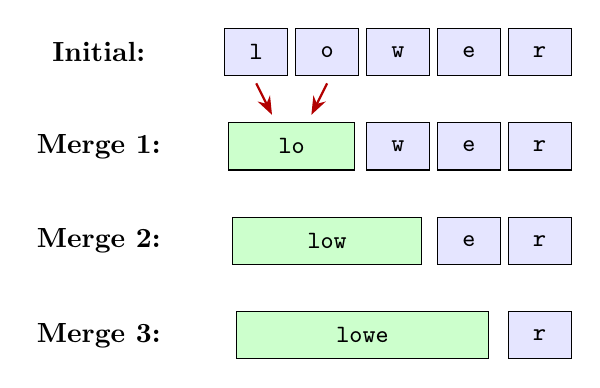
\begin{tikzpicture}[
    box/.style={rectangle, draw, minimum width=0.8cm, minimum height=0.6cm, font=\ttfamily\small},
    merge/.style={-{Stealth}, thick, red!70!black},
]
    % Initial
    \node at (-2, 0) {\textbf{Initial:}};
    \foreach \x/\c in {0/l, 0.9/o, 1.8/w, 2.7/e, 3.6/r} {
        \node[box, fill=blue!10] at (\x, 0) {\c};
    }

    % After merge 1
    \node at (-2, -1.2) {\textbf{Merge 1:}};
    \node[box, fill=green!20, minimum width=1.6cm] at (0.45, -1.2) {lo};
    \foreach \x/\c in {1.8/w, 2.7/e, 3.6/r} {
        \node[box, fill=blue!10] at (\x, -1.2) {\c};
    }
    \draw[merge] (0, -0.4) -- (0.2, -0.8);
    \draw[merge] (0.9, -0.4) -- (0.7, -0.8);

    % After merge 2
    \node at (-2, -2.4) {\textbf{Merge 2:}};
    \node[box, fill=green!20, minimum width=2.4cm] at (0.9, -2.4) {low};
    \foreach \x/\c in {2.7/e, 3.6/r} {
        \node[box, fill=blue!10] at (\x, -2.4) {\c};
    }

    % After merge 3
    \node at (-2, -3.6) {\textbf{Merge 3:}};
    \node[box, fill=green!20, minimum width=3.2cm] at (1.35, -3.6) {lowe};
    \node[box, fill=blue!10] at (3.6, -3.6) {r};
\end{tikzpicture}
\caption{BPE merge process for the word ``lower''}
\label{fig:bpe-merges}
\end{figure}

\subsection{Byte-Level BPE}

\TryLM uses \textbf{byte-level BPE}, which operates on raw bytes rather than characters. This has important advantages:

\begin{itemize}
    \item \textbf{Universal}: Can tokenize any text in any language
    \item \textbf{No unknown tokens}: Every byte sequence can be represented
    \item \textbf{Compact base vocabulary}: Only 256 base tokens (one per byte)
\end{itemize}

% -----------------------------------------------------------------------------
\section{Special Tokens}
% -----------------------------------------------------------------------------

Beyond regular text tokens, we need special tokens to mark important positions in sequences.

\subsection{The Four Special Tokens}

\TryLM uses four special tokens:

\begin{table}[H]
\centering
\begin{tabular}{lll}
\toprule
\textbf{Token} & \textbf{Name} & \textbf{Purpose} \\
\midrule
\texttt{<|bos|>} & Beginning of Sequence & Marks the start of a text \\
\texttt{<|eos|>} & End of Sequence & Marks the end of a text \\
\texttt{<|pad|>} & Padding & Fills unused positions in batches \\
\texttt{<|unk|>} & Unknown & Represents unknown tokens (rarely used) \\
\bottomrule
\end{tabular}
\caption{Special tokens in TryLM}
\label{tab:special-tokens}
\end{table}

\subsection{Why Special Tokens?}

\textbf{BOS (Beginning of Sequence):} Tells the model ``a new sequence is starting.'' During generation, we start with BOS and let the model predict what follows.

\textbf{EOS (End of Sequence):} Tells the model ``this sequence is complete.'' During generation, when the model outputs EOS, we stop generating.

\textbf{PAD (Padding):} When batching sequences of different lengths, we pad shorter ones to match the longest. PAD tokens are ignored during training.

\begin{figure}[H]
\centering
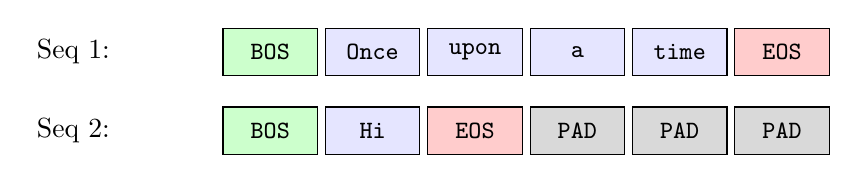
\begin{tikzpicture}[
    box/.style={rectangle, draw, minimum width=1.2cm, minimum height=0.6cm, font=\ttfamily\small},
]
    % Sequence 1
    \node at (-2.5, 0) {Seq 1:};
    \node[box, fill=green!20] at (0, 0) {BOS};
    \node[box, fill=blue!10] at (1.3, 0) {Once};
    \node[box, fill=blue!10] at (2.6, 0) {upon};
    \node[box, fill=blue!10] at (3.9, 0) {a};
    \node[box, fill=blue!10] at (5.2, 0) {time};
    \node[box, fill=red!20] at (6.5, 0) {EOS};

    % Sequence 2 (shorter, padded)
    \node at (-2.5, -1) {Seq 2:};
    \node[box, fill=green!20] at (0, -1) {BOS};
    \node[box, fill=blue!10] at (1.3, -1) {Hi};
    \node[box, fill=red!20] at (2.6, -1) {EOS};
    \node[box, fill=gray!30] at (3.9, -1) {PAD};
    \node[box, fill=gray!30] at (5.2, -1) {PAD};
    \node[box, fill=gray!30] at (6.5, -1) {PAD};
\end{tikzpicture}
\caption{Two sequences in a batch with padding}
\label{fig:special-tokens}
\end{figure}

% -----------------------------------------------------------------------------
\section{The TryLM Tokenizer}
% -----------------------------------------------------------------------------

Now let's look at how \TryLM implements tokenization. The tokenizer is built on the HuggingFace \texttt{tokenizers} library.

\subsection{Tokenizer Architecture}

\begin{lstlisting}[style=python, caption={Tokenizer training from tokenizer.py}]
@classmethod
def train(
    cls,
    texts: Iterator[str],
    config: TokenizerConfig,
    show_progress: bool = True,
) -> "TryLMTokenizer":
    """Train a new BPE tokenizer on the given texts."""
    # Initialize BPE tokenizer
    tokenizer = Tokenizer(models.BPE(unk_token=config.unk_token))

    # Set up pre-tokenization (GPT-2 style byte-level)
    tokenizer.pre_tokenizer = pre_tokenizers.ByteLevel(
        add_prefix_space=False
    )

    # Set up decoder
    tokenizer.decoder = decoders.ByteLevel()

    # Configure trainer
    trainer = trainers.BpeTrainer(
        vocab_size=config.vocab_size,
        min_frequency=config.min_frequency,
        special_tokens=config.special_tokens,
        show_progress=show_progress,
    )

    # Train the tokenizer
    tokenizer.train_from_iterator(texts, trainer=trainer)

    return cls(tokenizer, config)
\end{lstlisting}

\subsection{Key Components}

\begin{enumerate}
    \item \textbf{Model}: \texttt{BPE} --- the core tokenization algorithm
    \item \textbf{Pre-tokenizer}: \texttt{ByteLevel} --- converts text to bytes before BPE
    \item \textbf{Decoder}: \texttt{ByteLevel} --- converts bytes back to text
    \item \textbf{Trainer}: \texttt{BpeTrainer} --- learns the merge rules from data
\end{enumerate}

\subsection{Post-Processing}

After tokenization, we add special tokens automatically:

\begin{lstlisting}[style=python]
# Set up post-processor to add BOS/EOS tokens
tokenizer.post_processor = TemplateProcessing(
    single=f"{config.bos_token}:0 $A:0 {config.eos_token}:0",
    special_tokens=[
        (config.bos_token, bos_id),
        (config.eos_token, eos_id),
    ],
)
\end{lstlisting}

This means every encoded sequence automatically gets BOS at the start and EOS at the end:

\begin{lstlisting}[style=shell, numbers=none]
Input:  "Hello world"
Output: [<|bos|>, Hello, world, <|eos|>]
\end{lstlisting}

% -----------------------------------------------------------------------------
\section{Training a Tokenizer}
% -----------------------------------------------------------------------------

Let's train a tokenizer on TinyStories.

\subsection{Using the CLI}

\begin{lstlisting}[style=shell]
uv run trylm tokenizer train --vocab-size 16384
\end{lstlisting}

This:
\begin{enumerate}
    \item Loads the TinyStories dataset
    \item Trains BPE on all stories
    \item Saves the tokenizer to \texttt{data/tokenizer/}
\end{enumerate}

\subsection{Vocabulary Size Tradeoffs}

The vocabulary size is a key hyperparameter:

\begin{table}[H]
\centering
\begin{tabular}{lll}
\toprule
\textbf{Vocab Size} & \textbf{Pros} & \textbf{Cons} \\
\midrule
Small (4K) & Smaller embedding table & Longer sequences \\
Medium (16K) & Good balance & --- \\
Large (50K+) & Shorter sequences & Larger embedding table \\
\bottomrule
\end{tabular}
\caption{Vocabulary size tradeoffs}
\end{table}

\TryLM uses 16,384 tokens, which is a good balance for the TinyStories dataset.

% -----------------------------------------------------------------------------
\section{Encoding and Decoding}
% -----------------------------------------------------------------------------

Once trained, the tokenizer converts between text and token IDs.

\subsection{Encoding (Text → IDs)}

\begin{lstlisting}[style=python]
tokenizer = TryLMTokenizer.load("data/tokenizer")

text = "Once upon a time"
ids = tokenizer.encode(text)
# [1, 4521, 2378, 263, 1159, 2]
#  ^                          ^
# BOS                        EOS
\end{lstlisting}

\subsection{Decoding (IDs → Text)}

\begin{lstlisting}[style=python]
ids = [1, 4521, 2378, 263, 1159, 2]
text = tokenizer.decode(ids, skip_special_tokens=True)
# "Once upon a time"
\end{lstlisting}

\subsection{Examining Tokens}

You can see how text is split:

\begin{lstlisting}[style=shell]
uv run trylm tokenizer encode "The princess walked through the garden"
\end{lstlisting}

Output:
\begin{lstlisting}[style=shell, numbers=none]
Text: The princess walked through the garden
Tokens: 9
IDs: [1, 487, 12821, 5765, 1930, 487, 9847, 2]

Token breakdown:
  0: <|bos|> (ID: 1)
  1: The (ID: 487)
  2:  princess (ID: 12821)
  3:  walked (ID: 5765)
  4:  through (ID: 1930)
  5:  the (ID: 487)
  6:  garden (ID: 9847)
  7: <|eos|> (ID: 2)
\end{lstlisting}

\begin{note}
Notice that tokens often include leading spaces (`` princess''). This is how byte-level BPE preserves whitespace information.
\end{note}

% -----------------------------------------------------------------------------
\section{Tokenization in Practice}
% -----------------------------------------------------------------------------

\subsection{Common Patterns}

After training on TinyStories, you'll observe patterns:

\begin{itemize}
    \item Common words are single tokens: ``the'', ``said'', ``was''
    \item Less common words are split: ``beautiful'' → ``beaut'' + ``iful''
    \item Names may be split: ``Lily'' is one token; ``Bartholomew'' is several
    \item Punctuation is usually separate: ``!'' is its own token
\end{itemize}

\subsection{Batch Encoding}

For efficiency, encode multiple texts at once:

\begin{lstlisting}[style=python]
texts = ["Story one.", "Story two."]
batch_ids = tokenizer.encode_batch(texts)
# [[1, ..., 2], [1, ..., 2]]
\end{lstlisting}

% -----------------------------------------------------------------------------
\section{Common Pitfalls}
% -----------------------------------------------------------------------------

\begin{pitfall}[title=Tokenizer Mismatch]
The tokenizer must match the vocabulary size in your model configuration. If you train a tokenizer with 16K vocabulary but configure the model for 32K, you'll get errors or incorrect behavior.

Always use the same \texttt{vocab\_size} in both \texttt{TokenizerConfig} and \texttt{ModelConfig}.
\end{pitfall}

\begin{pitfall}[title=Forgetting Special Tokens]
When manually constructing token sequences, remember to include BOS and EOS tokens. The model learned with these markers---omitting them degrades performance.

\begin{lstlisting}[style=python]
# Wrong: no special tokens
ids = [4521, 2378, 263, 1159]

# Correct: includes BOS and EOS
ids = tokenizer.encode("Once upon a time")
# [1, 4521, 2378, 263, 1159, 2]
\end{lstlisting}
\end{pitfall}

\begin{pitfall}[title=Out-of-Distribution Text]
A tokenizer trained on English children's stories may poorly handle:
\begin{itemize}
    \item Code: \texttt{def foo():} might become many tokens
    \item Other languages: Chinese text will be tokenized byte-by-byte
    \item Technical jargon: ``CUDA'' might be ``C'' + ``UDA''
\end{itemize}
This is fine---the model can still process the text, just less efficiently.
\end{pitfall}

% -----------------------------------------------------------------------------
\section{Exercises}
% -----------------------------------------------------------------------------

\begin{exercise}
\textbf{Train Different Vocabulary Sizes}

Train tokenizers with different vocabulary sizes and compare:
\begin{lstlisting}[style=shell, numbers=none]
uv run trylm tokenizer train --vocab-size 8192 --output data/tok-8k
uv run trylm tokenizer train --vocab-size 32768 --output data/tok-32k
\end{lstlisting}

For the sentence ``The beautiful princess lived in a magical castle'':
\begin{enumerate}
    \item How many tokens does each tokenizer produce?
    \item Which words get split differently?
\end{enumerate}
\end{exercise}

\begin{exercise}
\textbf{Explore Token Boundaries}

Using the default tokenizer, find:
\begin{enumerate}
    \item A word that is a single token
    \item A word that gets split into exactly 2 tokens
    \item A word that gets split into 3+ tokens
\end{enumerate}

Hint: Try less common or longer words.
\end{exercise}

\begin{exercise}
\textbf{Special Token IDs}

Using Python, find the IDs of all special tokens:
\begin{lstlisting}[style=python]
from trylm.tokenizer import TryLMTokenizer

tokenizer = TryLMTokenizer.load("data/tokenizer")
print(f"BOS: {tokenizer.bos_id}")
print(f"EOS: {tokenizer.eos_id}")
print(f"PAD: {tokenizer.pad_id}")
print(f"UNK: {tokenizer.unk_id}")
\end{lstlisting}
\end{exercise}

\begin{exercise}
\textbf{Roundtrip Verification}

Verify that encode → decode is lossless:
\begin{lstlisting}[style=python]
text = "Your test sentence here!"
ids = tokenizer.encode(text)
recovered = tokenizer.decode(ids, skip_special_tokens=True)
assert text == recovered, f"Mismatch: {text!r} vs {recovered!r}"
\end{lstlisting}

Try with various texts including punctuation and numbers.
\end{exercise}

% -----------------------------------------------------------------------------
\section{Summary}
% -----------------------------------------------------------------------------

\begin{summary}
    \item \textbf{Tokenization} converts text to integers for neural network processing
    \item \textbf{BPE} (Byte Pair Encoding) is the dominant subword tokenization algorithm
    \item \textbf{Byte-level BPE} can represent any text in any language
    \item \TryLM uses four \textbf{special tokens}: BOS, EOS, PAD, UNK
    \item \textbf{Vocabulary size} balances sequence length against embedding table size
    \item Always ensure \textbf{tokenizer and model configs match}
\end{summary}

In the next chapter, we'll see how tokenized text is prepared for training as input-label pairs with padding and attention masks.

% =============================================================================
% Chapter 4: Preparing Training Data
% =============================================================================
\chapter{Preparing Training Data}
\label{ch:preparing-data}

\begin{objectives}
    \item Understand the causal language modeling objective
    \item Learn how input-target pairs are created
    \item Master padding and attention masks
    \item Implement PyTorch Datasets and DataLoaders
    \item Handle batching efficiently
\end{objectives}

% -----------------------------------------------------------------------------
\section{The Language Modeling Objective}
% -----------------------------------------------------------------------------

In \cref{ch:what-are-lms}, we learned that language models predict the next token. But how exactly do we train them to do this? The answer lies in how we structure the training data.

\subsection{Causal Language Modeling}

The training objective for GPT-style models is called \textbf{causal language modeling} (CLM). Given a sequence of tokens, the model learns to predict each token from all preceding tokens.

\begin{definition}[title=Causal Language Modeling]
For a sequence of tokens $(x_1, x_2, \ldots, x_n)$, the model learns to maximize:
\[
\mathcal{L} = \sum_{t=1}^{n} \log P(x_t | x_1, x_2, \ldots, x_{t-1})
\]
This is equivalent to minimizing the \textbf{cross-entropy loss} between predicted and actual tokens.
\end{definition}

The term ``causal'' refers to the constraint that each prediction can only depend on \textit{past} tokens---the model cannot ``peek'' at future tokens.

\subsection{Input and Target Alignment}

To train this objective, we create input-target pairs through a simple \textbf{shift operation}:

\begin{itemize}
    \item \textbf{Input}: All tokens except the last
    \item \textbf{Target}: All tokens except the first
\end{itemize}

\begin{figure}[H]
\centering
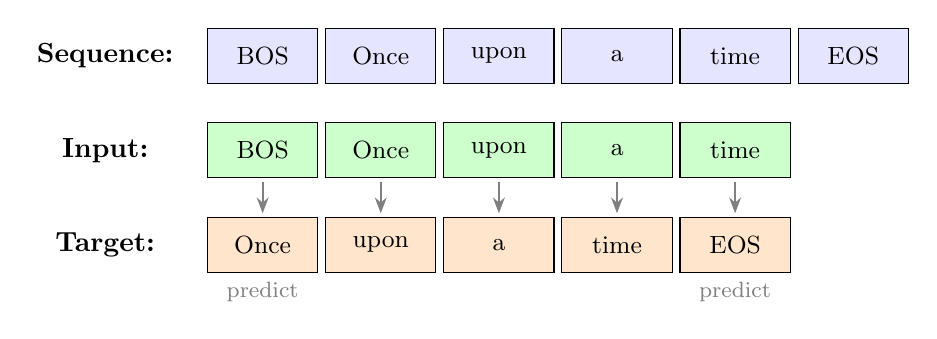
\begin{tikzpicture}[
    box/.style={rectangle, draw, minimum width=1.4cm, minimum height=0.7cm, font=\small},
    arrow/.style={-{Stealth[length=2mm]}, thick, gray},
]
    % Original sequence
    \node at (-2, 1.2) {\textbf{Sequence:}};
    \foreach \x/\t in {0/BOS, 1.5/Once, 3/upon, 4.5/a, 6/time, 7.5/EOS} {
        \node[box, fill=blue!10] at (\x, 1.2) {\t};
    }

    % Input (all but last)
    \node at (-2, 0) {\textbf{Input:}};
    \foreach \x/\t in {0/BOS, 1.5/Once, 3/upon, 4.5/a, 6/time} {
        \node[box, fill=green!20] at (\x, 0) {\t};
    }

    % Target (all but first)
    \node at (-2, -1.2) {\textbf{Target:}};
    \foreach \x/\t in {0/Once, 1.5/upon, 3/a, 4.5/time, 6/EOS} {
        \node[box, fill=orange!20] at (\x, -1.2) {\t};
    }

    % Arrows showing prediction
    \foreach \x in {0, 1.5, 3, 4.5, 6} {
        \draw[arrow] (\x, -0.4) -- (\x, -0.8);
    }

    % Labels
    \node[font=\footnotesize, gray] at (0, -1.8) {predict};
    \node[font=\footnotesize, gray] at (6, -1.8) {predict};
\end{tikzpicture}
\caption{The shift operation: input tokens predict the next token as target}
\label{fig:shift-operation}
\end{figure}

For position $i$:
\begin{itemize}
    \item The model sees \texttt{input[0:i+1]} (tokens up to and including position $i$)
    \item It predicts \texttt{target[i]} (the next token)
\end{itemize}

\begin{keypoint}
The model learns from \textbf{every position simultaneously}. A single sequence of $n$ tokens provides $n-1$ training examples (each position predicting the next token).
\end{keypoint}

% -----------------------------------------------------------------------------
\section{The TinyStories Dataset}
% -----------------------------------------------------------------------------

\TryLM trains on TinyStories, available through HuggingFace Datasets.

\subsection{Loading the Dataset}

\begin{lstlisting}[style=python]
from datasets import load_dataset

dataset = load_dataset("roneneldan/TinyStories", split="train")
print(len(dataset))  # ~2.1 million stories
print(dataset[0])
# {'text': 'One day, a little girl named Lily...'}
\end{lstlisting}

\subsection{Dataset Statistics}

\begin{table}[H]
\centering
\begin{tabular}{lr}
\toprule
\textbf{Property} & \textbf{Value} \\
\midrule
Training examples & $\sim$2.1 million \\
Validation examples & $\sim$22,000 \\
Average story length & $\sim$200 words \\
Average tokens (16K vocab) & $\sim$250 tokens \\
\bottomrule
\end{tabular}
\caption{TinyStories dataset statistics}
\end{table}

% -----------------------------------------------------------------------------
\section{Padding and Attention Masks}
% -----------------------------------------------------------------------------

Stories have different lengths. To batch them together efficiently, we need \textbf{padding}.

\subsection{The Padding Problem}

Consider two tokenized sequences:
\begin{lstlisting}[style=shell, numbers=none]
Sequence A: [BOS, Once, upon, a, time, EOS]        # 6 tokens
Sequence B: [BOS, Hi, EOS]                          # 3 tokens
\end{lstlisting}

To form a batch, both must have the same length. We pad the shorter one:
\begin{lstlisting}[style=shell, numbers=none]
Sequence A: [BOS, Once, upon, a, time, EOS]        # 6 tokens
Sequence B: [BOS, Hi, EOS, PAD, PAD, PAD]          # 6 tokens (padded)
\end{lstlisting}

\subsection{Attention Mask}

The \textbf{attention mask} tells the model which positions contain real data:

\begin{lstlisting}[style=shell, numbers=none]
Sequence B input:     [BOS, Hi, EOS, PAD, PAD, PAD]
Attention mask:       [  1,  1,   1,   0,   0,   0]
\end{lstlisting}

\begin{itemize}
    \item \textbf{1}: Real token---include in attention calculations
    \item \textbf{0}: Padding token---ignore in attention
\end{itemize}

\begin{figure}[H]
\centering
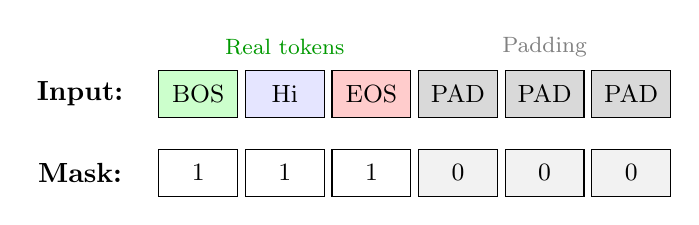
\begin{tikzpicture}[
    box/.style={rectangle, draw, minimum width=1cm, minimum height=0.6cm, font=\small},
]
    % Sequence B
    \node at (-1.5, 1) {\textbf{Input:}};
    \node[box, fill=green!20] at (0, 1) {BOS};
    \node[box, fill=blue!10] at (1.1, 1) {Hi};
    \node[box, fill=red!20] at (2.2, 1) {EOS};
    \node[box, fill=gray!30] at (3.3, 1) {PAD};
    \node[box, fill=gray!30] at (4.4, 1) {PAD};
    \node[box, fill=gray!30] at (5.5, 1) {PAD};

    % Attention mask
    \node at (-1.5, 0) {\textbf{Mask:}};
    \node[box] at (0, 0) {1};
    \node[box] at (1.1, 0) {1};
    \node[box] at (2.2, 0) {1};
    \node[box, fill=gray!10] at (3.3, 0) {0};
    \node[box, fill=gray!10] at (4.4, 0) {0};
    \node[box, fill=gray!10] at (5.5, 0) {0};

    % Labels
    \node[font=\footnotesize, green!60!black] at (1.1, 1.6) {Real tokens};
    \node[font=\footnotesize, gray] at (4.4, 1.6) {Padding};
\end{tikzpicture}
\caption{Attention mask marks real vs. padding tokens}
\label{fig:attention-mask}
\end{figure}

\subsection{Labels and the -100 Convention}

For labels (targets), we use a special convention: \textbf{-100 marks positions to ignore in the loss}.

\begin{lstlisting}[style=shell, numbers=none]
Input:   [BOS, Hi, PAD, PAD, PAD]
Labels:  [ Hi, EOS, -100, -100, -100]
\end{lstlisting}

PyTorch's \texttt{cross\_entropy} function automatically ignores positions with label -100:

\begin{lstlisting}[style=python]
import torch.nn.functional as F

# -100 positions are ignored in loss calculation
loss = F.cross_entropy(
    logits.view(-1, vocab_size),
    labels.view(-1),
    ignore_index=-100  # This is the default
)
\end{lstlisting}

\begin{keypoint}
Using -100 for padding labels ensures the model isn't penalized for predictions at padding positions---it only learns from real tokens.
\end{keypoint}

% -----------------------------------------------------------------------------
\section{The TryLM Dataset Implementation}
% -----------------------------------------------------------------------------

Let's examine how \TryLM implements the dataset.

\subsection{Dataset Class}

\begin{lstlisting}[style=python, caption={TinyStoriesDataset from data.py}]
class TinyStoriesDataset(Dataset):
    def __init__(
        self,
        tokenizer: TryLMTokenizer,
        split: str = "train",
        context_length: int = 512,
        dataset_name: str = "roneneldan/TinyStories",
    ) -> None:
        self.tokenizer = tokenizer
        self.context_length = context_length

        # Load dataset
        dataset = load_dataset(dataset_name, split=split)

        # Tokenize all texts upfront
        self.token_ids: list[list[int]] = []
        for item in dataset:
            ids = tokenizer.encode(item["text"], add_special_tokens=True)
            if len(ids) >= 2:  # Need at least 2 tokens
                self.token_ids.append(ids)

    def __len__(self) -> int:
        return len(self.token_ids)
\end{lstlisting}

\subsection{The \texttt{\_\_getitem\_\_} Method}

This is where the magic happens---creating input-target pairs:

\begin{lstlisting}[style=python, caption={Creating input-target pairs}]
def __getitem__(self, idx: int) -> dict[str, torch.Tensor]:
    ids = self.token_ids[idx]

    # Truncate if too long
    if len(ids) > self.context_length + 1:
        ids = ids[: self.context_length + 1]

    # Split into input and target (the shift operation!)
    input_ids = ids[:-1]   # All but last
    labels = ids[1:]       # All but first

    # Pad to context_length
    pad_len = self.context_length - len(input_ids)
    attention_mask = [1] * len(input_ids) + [0] * pad_len

    input_ids = input_ids + [self.tokenizer.pad_id] * pad_len
    labels = labels + [-100] * pad_len  # -100 ignored in loss

    return {
        "input_ids": torch.tensor(input_ids, dtype=torch.long),
        "labels": torch.tensor(labels, dtype=torch.long),
        "attention_mask": torch.tensor(attention_mask, dtype=torch.long),
    }
\end{lstlisting}

\subsection{Step-by-Step Example}

Let's trace through a concrete example:

\begin{lstlisting}[style=python]
# Original tokenized story (8 tokens)
ids = [1, 4521, 2378, 263, 1159, 267, 5831, 2]
#     BOS Once  upon  a    time  ,    .     EOS

# Context length = 6 (for this example)
# Need context_length + 1 = 7 tokens
# 8 > 7, so truncate:
ids = ids[:7]  # [1, 4521, 2378, 263, 1159, 267, 5831]

# Shift operation:
input_ids = ids[:-1]  # [1, 4521, 2378, 263, 1159, 267]
labels = ids[1:]      # [4521, 2378, 263, 1159, 267, 5831]

# Pad to context_length (6)
# Already length 6, so no padding needed
attention_mask = [1, 1, 1, 1, 1, 1]
\end{lstlisting}

For a shorter sequence:
\begin{lstlisting}[style=python]
# Short story (4 tokens)
ids = [1, 487, 5831, 2]  # BOS Hi . EOS

# Shift operation:
input_ids = [1, 487, 5831]     # BOS Hi .
labels = [487, 5831, 2]        # Hi . EOS

# Pad to context_length (6)
pad_len = 6 - 3 = 3

attention_mask = [1, 1, 1, 0, 0, 0]
input_ids = [1, 487, 5831, PAD, PAD, PAD]
labels = [487, 5831, 2, -100, -100, -100]
\end{lstlisting}

% -----------------------------------------------------------------------------
\section{DataLoaders and Batching}
% -----------------------------------------------------------------------------

PyTorch's \texttt{DataLoader} handles batching, shuffling, and parallel data loading.

\subsection{Creating DataLoaders}

\begin{lstlisting}[style=python, caption={DataLoader creation from data.py}]
def create_dataloaders(
    tokenizer: TryLMTokenizer,
    model_config: ModelConfig,
    train_config: TrainConfig,
) -> tuple[DataLoader, DataLoader]:

    train_dataset = TinyStoriesDataset(
        tokenizer=tokenizer,
        split=train_config.train_split,
        context_length=model_config.context_length,
    )

    train_loader = DataLoader(
        train_dataset,
        batch_size=train_config.batch_size,  # e.g., 64
        shuffle=True,          # Randomize order each epoch
        num_workers=4,         # Parallel data loading
        pin_memory=True,       # Faster GPU transfer
        drop_last=True,        # Drop incomplete final batch
    )

    return train_loader, val_loader
\end{lstlisting}

\subsection{Batch Structure}

Each batch is a dictionary of tensors:

\begin{lstlisting}[style=python]
batch = next(iter(train_loader))

print(batch["input_ids"].shape)      # [64, 512] - batch_size x context_length
print(batch["labels"].shape)         # [64, 512]
print(batch["attention_mask"].shape) # [64, 512]
\end{lstlisting}

\begin{figure}[H]
\centering
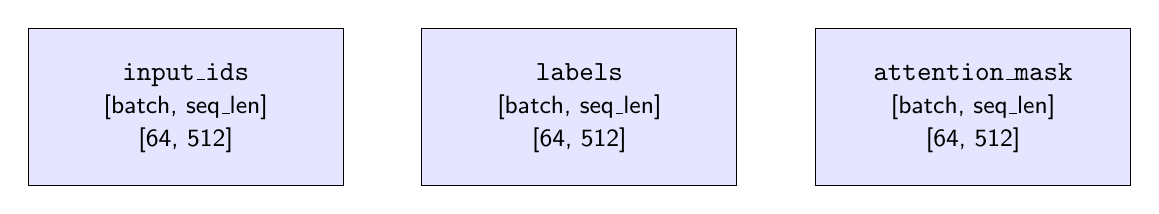
\begin{tikzpicture}[
    tensor/.style={rectangle, draw, minimum width=4cm, minimum height=2cm, fill=blue!10},
]
    \node[tensor] (input) at (0, 0) {
        \begin{tabular}{c}
        \texttt{input\_ids} \\
        \shape{batch, seq\_len} \\
        \shape{64, 512}
        \end{tabular}
    };

    \node[tensor] (labels) at (5, 0) {
        \begin{tabular}{c}
        \texttt{labels} \\
        \shape{batch, seq\_len} \\
        \shape{64, 512}
        \end{tabular}
    };

    \node[tensor] (mask) at (10, 0) {
        \begin{tabular}{c}
        \texttt{attention\_mask} \\
        \shape{batch, seq\_len} \\
        \shape{64, 512}
        \end{tabular}
    };
\end{tikzpicture}
\caption{Batch tensor shapes for batch size 64 and context length 512}
\label{fig:batch-shapes}
\end{figure}

\subsection{DataLoader Parameters Explained}

\begin{table}[H]
\centering
\begin{tabular}{lp{8cm}}
\toprule
\textbf{Parameter} & \textbf{Purpose} \\
\midrule
\texttt{batch\_size} & Number of sequences per batch (64 default) \\
\texttt{shuffle} & Randomize order each epoch (True for training) \\
\texttt{num\_workers} & Parallel processes for data loading \\
\texttt{pin\_memory} & Pre-allocate GPU memory for faster transfer \\
\texttt{drop\_last} & Drop incomplete final batch (for consistent batch sizes) \\
\bottomrule
\end{tabular}
\caption{DataLoader configuration parameters}
\end{table}

% -----------------------------------------------------------------------------
\section{Streaming Datasets}
% -----------------------------------------------------------------------------

For very large datasets, loading everything into memory may be impractical. \TryLM supports \textbf{streaming} datasets.

\subsection{Memory Comparison}

\begin{table}[H]
\centering
\begin{tabular}{lll}
\toprule
\textbf{Approach} & \textbf{Memory Usage} & \textbf{Use Case} \\
\midrule
Standard Dataset & High (all data in RAM) & Small-medium datasets \\
Streaming Dataset & Low (one batch at a time) & Large datasets \\
\bottomrule
\end{tabular}
\caption{Standard vs. streaming dataset comparison}
\end{table}

\subsection{Streaming Implementation}

\begin{lstlisting}[style=python, caption={StreamingTinyStoriesDataset from data.py}]
class StreamingTinyStoriesDataset(IterableDataset):
    def __iter__(self) -> Iterator[dict[str, torch.Tensor]]:
        dataset = load_dataset(
            self.dataset_name,
            split=self.split,
            streaming=True,  # Key difference!
        )

        if self.shuffle:
            dataset = dataset.shuffle(seed=self.seed, buffer_size=10000)

        for item in dataset:
            ids = self.tokenizer.encode(item["text"])
            # ... same processing as standard dataset
            yield {
                "input_ids": torch.tensor(input_ids),
                "labels": torch.tensor(labels),
                "attention_mask": torch.tensor(attention_mask),
            }
\end{lstlisting}

The streaming dataset loads and processes data on-the-fly, never holding the entire dataset in memory.

% -----------------------------------------------------------------------------
\section{Context Windows and Truncation}
% -----------------------------------------------------------------------------

\subsection{Why Truncate?}

The model has a fixed \textbf{context length} (512 tokens by default). Sequences longer than this must be truncated.

\begin{lstlisting}[style=python]
# If sequence is too long, truncate
if len(ids) > self.context_length + 1:
    ids = ids[: self.context_length + 1]
\end{lstlisting}

The ``+1'' accounts for the shift operation---we need \texttt{context\_length} tokens for input plus one more for the final target.

\subsection{Alternative: Chunking}

Instead of truncating long sequences, you could chunk them:

\begin{lstlisting}[style=python]
# Split long sequence into multiple training examples
def chunk_sequence(ids, context_length):
    chunks = []
    for i in range(0, len(ids) - 1, context_length):
        chunk = ids[i : i + context_length + 1]
        if len(chunk) >= 2:
            chunks.append(chunk)
    return chunks
\end{lstlisting}

\TryLM uses simple truncation, but chunking can be more data-efficient for long documents.

% -----------------------------------------------------------------------------
\section{Data Flow Summary}
% -----------------------------------------------------------------------------

\begin{figure}[H]
\centering
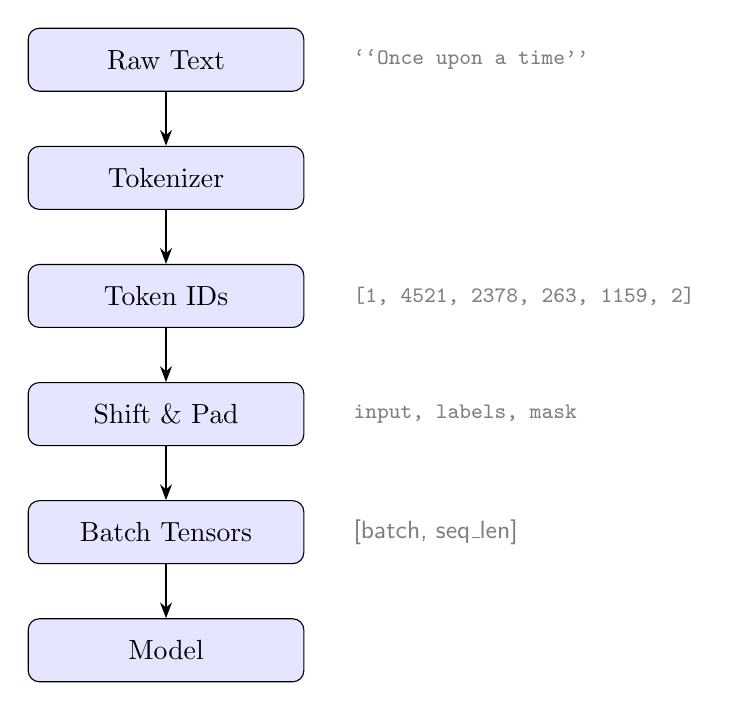
\begin{tikzpicture}[
    box/.style={rectangle, draw, rounded corners, minimum width=3.5cm, minimum height=0.8cm, align=center, fill=blue!10},
    arrow/.style={-{Stealth[length=2mm]}, thick},
    data/.style={font=\footnotesize\ttfamily, gray},
]
    % Boxes
    \node[box] (raw) at (0, 0) {Raw Text};
    \node[box] (tok) at (0, -1.5) {Tokenizer};
    \node[box] (ids) at (0, -3) {Token IDs};
    \node[box] (shift) at (0, -4.5) {Shift \& Pad};
    \node[box] (batch) at (0, -6) {Batch Tensors};
    \node[box] (model) at (0, -7.5) {Model};

    % Arrows
    \draw[arrow] (raw) -- (tok);
    \draw[arrow] (tok) -- (ids);
    \draw[arrow] (ids) -- (shift);
    \draw[arrow] (shift) -- (batch);
    \draw[arrow] (batch) -- (model);

    % Data annotations
    \node[data, right=0.5cm of raw] {``Once upon a time''};
    \node[data, right=0.5cm of ids] {[1, 4521, 2378, 263, 1159, 2]};
    \node[data, right=0.5cm of shift] {input, labels, mask};
    \node[data, right=0.5cm of batch] {\shape{batch, seq\_len}};
\end{tikzpicture}
\caption{Complete data pipeline from raw text to model input}
\label{fig:data-pipeline}
\end{figure}

% -----------------------------------------------------------------------------
\section{Common Pitfalls}
% -----------------------------------------------------------------------------

\begin{pitfall}[title=Off-by-One Errors]
The shift operation requires careful indexing:
\begin{lstlisting}[style=python]
# WRONG: input and labels have different lengths
input_ids = ids[:-1]  # n-1 tokens
labels = ids           # n tokens (mismatch!)

# CORRECT: same length, offset by 1
input_ids = ids[:-1]  # n-1 tokens
labels = ids[1:]      # n-1 tokens
\end{lstlisting}
\end{pitfall}

\begin{pitfall}[title=Forgetting -100 for Padding]
If you pad labels with 0 instead of -100, the model will try to predict the padding token:
\begin{lstlisting}[style=python]
# WRONG: model learns to predict padding tokens
labels = labels + [0] * pad_len

# CORRECT: padding positions ignored in loss
labels = labels + [-100] * pad_len
\end{lstlisting}
\end{pitfall}

\begin{pitfall}[title=Inconsistent Context Length]
The dataset must use the same context length as the model:
\begin{lstlisting}[style=python]
# These must match!
dataset = TinyStoriesDataset(context_length=512, ...)
model = GPT(ModelConfig(context_length=512))
\end{lstlisting}
\end{pitfall}

% -----------------------------------------------------------------------------
\section{Exercises}
% -----------------------------------------------------------------------------

\begin{exercise}
\textbf{Trace the Shift Operation}

Given the token sequence \texttt{[1, 100, 200, 300, 2]} with context length 4:
\begin{enumerate}
    \item What are \texttt{input\_ids}?
    \item What are \texttt{labels}?
    \item What is the \texttt{attention\_mask}?
\end{enumerate}
\end{exercise}

\begin{exercise}
\textbf{Visualize a Batch}

Load the dataset and examine a real batch:
\begin{lstlisting}[style=python, numbers=none]
from trylm.data import create_dataloaders
from trylm.tokenizer import TryLMTokenizer
from trylm.config import ModelConfig, TrainConfig

tokenizer = TryLMTokenizer.load("data/tokenizer")
train_loader, _ = create_dataloaders(
    tokenizer, ModelConfig(), TrainConfig()
)

batch = next(iter(train_loader))
print("Shapes:", {k: v.shape for k, v in batch.items()})
print("First sequence input:", batch["input_ids"][0][:20])
print("First sequence labels:", batch["labels"][0][:20])
\end{lstlisting}
\end{exercise}

\begin{exercise}
\textbf{Count Tokens}

Calculate the total number of tokens in the training set:
\begin{lstlisting}[style=python, numbers=none]
total_tokens = 0
for batch in train_loader:
    mask = batch["attention_mask"]
    total_tokens += mask.sum().item()
print(f"Total tokens: {total_tokens:,}")
\end{lstlisting}

How does this compare to the theoretical maximum (num\_examples $\times$ context\_length)?
\end{exercise}

% -----------------------------------------------------------------------------
\section{Summary}
% -----------------------------------------------------------------------------

\begin{summary}
    \item \textbf{Causal language modeling} trains models to predict the next token
    \item The \textbf{shift operation} creates input-target pairs: \texttt{input = ids[:-1]}, \texttt{target = ids[1:]}
    \item \textbf{Padding} equalizes sequence lengths for batching
    \item \textbf{Attention masks} mark real vs. padding tokens (1 vs. 0)
    \item \textbf{-100 in labels} tells PyTorch to ignore padding positions in the loss
    \item \textbf{DataLoaders} handle batching, shuffling, and parallel loading
    \item \textbf{Streaming datasets} reduce memory usage for large datasets
\end{summary}

We now have all the pieces to feed data into our model. In the next chapter, we'll begin building the model itself, starting with how token IDs become continuous vector embeddings.


% ============================================================================
% PART II: MODEL ARCHITECTURE
% ============================================================================
\part{Model Architecture}

% =============================================================================
% Chapter 5: Token Embeddings
% =============================================================================
\chapter{Token Embeddings}
\label{ch:token-embeddings}

\begin{objectives}
    \item Understand how discrete tokens become continuous vectors
    \item Learn about embedding tables and lookup operations
    \item Grasp the concept of embedding dimensions
    \item Understand weight tying between input and output embeddings
\end{objectives}

% -----------------------------------------------------------------------------
\section{From Tokens to Vectors}
% -----------------------------------------------------------------------------

In the previous chapters, we converted text to sequences of integers (token IDs). But neural networks work best with continuous values, not discrete IDs. How do we bridge this gap?

The answer is \textbf{embeddings}---learned mappings from discrete tokens to continuous vectors.

\begin{definition}[title=Token Embedding]
A \textbf{token embedding} is a dense, learned vector representation of a token. Each token ID maps to a unique vector of dimension $d_{\text{model}}$.
\end{definition}

\subsection{Why Not One-Hot Encoding?}

You might think of representing token ID 42 as a vector with 1 at position 42 and 0 everywhere else. This is called \textbf{one-hot encoding}:

\begin{lstlisting}[style=python]
vocab_size = 16384
token_id = 42

# One-hot: sparse vector with single 1
one_hot = [0, 0, ..., 1, ..., 0, 0]  # 16384-dimensional!
\end{lstlisting}

Problems with one-hot encoding:
\begin{itemize}
    \item \textbf{High dimensionality}: Vector size equals vocabulary (16,384 dimensions)
    \item \textbf{No semantic similarity}: ``cat'' and ``kitten'' are equally distant as ``cat'' and ``airplane''
    \item \textbf{Sparse}: Wastes computation on zeros
\end{itemize}

\subsection{Learned Embeddings}

Instead, we learn a \textbf{dense} representation:

\begin{lstlisting}[style=python]
d_model = 384  # Embedding dimension

# Learned embedding: dense vector
embedding = [0.23, -0.87, 0.12, ..., 0.45]  # 384-dimensional
\end{lstlisting}

Benefits:
\begin{itemize}
    \item \textbf{Low dimensionality}: 384 dimensions vs. 16,384
    \item \textbf{Semantic relationships}: Similar words have similar vectors
    \item \textbf{Dense}: Every dimension carries information
\end{itemize}

% -----------------------------------------------------------------------------
\section{The Embedding Table}
% -----------------------------------------------------------------------------

Embeddings are stored in an \textbf{embedding table} (also called an embedding matrix).

\subsection{Structure}

The table has shape \texttt{(vocab\_size, d\_model)}:

\begin{figure}[H]
\centering
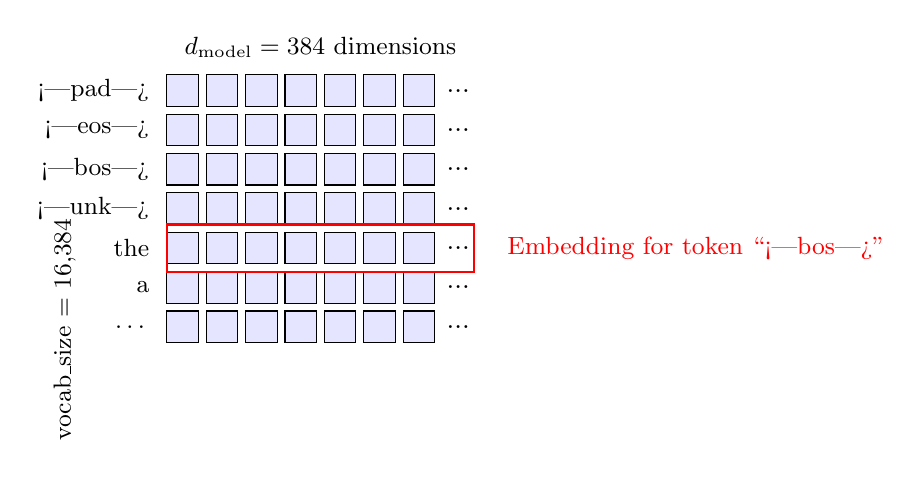
\begin{tikzpicture}[
    cell/.style={rectangle, draw, minimum width=0.4cm, minimum height=0.4cm, font=\tiny},
]
    % Draw matrix
    \foreach \y/\label in {0/<|pad|>, 1/<|eos|>, 2/<|bos|>, 3/<|unk|>, 4/the, 5/a, 6/\dots} {
        \node[left, font=\small] at (-0.3, -\y*0.5) {\label};
        \foreach \x in {0,...,7} {
            \ifnum\x=7
                \node at (\x*0.5, -\y*0.5) {...};
            \else
                \node[cell, fill=blue!10] at (\x*0.5, -\y*0.5) {};
            \fi
        }
    }

    % Labels
    \node[above, font=\small] at (1.75, 0.3) {$d_{\text{model}} = 384$ dimensions};
    \node[left, font=\small, rotate=90] at (-1.5, -1.5) {vocab\_size = 16,384};

    % Highlight one row
    \draw[thick, red] (-0.2, -2.3) rectangle (3.7, -1.7);
    \node[right, font=\small, red] at (4, -2) {Embedding for token ``<|bos|>''};
\end{tikzpicture}
\caption{The embedding table: each row is a token's learned vector representation}
\label{fig:embedding-table}
\end{figure}

\subsection{Memory Calculation}

The embedding table is often the largest part of a language model:

\begin{align*}
\text{Embedding parameters} &= \text{vocab\_size} \times d_{\text{model}} \\
&= 16,384 \times 384 \\
&= 6,291,456 \text{ parameters}
\end{align*}

At 4 bytes per float32 parameter:
\[
\text{Memory} = 6,291,456 \times 4 = 25.2 \text{ MB}
\]

\begin{keypoint}
For \TryLM, the embedding table contains $\sim$6.3 million parameters---more than half of the total $\sim$10.8 million parameters in the model!
\end{keypoint}

% -----------------------------------------------------------------------------
\section{Embedding Lookup}
% -----------------------------------------------------------------------------

The embedding operation is conceptually a \textbf{table lookup}:

\begin{lstlisting}[style=python]
import torch
import torch.nn as nn

# Create embedding table
embedding = nn.Embedding(vocab_size=16384, embedding_dim=384)

# Input: token IDs
token_ids = torch.tensor([1, 4521, 2378, 263])  # [BOS, Once, upon, a]

# Output: embeddings for each token
vectors = embedding(token_ids)
print(vectors.shape)  # torch.Size([4, 384])
\end{lstlisting}

\subsection{How It Works}

\texttt{nn.Embedding} uses the token ID as an index into the table:

\begin{lstlisting}[style=python]
# Conceptually equivalent to:
vectors = embedding.weight[token_ids]

# embedding.weight has shape [16384, 384]
# token_ids selects rows 1, 4521, 2378, 263
# Result has shape [4, 384]
\end{lstlisting}

\begin{figure}[H]
\centering
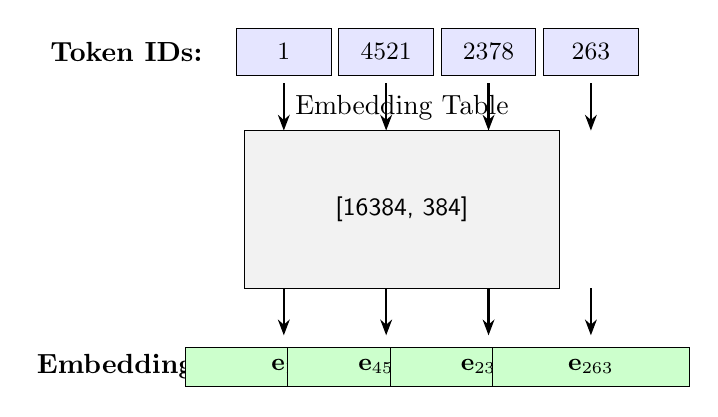
\begin{tikzpicture}[
    box/.style={rectangle, draw, minimum width=1.2cm, minimum height=0.6cm, font=\small},
    vec/.style={rectangle, draw, minimum width=2.5cm, minimum height=0.5cm, fill=green!20, font=\small},
    arrow/.style={-{Stealth[length=2mm]}, thick},
]
    % Input tokens
    \node at (-2, 2) {\textbf{Token IDs:}};
    \foreach \x/\t in {0/1, 1.3/4521, 2.6/2378, 3.9/263} {
        \node[box, fill=blue!10] at (\x, 2) {\t};
    }

    % Embedding table
    \node[rectangle, draw, minimum width=4cm, minimum height=2cm, fill=gray!10] (table) at (1.5, 0) {};
    \node[above] at (table.north) {Embedding Table};
    \node[font=\footnotesize] at (table.center) {\shape{16384, 384}};

    % Output vectors
    \node at (-2, -2) {\textbf{Embeddings:}};
    \foreach \x/\t in {0/$\mathbf{e}_1$, 1.3/$\mathbf{e}_{4521}$, 2.6/$\mathbf{e}_{2378}$, 3.9/$\mathbf{e}_{263}$} {
        \node[vec] at (\x, -2) {\t};
    }

    % Arrows
    \foreach \x in {0, 1.3, 2.6, 3.9} {
        \draw[arrow] (\x, 1.6) -- (\x, 1);
        \draw[arrow] (\x, -1) -- (\x, -1.6);
    }
\end{tikzpicture}
\caption{Embedding lookup: token IDs index into the embedding table to retrieve vectors}
\label{fig:embedding-lookup}
\end{figure}

\subsection{Batch Processing}

For a batch of sequences:

\begin{lstlisting}[style=python]
# Batch of sequences
batch = torch.tensor([
    [1, 4521, 2378, 263],   # Sequence 1
    [1, 487, 5831, 0],      # Sequence 2
])
# Shape: [2, 4] = [batch_size, seq_len]

vectors = embedding(batch)
# Shape: [2, 4, 384] = [batch_size, seq_len, d_model]
\end{lstlisting}

% -----------------------------------------------------------------------------
\section{Embeddings in TryLM}
% -----------------------------------------------------------------------------

Let's look at how \TryLM creates token embeddings:

\begin{lstlisting}[style=python, caption={Token embedding from model.py}]
class GPT(nn.Module):
    def __init__(self, config: ModelConfig) -> None:
        super().__init__()
        self.config = config

        # Token embeddings
        self.token_embedding = nn.Embedding(
            num_embeddings=config.vocab_size,  # 16384
            embedding_dim=config.d_model,      # 384
        )

        # ... rest of model
\end{lstlisting}

\subsection{In the Forward Pass}

\begin{lstlisting}[style=python, caption={Embedding lookup in forward pass}]
def forward(
    self,
    input_ids: Tensor,           # [batch, seq_len]
    attention_mask: Tensor | None = None,
    labels: Tensor | None = None,
) -> dict[str, Tensor]:

    # Convert token IDs to embeddings
    x = self.token_embedding(input_ids)  # [batch, seq_len, d_model]
    x = self.dropout(x)

    # ... pass through transformer blocks
\end{lstlisting}

% -----------------------------------------------------------------------------
\section{Weight Tying}
% -----------------------------------------------------------------------------

\TryLM uses a technique called \textbf{weight tying} (or \textbf{weight sharing}) between the input embeddings and the output projection.

\subsection{The Output Projection}

At the end of the model, we need to convert from hidden states back to vocabulary predictions:

\begin{lstlisting}[style=python]
# Hidden state: [batch, seq_len, d_model]
# We need: [batch, seq_len, vocab_size]

# Output projection (language model head)
self.lm_head = nn.Linear(
    in_features=config.d_model,      # 384
    out_features=config.vocab_size,  # 16384
    bias=False,
)
\end{lstlisting}

The \texttt{lm\_head} has shape \texttt{(vocab\_size, d\_model)}---exactly the same as the embedding table!

\subsection{Tying the Weights}

Instead of learning two separate matrices, we share them:

\begin{lstlisting}[style=python, caption={Weight tying from model.py}]
# Create embedding and output projection
self.token_embedding = nn.Embedding(config.vocab_size, config.d_model)
self.lm_head = nn.Linear(config.d_model, config.vocab_size, bias=False)

# Tie weights: lm_head uses the same matrix as token_embedding
self.lm_head.weight = self.token_embedding.weight
\end{lstlisting}

\begin{figure}[H]
\centering
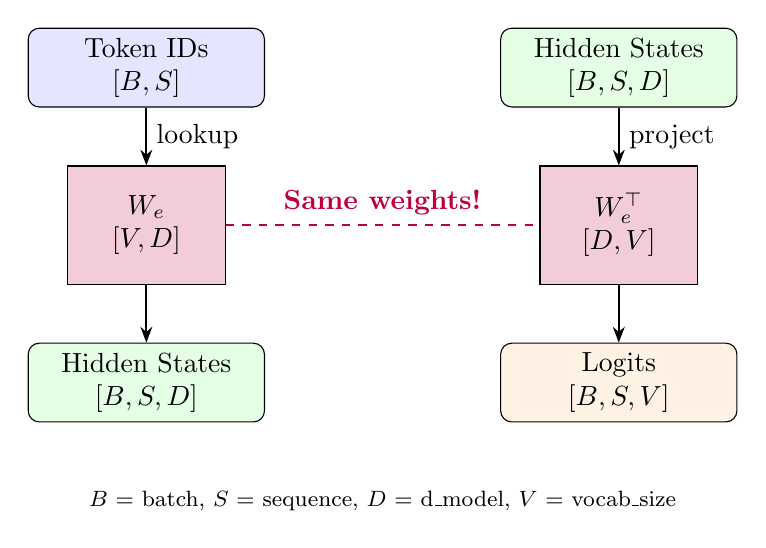
\begin{tikzpicture}[
    box/.style={rectangle, draw, rounded corners, minimum width=3cm, minimum height=1cm, align=center},
    matrix/.style={rectangle, draw, minimum width=2cm, minimum height=1.5cm, fill=purple!20, align=center},
    arrow/.style={-{Stealth[length=2mm]}, thick},
]
    % Input path
    \node[box, fill=blue!10] (input) at (0, 2) {Token IDs\\$[B, S]$};
    \node[matrix] (emb) at (0, 0) {$W_e$\\$[V, D]$};
    \node[box, fill=green!10] (hidden) at (0, -2) {Hidden States\\$[B, S, D]$};

    % Output path
    \node[box, fill=orange!10] (logits) at (6, -2) {Logits\\$[B, S, V]$};
    \node[matrix] (head) at (6, 0) {$W_e^\top$\\$[D, V]$};
    \node[box, fill=green!10] (hidden2) at (6, 2) {Hidden States\\$[B, S, D]$};

    % Arrows
    \draw[arrow] (input) -- (emb) node[midway, right] {lookup};
    \draw[arrow] (emb) -- (hidden);
    \draw[arrow] (hidden2) -- (head) node[midway, right] {project};
    \draw[arrow] (head) -- (logits);

    % Tied weights connection
    \draw[thick, dashed, purple] (emb.east) -- (head.west) node[midway, above] {\textbf{Same weights!}};

    % Legend
    \node[font=\footnotesize] at (3, -3.5) {$B$ = batch, $S$ = sequence, $D$ = d\_model, $V$ = vocab\_size};
\end{tikzpicture}
\caption{Weight tying: the same matrix is used for input embeddings and output projection}
\label{fig:weight-tying}
\end{figure}

\subsection{Why Weight Tying?}

\begin{enumerate}
    \item \textbf{Fewer parameters}: We save $16,384 \times 384 = 6.3$M parameters
    \item \textbf{Semantic consistency}: The input and output use the same token representations
    \item \textbf{Better generalization}: Empirically improves performance on language modeling
\end{enumerate}

\begin{keypoint}
Weight tying connects the token-to-vector mapping (embedding) with the vector-to-token mapping (output projection). The model must use the same representations in both directions.
\end{keypoint}

% -----------------------------------------------------------------------------
\section{What Do Embeddings Learn?}
% -----------------------------------------------------------------------------

During training, the embedding vectors are updated to capture useful properties of tokens.

\subsection{Semantic Relationships}

After training, similar words have similar embeddings:

\begin{lstlisting}[style=python]
# After training, we can measure similarity
from torch.nn.functional import cosine_similarity

dog_emb = embedding(torch.tensor([dog_id]))
cat_emb = embedding(torch.tensor([cat_id]))
car_emb = embedding(torch.tensor([car_id]))

# Similar concepts are closer
cosine_similarity(dog_emb, cat_emb)  # High (e.g., 0.8)
cosine_similarity(dog_emb, car_emb)  # Lower (e.g., 0.3)
\end{lstlisting}

\subsection{Emergent Structure}

The embedding space develops structure through training:
\begin{itemize}
    \item Words that appear in similar contexts cluster together
    \item Grammatical categories (nouns, verbs) may form regions
    \item Related concepts maintain relative positions
\end{itemize}

\subsection{Visualization}

You can visualize embeddings using dimensionality reduction:

\begin{lstlisting}[style=python]
from sklearn.manifold import TSNE
import matplotlib.pyplot as plt

# Get embeddings for some words
word_ids = [tokenizer.encode(w)[1] for w in words]  # Skip BOS
word_embs = embedding.weight[word_ids].detach().numpy()

# Reduce to 2D
tsne = TSNE(n_components=2, random_state=42)
reduced = tsne.fit_transform(word_embs)

# Plot
plt.scatter(reduced[:, 0], reduced[:, 1])
for i, word in enumerate(words):
    plt.annotate(word, reduced[i])
\end{lstlisting}

% -----------------------------------------------------------------------------
\section{Embedding Initialization}
% -----------------------------------------------------------------------------

\TryLM initializes embeddings with small random values:

\begin{lstlisting}[style=python, caption={Weight initialization from model.py}]
def _init_weights(self, module: nn.Module) -> None:
    if isinstance(module, nn.Embedding):
        torch.nn.init.normal_(module.weight, mean=0.0, std=0.02)
\end{lstlisting}

\subsection{Why This Initialization?}

\begin{itemize}
    \item \textbf{Normal distribution}: Creates diverse initial representations
    \item \textbf{Small std (0.02)}: Prevents extreme initial values
    \item \textbf{Zero mean}: No bias toward positive or negative values
\end{itemize}

This is the standard initialization used in GPT-2/3 and most modern language models.

% -----------------------------------------------------------------------------
\section{Common Pitfalls}
% -----------------------------------------------------------------------------

\begin{pitfall}[title=Forgetting to Handle Unknown Tokens]
The embedding table has a fixed vocabulary. If you encounter an out-of-vocabulary token ID, you'll get an index error:

\begin{lstlisting}[style=python]
# vocab_size = 16384
embedding(torch.tensor([99999]))  # IndexError!
\end{lstlisting}

Always use the tokenizer's UNK token for unknown inputs.
\end{pitfall}

\begin{pitfall}[title=Mismatched Vocabulary Sizes]
The embedding vocab\_size must match the tokenizer:

\begin{lstlisting}[style=python]
# WRONG: mismatch causes errors
tokenizer = TryLMTokenizer.load(...)  # vocab_size=16384
model = GPT(ModelConfig(vocab_size=32000))  # Mismatch!

# CORRECT: must match
model = GPT(ModelConfig(vocab_size=tokenizer.vocab_size))
\end{lstlisting}
\end{pitfall}

% -----------------------------------------------------------------------------
\section{Exercises}
% -----------------------------------------------------------------------------

\begin{exercise}
\textbf{Calculate Embedding Memory}

For a model with vocab\_size=50,000 and d\_model=1024:
\begin{enumerate}
    \item How many parameters are in the embedding table?
    \item How much memory (in MB) for float32?
    \item With weight tying, how much do we save?
\end{enumerate}
\end{exercise}

\begin{exercise}
\textbf{Explore Embedding Dimensions}

Experiment with different embedding dimensions:
\begin{lstlisting}[style=python, numbers=none]
for d_model in [64, 128, 256, 384, 512]:
    emb = nn.Embedding(16384, d_model)
    params = emb.weight.numel()
    print(f"d_model={d_model}: {params:,} parameters")
\end{lstlisting}

How does model quality typically change with embedding dimension?
\end{exercise}

\begin{exercise}
\textbf{Verify Weight Tying}

After creating a model, verify that weights are tied:
\begin{lstlisting}[style=python, numbers=none]
from trylm.model import GPT
from trylm.config import ModelConfig

model = GPT(ModelConfig())

# Check if weights are the same object
print(model.token_embedding.weight is model.lm_head.weight)  # True?

# Check if values are identical
print(torch.equal(model.token_embedding.weight,
                  model.lm_head.weight))  # True?
\end{lstlisting}
\end{exercise}

% -----------------------------------------------------------------------------
\section{Summary}
% -----------------------------------------------------------------------------

\begin{summary}
    \item \textbf{Embeddings} convert discrete token IDs to continuous vectors
    \item The \textbf{embedding table} has shape \texttt{(vocab\_size, d\_model)}
    \item \texttt{nn.Embedding} performs efficient \textbf{table lookup}
    \item \textbf{Weight tying} shares parameters between embedding and output projection
    \item Embeddings are \textbf{learned} during training to capture token semantics
    \item For \TryLM, embeddings account for $\sim$6M of $\sim$11M total parameters
\end{summary}

With token embeddings, we've converted token sequences into continuous representations. In the next chapter, we'll see how the model processes these embeddings using self-attention---the core mechanism that allows tokens to ``communicate'' with each other.

% =============================================================================
% Chapter 6: Self-Attention
% =============================================================================
\chapter{Self-Attention: The Heart of Transformers}
\label{ch:self-attention}

\begin{objectives}
    \item Understand the intuition behind self-attention
    \item Master Query, Key, and Value matrices
    \item Compute scaled dot-product attention step by step
    \item Understand causal masking for autoregressive models
    \item Learn multi-head attention and why it's useful
    \item Understand Rotary Position Embeddings (RoPE)
\end{objectives}

% -----------------------------------------------------------------------------
\section{The Attention Intuition}
% -----------------------------------------------------------------------------

Self-attention is the core innovation of the Transformer architecture. But what problem does it solve?

\subsection{The Challenge of Context}

Consider the sentence: ``The cat sat on the mat because \textbf{it} was tired.''

To understand what ``it'' refers to, we need to look at earlier words in the sentence. In this case, ``it'' refers to ``cat.''

Traditional sequential models (RNNs) process text one word at a time, making it hard to connect distant words. Self-attention solves this by allowing \textbf{every position to directly attend to every other position}.

\begin{keypoint}
Self-attention lets each token ``look at'' all other tokens in the sequence and decide which ones are relevant. It's like having a direct communication channel between any two positions.
\end{keypoint}

\subsection{Attention as Weighted Retrieval}

Think of attention as a soft lookup in a database:
\begin{enumerate}
    \item You have a \textbf{query}: ``What information do I need?''
    \item The database has \textbf{keys}: ``Here's what each entry is about''
    \item Each entry has a \textbf{value}: ``Here's the actual content''
    \item You compare your query to all keys, then retrieve a weighted sum of values
\end{enumerate}

% -----------------------------------------------------------------------------
\section{Query, Key, and Value}
% -----------------------------------------------------------------------------

Self-attention uses three linear projections: Query ($Q$), Key ($K$), and Value ($V$).

\subsection{The Three Projections}

Given input embeddings $X \in \mathbb{R}^{n \times d}$ (where $n$ is sequence length and $d$ is dimension):

\begin{align}
Q &= X W^Q \quad \text{(Query: ``What am I looking for?'')} \\
K &= X W^K \quad \text{(Key: ``What do I contain?'')} \\
V &= X W^V \quad \text{(Value: ``What information do I provide?'')}
\end{align}

where $W^Q, W^K, W^V \in \mathbb{R}^{d \times d}$ are learned weight matrices.

\begin{figure}[H]
\centering
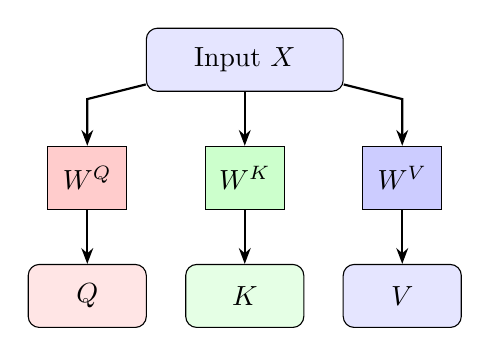
\begin{tikzpicture}[
    box/.style={rectangle, draw, rounded corners, minimum width=1.5cm, minimum height=0.8cm, fill=blue!10},
    proj/.style={rectangle, draw, minimum width=1cm, minimum height=0.8cm},
    arrow/.style={-{Stealth[length=2mm]}, thick},
]
    % Input
    \node[box, minimum width=2.5cm] (x) at (0, 0) {Input $X$};

    % Projections
    \node[proj, fill=red!20] (wq) at (-2, -1.5) {$W^Q$};
    \node[proj, fill=green!20] (wk) at (0, -1.5) {$W^K$};
    \node[proj, fill=blue!20] (wv) at (2, -1.5) {$W^V$};

    % Outputs
    \node[box, fill=red!10] (q) at (-2, -3) {$Q$};
    \node[box, fill=green!10] (k) at (0, -3) {$K$};
    \node[box, fill=blue!10] (v) at (2, -3) {$V$};

    % Arrows
    \draw[arrow] (x) -- (-2, -0.5) -- (wq);
    \draw[arrow] (x) -- (wk);
    \draw[arrow] (x) -- (2, -0.5) -- (wv);
    \draw[arrow] (wq) -- (q);
    \draw[arrow] (wk) -- (k);
    \draw[arrow] (wv) -- (v);
\end{tikzpicture}
\caption{The input is projected into three separate representations: Query, Key, and Value}
\label{fig:qkv-projection}
\end{figure}

\subsection{In TryLM's Code}

\TryLM combines Q, K, V into a single projection for efficiency:

\begin{lstlisting}[style=python, caption={QKV projection from model.py}]
class MultiHeadSelfAttention(nn.Module):
    def __init__(self, config: ModelConfig) -> None:
        super().__init__()
        self.n_heads = config.n_heads
        self.head_dim = config.d_model // config.n_heads  # 384/6 = 64

        # Combined QKV projection (more efficient than separate)
        self.qkv_proj = nn.Linear(
            config.d_model,
            3 * config.d_model,  # Q, K, V concatenated
            bias=False,
        )
\end{lstlisting}

% -----------------------------------------------------------------------------
\section{Scaled Dot-Product Attention}
% -----------------------------------------------------------------------------

The core attention computation is the \textbf{scaled dot-product attention}:

\begin{equation}
\Attention(Q, K, V) = \softmax\left(\frac{QK^\top}{\sqrt{d_k}}\right) V
\label{eq:attention}
\end{equation}

Let's break this down step by step.

\subsection{Step 1: Compute Attention Scores}

First, compute the dot product between each query and all keys:

\[
\text{scores} = Q K^\top
\]

The score between query $i$ and key $j$ measures how much position $i$ should attend to position $j$:

\begin{figure}[H]
\centering
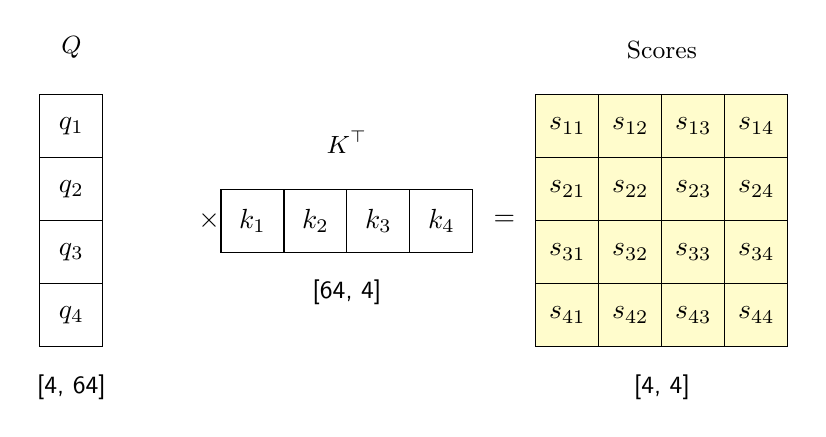
\begin{tikzpicture}[
    mat/.style={matrix of nodes, nodes={draw, minimum size=8mm, anchor=center},
                column sep=-\pgflinewidth, row sep=-\pgflinewidth},
]
    % Q matrix
    \matrix[mat] (Q) at (0, 0) {
        $q_1$ \\
        $q_2$ \\
        $q_3$ \\
        $q_4$ \\
    };
    \node[above=0.2cm of Q, font=\small] {$Q$};
    \node[below=0.1cm of Q, font=\footnotesize] {\shape{4, 64}};

    % K^T matrix
    \matrix[mat] (K) at (3.5, 0) {
        $k_1$ & $k_2$ & $k_3$ & $k_4$ \\
    };
    \node[above=0.2cm of K, font=\small] {$K^\top$};
    \node[below=0.1cm of K, font=\footnotesize] {\shape{64, 4}};

    % Scores matrix
    \matrix[mat, nodes={fill=yellow!20}] (S) at (7.5, 0) {
        $s_{11}$ & $s_{12}$ & $s_{13}$ & $s_{14}$ \\
        $s_{21}$ & $s_{22}$ & $s_{23}$ & $s_{24}$ \\
        $s_{31}$ & $s_{32}$ & $s_{33}$ & $s_{34}$ \\
        $s_{41}$ & $s_{42}$ & $s_{43}$ & $s_{44}$ \\
    };
    \node[above=0.2cm of S, font=\small] {Scores};
    \node[below=0.1cm of S, font=\footnotesize] {\shape{4, 4}};

    % Multiplication symbols
    \node at (1.75, 0) {$\times$};
    \node at (5.5, 0) {$=$};
\end{tikzpicture}
\caption{Attention scores are computed as $QK^\top$. Each cell $s_{ij}$ is the dot product of $q_i$ and $k_j$.}
\label{fig:attention-scores}
\end{figure}

\subsection{Step 2: Scale the Scores}

We divide by $\sqrt{d_k}$ (the square root of the key dimension):

\[
\text{scaled\_scores} = \frac{Q K^\top}{\sqrt{d_k}}
\]

\begin{keypoint}[title=Why Scale?]
Without scaling, dot products can become very large when $d_k$ is large. Large values cause softmax to produce near-one-hot outputs, which leads to vanishing gradients. Scaling keeps values in a reasonable range for stable training.
\end{keypoint}

For \TryLM with $d_k = 64$:
\[
\sqrt{d_k} = \sqrt{64} = 8
\]

\subsection{Step 3: Apply Softmax}

Softmax converts scores to probabilities (each row sums to 1):

\[
\text{weights} = \softmax\left(\frac{Q K^\top}{\sqrt{d_k}}\right)
\]

\begin{figure}[H]
\centering
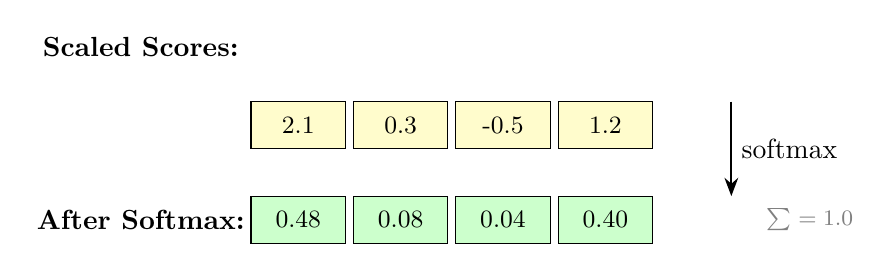
\begin{tikzpicture}[
    cell/.style={rectangle, draw, minimum width=1.2cm, minimum height=0.6cm, font=\small},
]
    % Before softmax
    \node at (-2, 1) {\textbf{Scaled Scores:}};
    \foreach \y/\vals in {0/{2.1, 0.3, -0.5, 1.2}} {
        \foreach \x/\v in {0/2.1, 1.3/0.3, 2.6/-0.5, 3.9/1.2} {
            \node[cell, fill=yellow!20] at (\x, \y) {\v};
        }
    }

    % After softmax
    \node at (-2, -1.2) {\textbf{After Softmax:}};
    \foreach \y/\vals in {0/{0.48, 0.08, 0.04, 0.40}} {
        \foreach \x/\v in {0/0.48, 1.3/0.08, 2.6/0.04, 3.9/0.40} {
            \node[cell, fill=green!20] at (\x, -1.2) {\v};
        }
    }

    % Arrow
    \draw[-{Stealth}, thick] (5.5, 0.3) -- (5.5, -0.9) node[midway, right] {softmax};

    % Sum annotation
    \node[font=\footnotesize, gray] at (6.5, -1.2) {$\sum = 1.0$};
\end{tikzpicture}
\caption{Softmax converts scores to attention weights that sum to 1}
\label{fig:softmax}
\end{figure}

\subsection{Step 4: Weighted Sum of Values}

Finally, we compute a weighted sum of the value vectors:

\[
\text{output} = \text{weights} \cdot V
\]

Each output position is a weighted combination of all value vectors, where the weights come from the attention pattern.

\subsection{Complete Example}

Let's trace through a 4-token sequence with $d_k = 64$:

\begin{lstlisting}[style=python]
# Input: [batch=1, seq=4, d_model=64]
Q = ...  # [1, 4, 64]
K = ...  # [1, 4, 64]
V = ...  # [1, 4, 64]

# Step 1: Attention scores
scores = Q @ K.transpose(-2, -1)  # [1, 4, 4]

# Step 2: Scale
scores = scores / math.sqrt(64)   # [1, 4, 4], values ~1

# Step 3: Softmax (per row)
weights = F.softmax(scores, dim=-1)  # [1, 4, 4], rows sum to 1

# Step 4: Weighted sum of values
output = weights @ V  # [1, 4, 64]
\end{lstlisting}

% -----------------------------------------------------------------------------
\section{Causal Masking}
% -----------------------------------------------------------------------------

For autoregressive language models like GPT, there's a crucial constraint: \textbf{each position can only attend to previous positions}, not future ones.

\subsection{Why Causal Masking?}

During training, we process entire sequences at once. But we want the model to learn to predict the next token using only past context. If position 3 could see position 4, it would be ``cheating''---seeing the answer it's supposed to predict!

\subsection{The Causal Mask}

We use a \textbf{lower triangular mask} to block attention to future positions:

\begin{figure}[H]
\centering
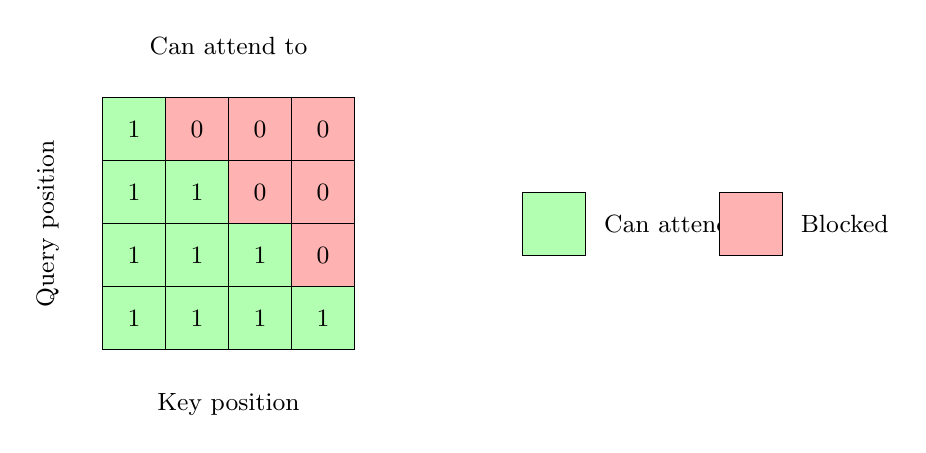
\begin{tikzpicture}[
    cell/.style={rectangle, draw, minimum size=8mm, font=\small},
]
    % Mask matrix
    \matrix[matrix of nodes, nodes={cell}, column sep=-\pgflinewidth, row sep=-\pgflinewidth] (M) {
        |[fill=green!30]| 1 & |[fill=red!30]| 0 & |[fill=red!30]| 0 & |[fill=red!30]| 0 \\
        |[fill=green!30]| 1 & |[fill=green!30]| 1 & |[fill=red!30]| 0 & |[fill=red!30]| 0 \\
        |[fill=green!30]| 1 & |[fill=green!30]| 1 & |[fill=green!30]| 1 & |[fill=red!30]| 0 \\
        |[fill=green!30]| 1 & |[fill=green!30]| 1 & |[fill=green!30]| 1 & |[fill=green!30]| 1 \\
    };

    % Labels
    \node[above=0.3cm of M, font=\small] {Can attend to};
    \node[left=0.3cm of M, font=\small, rotate=90, anchor=south] {Query position};
    \node[below=0.3cm of M, font=\small] {Key position};

    % Legend
    \node[cell, fill=green!30, right=2cm of M] (yes) {};
    \node[right=0.1cm of yes, font=\small] {Can attend};
    \node[cell, fill=red!30, right=4.5cm of M] (no) {};
    \node[right=0.1cm of no, font=\small] {Blocked};
\end{tikzpicture}
\caption{The causal mask: position $i$ can only attend to positions $\leq i$}
\label{fig:causal-mask}
\end{figure}

\subsection{Implementation}

We implement masking by setting blocked positions to $-\infty$ before softmax:

\begin{lstlisting}[style=python, caption={Causal masking from model.py}]
# Create causal mask (upper triangular = True where we should mask)
causal_mask = torch.triu(
    torch.ones(context_length, context_length, dtype=torch.bool),
    diagonal=1,
)
self.register_buffer("causal_mask", causal_mask)

# In forward pass:
scores = Q @ K.transpose(-2, -1) / math.sqrt(self.head_dim)

# Apply causal mask: set future positions to -infinity
scores = scores.masked_fill(
    self.causal_mask[:seq_len, :seq_len],
    float("-inf")
)

# Softmax converts -inf to 0
weights = F.softmax(scores, dim=-1)
\end{lstlisting}

When softmax sees $-\infty$, it outputs 0---effectively blocking attention to those positions.

% -----------------------------------------------------------------------------
\section{Multi-Head Attention}
% -----------------------------------------------------------------------------

Instead of using one large attention head, we use multiple smaller heads in parallel.

\subsection{Why Multiple Heads?}

Different heads can learn to attend to different things:
\begin{itemize}
    \item One head might focus on syntactic relationships
    \item Another might capture semantic similarity
    \item Another might track pronoun references
\end{itemize}

\subsection{How It Works}

For \TryLM with $d_{\text{model}} = 384$ and $n_{\text{heads}} = 6$:

\begin{itemize}
    \item Each head has dimension $d_k = 384 / 6 = 64$
    \item All 6 heads compute attention in parallel
    \item Outputs are concatenated back to 384 dimensions
\end{itemize}

\begin{figure}[H]
\centering
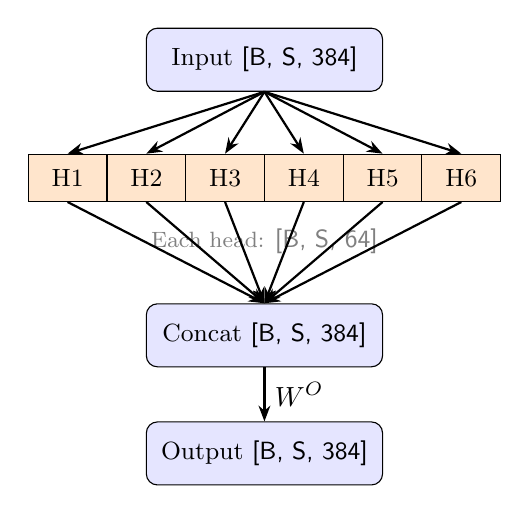
\begin{tikzpicture}[
    box/.style={rectangle, draw, rounded corners, minimum width=1.5cm, minimum height=0.8cm, fill=blue!10, font=\small},
    head/.style={rectangle, draw, minimum width=1cm, minimum height=0.6cm, font=\small},
    arrow/.style={-{Stealth[length=2mm]}, thick},
]
    % Input
    \node[box, minimum width=3cm] (input) at (0, 0) {Input \shape{B, S, 384}};

    % Heads
    \foreach \x/\h in {-2.5/1, -1.5/2, -0.5/3, 0.5/4, 1.5/5, 2.5/6} {
        \node[head, fill=orange!20] (h\h) at (\x, -1.5) {H\h};
        \draw[arrow] (input.south) -- (h\h.north);
    }
    \node[font=\footnotesize, gray] at (0, -2.3) {Each head: \shape{B, S, 64}};

    % Concat
    \node[box, minimum width=3cm] (concat) at (0, -3.5) {Concat \shape{B, S, 384}};
    \foreach \h in {1,2,3,4,5,6} {
        \draw[arrow] (h\h.south) -- (concat.north);
    }

    % Output projection
    \node[box, minimum width=3cm] (output) at (0, -5) {Output \shape{B, S, 384}};
    \draw[arrow] (concat) -- (output) node[midway, right] {$W^O$};
\end{tikzpicture}
\caption{Multi-head attention: 6 parallel attention heads, each with 64 dimensions}
\label{fig:multi-head}
\end{figure}

\subsection{Implementation}

\begin{lstlisting}[style=python, caption={Multi-head attention reshape from model.py}]
def forward(self, x: Tensor, attention_mask: Tensor | None = None) -> Tensor:
    batch_size, seq_len, _ = x.shape

    # Project to Q, K, V
    qkv = self.qkv_proj(x)  # [B, S, 3*384]

    # Reshape to [B, S, 3, n_heads, head_dim]
    qkv = qkv.view(batch_size, seq_len, 3, self.n_heads, self.head_dim)

    # Permute to [3, B, n_heads, S, head_dim]
    qkv = qkv.permute(2, 0, 3, 1, 4)

    # Separate Q, K, V
    q, k, v = qkv[0], qkv[1], qkv[2]  # Each: [B, n_heads, S, head_dim]

    # Compute attention for all heads in parallel
    # ... attention computation ...

    # Concatenate heads: [B, S, n_heads * head_dim] = [B, S, 384]
    output = output.transpose(1, 2).contiguous().view(batch_size, seq_len, -1)

    # Final output projection
    return self.out_proj(output)
\end{lstlisting}

% -----------------------------------------------------------------------------
\section{Rotary Position Embeddings (RoPE)}
% -----------------------------------------------------------------------------

Unlike the original Transformer which added position embeddings, \TryLM uses \textbf{Rotary Position Embeddings (RoPE)}---a more modern approach.

\subsection{The Problem with Learned Positions}

Traditional position embeddings:
\begin{itemize}
    \item Fixed maximum length (can't extrapolate)
    \item Absolute positions (position 5 always has the same embedding)
    \item Added to token embeddings (mixed with content)
\end{itemize}

\subsection{How RoPE Works}

RoPE encodes position through \textbf{rotation in the embedding space}:
\begin{itemize}
    \item Positions are encoded as rotation angles
    \item Applied directly to Q and K (not added to embeddings)
    \item Relative positions emerge naturally from the rotation difference
\end{itemize}

The key insight: when computing $q_m \cdot k_n$, the rotation at position $m$ and $n$ combine to give a function of $(m - n)$---the relative position!

\begin{equation}
\text{RoPE}(x, m) = x \cdot \cos(m\theta) + \text{rotate}(x) \cdot \sin(m\theta)
\end{equation}

\subsection{Implementation}

\begin{lstlisting}[style=python, caption={RoPE from model.py}]
class RotaryPositionalEmbedding(nn.Module):
    def __init__(self, dim: int, max_seq_len: int = 2048, base: float = 10000.0):
        super().__init__()
        # Precompute frequency bands
        inv_freq = 1.0 / (base ** (torch.arange(0, dim, 2).float() / dim))
        self.register_buffer("inv_freq", inv_freq)

        # Precompute cos/sin for efficiency
        self._update_cos_sin_cache(max_seq_len)

    def forward(self, x: Tensor, seq_len: int) -> tuple[Tensor, Tensor]:
        return (
            self.cos_cached[:seq_len],
            self.sin_cached[:seq_len],
        )
\end{lstlisting}

\subsection{Applying RoPE to Q and K}

\begin{lstlisting}[style=python]
def apply_rotary_pos_emb(q, k, cos, sin):
    # Rotate Q
    q_embed = (q * cos) + (rotate_half(q) * sin)

    # Rotate K
    k_embed = (k * cos) + (rotate_half(k) * sin)

    return q_embed, k_embed
\end{lstlisting}

\begin{keypoint}
RoPE advantages:
\begin{enumerate}
    \item \textbf{Relative positions}: Attention naturally depends on relative, not absolute, positions
    \item \textbf{Extrapolation}: Can handle longer sequences than seen during training
    \item \textbf{Efficiency}: Precomputed and applied with simple operations
\end{enumerate}
\end{keypoint}

% -----------------------------------------------------------------------------
\section{Putting It All Together}
% -----------------------------------------------------------------------------

Here's the complete attention flow:

\begin{enumerate}
    \item \textbf{Project} input to Q, K, V
    \item \textbf{Apply RoPE} to Q and K for position encoding
    \item \textbf{Compute scores}: $QK^\top / \sqrt{d_k}$
    \item \textbf{Apply causal mask}: block future positions
    \item \textbf{Softmax}: convert to attention weights
    \item \textbf{Apply attention mask}: zero out padding
    \item \textbf{Weighted sum}: multiply weights by V
    \item \textbf{Concatenate} heads and project output
\end{enumerate}

% -----------------------------------------------------------------------------
\section{Exercises}
% -----------------------------------------------------------------------------

\begin{exercise}
\textbf{Manual Attention Calculation}

Given:
\begin{lstlisting}[style=python, numbers=none]
Q = [[1, 0], [0, 1]]  # 2x2
K = [[1, 0], [0, 1]]  # 2x2
V = [[1, 2], [3, 4]]  # 2x2
\end{lstlisting}

Compute by hand:
\begin{enumerate}
    \item Attention scores ($QK^\top$)
    \item Scaled scores (divide by $\sqrt{2}$)
    \item Softmax of each row
    \item Final output (weights $\times$ V)
\end{enumerate}
\end{exercise}

\begin{exercise}
\textbf{Visualize Attention Patterns}

After training a model, visualize attention weights:
\begin{lstlisting}[style=python, numbers=none]
# Hook into attention layer to capture weights
# Plot as a heatmap
import matplotlib.pyplot as plt
plt.imshow(attention_weights[0, 0].detach().numpy())
plt.xlabel("Key position")
plt.ylabel("Query position")
\end{lstlisting}

What patterns do you observe? Do different heads attend differently?
\end{exercise}

% -----------------------------------------------------------------------------
\section{Summary}
% -----------------------------------------------------------------------------

\begin{summary}
    \item \textbf{Self-attention} allows each position to attend to all others
    \item \textbf{Q, K, V} are projections of the input: query (what I seek), key (what I offer), value (my content)
    \item \textbf{Scaled dot-product attention}: $\softmax(QK^\top / \sqrt{d_k}) \cdot V$
    \item \textbf{Causal masking} prevents attending to future positions (critical for autoregressive models)
    \item \textbf{Multi-head attention} runs multiple attention in parallel for richer representations
    \item \textbf{RoPE} encodes positions through rotation, enabling relative position awareness
\end{summary}

Self-attention gives the model the ability to dynamically focus on relevant context. In the next chapter, we'll combine attention with feed-forward networks to form complete transformer blocks.

% =============================================================================
% Chapter 7: Transformer Blocks
% =============================================================================
\chapter{Transformer Blocks}
\label{ch:transformer-blocks}

\begin{objectives}
    \item Understand the feed-forward network and SwiGLU activation
    \item Learn about RMSNorm and why it's preferred over LayerNorm
    \item Master the pre-normalization pattern
    \item Understand residual connections and gradient flow
    \item See how components combine into a complete transformer block
\end{objectives}

% -----------------------------------------------------------------------------
\section{Anatomy of a Transformer Block}
% -----------------------------------------------------------------------------

A transformer block combines self-attention with a feed-forward network, connected by residual connections and normalization layers.

\begin{figure}[H]
\centering
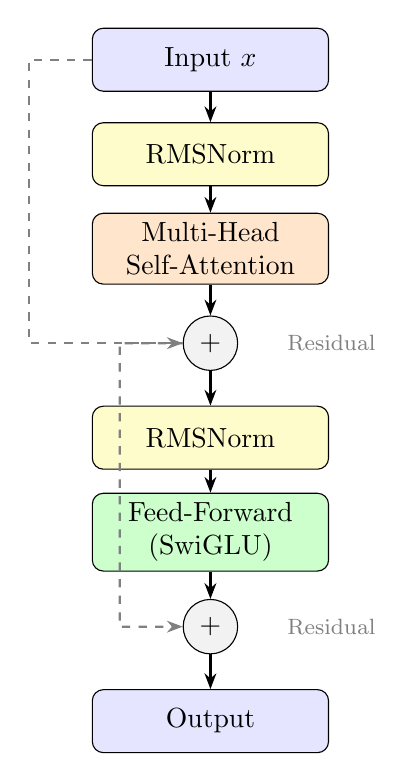
\begin{tikzpicture}[
    box/.style={rectangle, draw, rounded corners, minimum width=3cm, minimum height=0.8cm, align=center},
    norm/.style={box, fill=yellow!20},
    attn/.style={box, fill=orange!20},
    ffn/.style={box, fill=green!20},
    add/.style={circle, draw, minimum size=0.6cm, fill=gray!10},
    arrow/.style={-{Stealth[length=2mm]}, thick},
]
    % Input
    \node[box, fill=blue!10] (input) at (0, 0) {Input $x$};

    % First norm + attention
    \node[norm] (norm1) at (0, -1.2) {RMSNorm};
    \node[attn] (attn) at (0, -2.4) {Multi-Head\\Self-Attention};

    % First residual add
    \node[add] (add1) at (0, -3.6) {$+$};

    % Second norm + FFN
    \node[norm] (norm2) at (0, -4.8) {RMSNorm};
    \node[ffn] (ffn) at (0, -6) {Feed-Forward\\(SwiGLU)};

    % Second residual add
    \node[add] (add2) at (0, -7.2) {$+$};

    % Output
    \node[box, fill=blue!10] (output) at (0, -8.4) {Output};

    % Main flow
    \draw[arrow] (input) -- (norm1);
    \draw[arrow] (norm1) -- (attn);
    \draw[arrow] (attn) -- (add1);
    \draw[arrow] (add1) -- (norm2);
    \draw[arrow] (norm2) -- (ffn);
    \draw[arrow] (ffn) -- (add2);
    \draw[arrow] (add2) -- (output);

    % Residual connections
    \draw[arrow, dashed, gray] (input.west) -- ++(-0.8, 0) -- ++(0, -3.6) -- (add1.west);
    \draw[arrow, dashed, gray] (add1.west) -- ++(-0.8, 0) -- ++(0, -3.6) -- (add2.west);

    % Labels
    \node[right=0.5cm of add1, font=\footnotesize, gray] {Residual};
    \node[right=0.5cm of add2, font=\footnotesize, gray] {Residual};
\end{tikzpicture}
\caption{A complete transformer block with pre-normalization}
\label{fig:transformer-block}
\end{figure}

The block can be expressed as:
\begin{align}
x' &= x + \text{Attention}(\text{RMSNorm}(x)) \\
\text{output} &= x' + \text{FFN}(\text{RMSNorm}(x'))
\end{align}

% -----------------------------------------------------------------------------
\section{RMSNorm: Efficient Normalization}
% -----------------------------------------------------------------------------

\TryLM uses \textbf{RMSNorm} (Root Mean Square Normalization) instead of the original Transformer's LayerNorm.

\subsection{LayerNorm vs RMSNorm}

\textbf{LayerNorm} computes mean and variance:
\begin{equation}
\text{LayerNorm}(x) = \frac{x - \mu}{\sqrt{\sigma^2 + \epsilon}} \cdot \gamma + \beta
\end{equation}

\textbf{RMSNorm} only computes the RMS (root mean square):
\begin{equation}
\text{RMSNorm}(x) = \frac{x}{\sqrt{\frac{1}{d}\sum_{i=1}^{d} x_i^2 + \epsilon}} \cdot \gamma
\end{equation}

\subsection{Why RMSNorm?}

\begin{enumerate}
    \item \textbf{Simpler}: No mean computation, no bias parameter
    \item \textbf{Faster}: Fewer operations per normalization
    \item \textbf{Equally effective}: Empirically matches LayerNorm performance
\end{enumerate}

\subsection{Implementation}

\begin{lstlisting}[style=python, caption={RMSNorm from model.py}]
class RMSNorm(nn.Module):
    def __init__(self, dim: int, eps: float = 1e-6) -> None:
        super().__init__()
        self.eps = eps
        self.weight = nn.Parameter(torch.ones(dim))  # Learned scale

    def forward(self, x: Tensor) -> Tensor:
        # Compute RMS: sqrt(mean(x^2))
        rms = torch.sqrt(x.pow(2).mean(-1, keepdim=True) + self.eps)

        # Normalize and scale
        return x / rms * self.weight
\end{lstlisting}

\begin{keypoint}
RMSNorm has only \textbf{one learnable parameter} per dimension (the scale $\gamma$), while LayerNorm has two (scale and shift). For $d_{\text{model}} = 384$, each RMSNorm layer has 384 parameters.
\end{keypoint}

% -----------------------------------------------------------------------------
\section{Feed-Forward Network with SwiGLU}
% -----------------------------------------------------------------------------

The feed-forward network (FFN) is the ``processing'' layer that follows attention. \TryLM uses \textbf{SwiGLU}, a gated activation function.

\subsection{Standard FFN}

The original Transformer FFN:
\begin{equation}
\text{FFN}(x) = \text{GELU}(xW_1 + b_1)W_2 + b_2
\end{equation}

\subsection{SwiGLU: Gated Linear Unit with Swish}

SwiGLU uses a gating mechanism:
\begin{equation}
\text{SwiGLU}(x) = \text{Swish}(xW_{\text{gate}}) \odot (xW_{\text{up}})
\end{equation}

where $\odot$ is element-wise multiplication and Swish (also called SiLU) is:
\begin{equation}
\text{Swish}(x) = x \cdot \sigma(x) = \frac{x}{1 + e^{-x}}
\end{equation}

\begin{figure}[H]
\centering
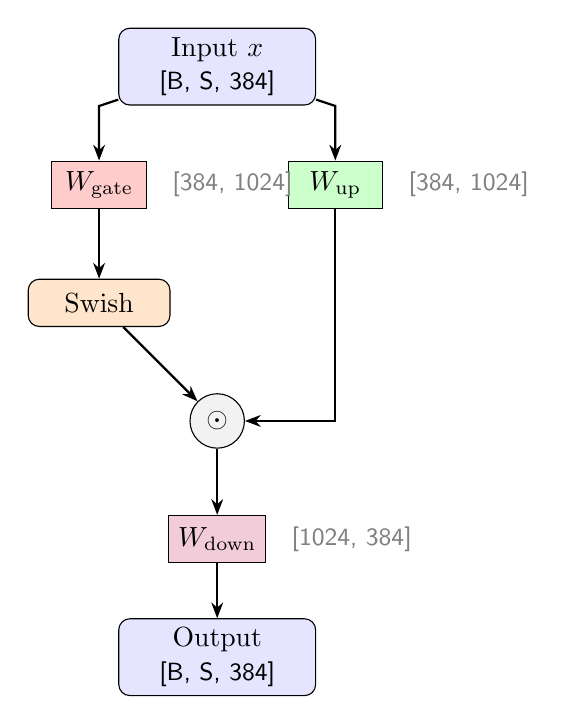
\begin{tikzpicture}[
    box/.style={rectangle, draw, rounded corners, minimum width=1.8cm, minimum height=0.6cm, fill=blue!10, align=center},
    proj/.style={rectangle, draw, minimum width=1.2cm, minimum height=0.6cm},
    op/.style={circle, draw, minimum size=0.5cm, fill=gray!10},
    arrow/.style={-{Stealth[length=2mm]}, thick},
]
    % Input
    \node[box, minimum width=2.5cm] (input) at (0, 0) {Input $x$\\\shape{B, S, 384}};

    % Gate and Up projections
    \node[proj, fill=red!20] (gate) at (-1.5, -1.5) {$W_{\text{gate}}$};
    \node[proj, fill=green!20] (up) at (1.5, -1.5) {$W_{\text{up}}$};

    % Swish activation
    \node[box, fill=orange!20] (swish) at (-1.5, -3) {Swish};

    % Element-wise multiply
    \node[op] (mul) at (0, -4.5) {$\odot$};

    % Down projection
    \node[proj, fill=purple!20] (down) at (0, -6) {$W_{\text{down}}$};

    % Output
    \node[box, minimum width=2.5cm] (output) at (0, -7.5) {Output\\\shape{B, S, 384}};

    % Arrows
    \draw[arrow] (input) -- (-1.5, -0.5) -- (gate);
    \draw[arrow] (input) -- (1.5, -0.5) -- (up);
    \draw[arrow] (gate) -- (swish);
    \draw[arrow] (swish) -- (mul);
    \draw[arrow] (up) -- (1.5, -4.5) -- (mul);
    \draw[arrow] (mul) -- (down);
    \draw[arrow] (down) -- (output);

    % Dimension annotations
    \node[font=\footnotesize, gray, right=0.2cm of gate] {\shape{384, 1024}};
    \node[font=\footnotesize, gray, right=0.2cm of up] {\shape{384, 1024}};
    \node[font=\footnotesize, gray, right=0.2cm of down] {\shape{1024, 384}};
\end{tikzpicture}
\caption{SwiGLU feed-forward network architecture}
\label{fig:swiglu}
\end{figure}

\subsection{Why SwiGLU?}

The gating mechanism allows the network to \textbf{selectively pass information}:
\begin{itemize}
    \item The ``gate'' path learns \textit{what} to let through
    \item The ``up'' path provides \textit{what} to pass
    \item Their product gives controlled information flow
\end{itemize}

Empirically, SwiGLU outperforms GELU/ReLU on language modeling benchmarks.

\subsection{Hidden Dimension}

For SwiGLU, we use $\frac{2}{3}$ of the standard hidden dimension to maintain similar parameter count:

\begin{lstlisting}[style=python, caption={FFN with SwiGLU from model.py}]
class FeedForward(nn.Module):
    def __init__(self, config: ModelConfig):
        super().__init__()

        # SwiGLU uses 2/3 of the standard hidden dim
        hidden_dim = int(2 * config.d_ff / 3)

        # Round to nearest multiple of 256 for efficiency
        hidden_dim = 256 * ((hidden_dim + 255) // 256)

        self.gate_proj = nn.Linear(config.d_model, hidden_dim, bias=False)
        self.up_proj = nn.Linear(config.d_model, hidden_dim, bias=False)
        self.down_proj = nn.Linear(hidden_dim, config.d_model, bias=False)
        self.dropout = nn.Dropout(config.dropout)

    def forward(self, x: Tensor) -> Tensor:
        # SwiGLU: swish(gate) * up
        gate = F.silu(self.gate_proj(x))  # Swish = SiLU
        up = self.up_proj(x)
        hidden = gate * up
        hidden = self.dropout(hidden)
        return self.down_proj(hidden)
\end{lstlisting}

\begin{keypoint}
For \TryLM with $d_{\text{model}} = 384$ and $d_{\text{ff}} = 1536$:
\begin{align*}
\text{hidden\_dim} &= \frac{2}{3} \times 1536 = 1024
\end{align*}
After rounding to 256: hidden\_dim = 1024 (unchanged in this case).
\end{keypoint}

% -----------------------------------------------------------------------------
\section{Pre-Normalization}
% -----------------------------------------------------------------------------

\TryLM uses \textbf{pre-normalization} (Pre-LN): normalize \textit{before} the sublayer, not after.

\subsection{Post-Norm vs Pre-Norm}

\textbf{Post-normalization} (original Transformer):
\begin{equation}
x' = \text{Norm}(x + \text{Sublayer}(x))
\end{equation}

\textbf{Pre-normalization} (\TryLM):
\begin{equation}
x' = x + \text{Sublayer}(\text{Norm}(x))
\end{equation}

\begin{figure}[H]
\centering
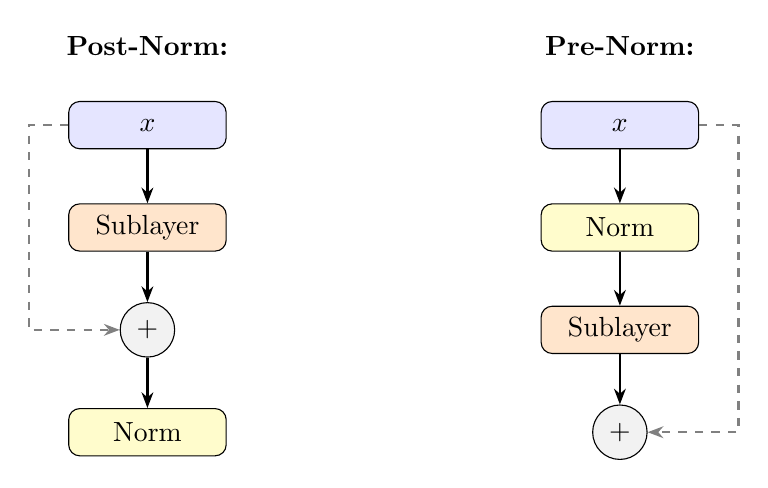
\begin{tikzpicture}[
    box/.style={rectangle, draw, rounded corners, minimum width=2cm, minimum height=0.6cm},
    arrow/.style={-{Stealth[length=2mm]}, thick},
]
    % Post-norm
    \node at (-3, 2) {\textbf{Post-Norm:}};
    \node[box, fill=blue!10] (x1) at (-3, 1) {$x$};
    \node[box, fill=orange!20] (sub1) at (-3, -0.3) {Sublayer};
    \node[circle, draw, fill=gray!10] (add1) at (-3, -1.6) {$+$};
    \node[box, fill=yellow!20] (norm1) at (-3, -2.9) {Norm};

    \draw[arrow] (x1) -- (sub1);
    \draw[arrow] (sub1) -- (add1);
    \draw[arrow] (add1) -- (norm1);
    \draw[arrow, dashed, gray] (x1.west) -- ++(-0.5, 0) |- (add1.west);

    % Pre-norm
    \node at (3, 2) {\textbf{Pre-Norm:}};
    \node[box, fill=blue!10] (x2) at (3, 1) {$x$};
    \node[box, fill=yellow!20] (norm2) at (3, -0.3) {Norm};
    \node[box, fill=orange!20] (sub2) at (3, -1.6) {Sublayer};
    \node[circle, draw, fill=gray!10] (add2) at (3, -2.9) {$+$};

    \draw[arrow] (x2) -- (norm2);
    \draw[arrow] (norm2) -- (sub2);
    \draw[arrow] (sub2) -- (add2);
    \draw[arrow, dashed, gray] (x2.east) -- ++(0.5, 0) |- (add2.east);
\end{tikzpicture}
\caption{Post-normalization (left) vs Pre-normalization (right)}
\label{fig:pre-vs-post-norm}
\end{figure}

\subsection{Why Pre-Norm?}

\begin{enumerate}
    \item \textbf{Stable gradients}: The residual connection provides a direct gradient path without normalization in the way
    \item \textbf{Easier training}: Works with larger learning rates and simpler hyperparameter tuning
    \item \textbf{No warmup required}: Post-norm often needs learning rate warmup; pre-norm is more forgiving
\end{enumerate}

\subsection{Implementation}

\begin{lstlisting}[style=python, caption={TransformerBlock with pre-norm from model.py}]
class TransformerBlock(nn.Module):
    def __init__(self, config: ModelConfig):
        super().__init__()
        self.attn_norm = RMSNorm(config.d_model)
        self.ffn_norm = RMSNorm(config.d_model)
        self.attention = MultiHeadSelfAttention(config)
        self.ffn = FeedForward(config)

    def forward(self, x: Tensor, attention_mask: Tensor | None = None) -> Tensor:
        # Pre-norm attention with residual
        x = x + self.attention(self.attn_norm(x), attention_mask)

        # Pre-norm FFN with residual
        x = x + self.ffn(self.ffn_norm(x))

        return x
\end{lstlisting}

% -----------------------------------------------------------------------------
\section{Residual Connections}
% -----------------------------------------------------------------------------

\textbf{Residual connections} (skip connections) add the input directly to the output:
\begin{equation}
\text{output} = x + f(x)
\end{equation}

\subsection{Why Residual Connections?}

\begin{enumerate}
    \item \textbf{Gradient flow}: Gradients can flow directly through the addition, avoiding vanishing gradient problems
    \item \textbf{Identity as baseline}: The layer can learn to add corrections rather than complete transformations
    \item \textbf{Deep networks}: Enable training very deep networks (GPT-3 has 96 layers!)
\end{enumerate}

\subsection{Gradient Flow Visualization}

\begin{figure}[H]
\centering
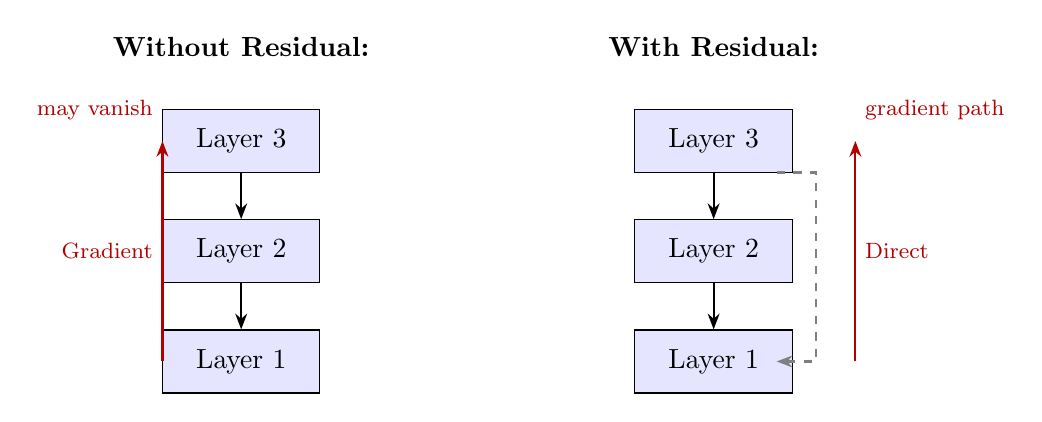
\begin{tikzpicture}[
    box/.style={rectangle, draw, minimum width=2cm, minimum height=0.8cm},
    arrow/.style={-{Stealth[length=2mm]}, thick},
    grad/.style={-{Stealth[length=2mm]}, thick, red!70!black},
]
    % Without residual
    \node at (-3, 2) {\textbf{Without Residual:}};
    \node[box, fill=blue!10] (a1) at (-3, 0.8) {Layer 3};
    \node[box, fill=blue!10] (a2) at (-3, -0.6) {Layer 2};
    \node[box, fill=blue!10] (a3) at (-3, -2) {Layer 1};

    \draw[arrow] (a1) -- (a2);
    \draw[arrow] (a2) -- (a3);

    % Gradient
    \draw[grad] (-4, -2) -- (-4, 0.8);
    \node[font=\footnotesize, red!70!black, left] at (-4, -0.6) {Gradient};
    \node[font=\footnotesize, red!70!black, left] at (-4, 1.2) {may vanish};

    % With residual
    \node at (3, 2) {\textbf{With Residual:}};
    \node[box, fill=blue!10] (b1) at (3, 0.8) {Layer 3};
    \node[box, fill=blue!10] (b2) at (3, -0.6) {Layer 2};
    \node[box, fill=blue!10] (b3) at (3, -2) {Layer 1};

    \draw[arrow] (b1) -- (b2);
    \draw[arrow] (b2) -- (b3);

    % Skip connections
    \draw[arrow, dashed, gray] (3.8, 0.4) -- ++(0.5, 0) -- ++(0, -2.4) -- ++(-0.5, 0);

    % Gradient (direct path)
    \draw[grad, thick] (4.8, -2) -- (4.8, 0.8);
    \node[font=\footnotesize, red!70!black, right] at (4.8, -0.6) {Direct};
    \node[font=\footnotesize, red!70!black, right] at (4.8, 1.2) {gradient path};
\end{tikzpicture}
\caption{Residual connections enable direct gradient flow through deep networks}
\label{fig:residual-gradient}
\end{figure}

\begin{keypoint}
Without residual connections, gradients must pass through every layer. With residuals, gradients have a ``highway'' directly back to earlier layers, enabling much deeper networks.
\end{keypoint}

% -----------------------------------------------------------------------------
\section{Dropout in Transformer Blocks}
% -----------------------------------------------------------------------------

Dropout is applied in three places within a transformer block:

\begin{enumerate}
    \item \textbf{After attention weights}: Randomly drops attention connections
    \item \textbf{After FFN hidden layer}: Regularizes the feed-forward network
    \item \textbf{After attention output projection}: Before residual addition
\end{enumerate}

\begin{lstlisting}[style=python]
# In attention:
attn_weights = self.attn_dropout(attn_weights)  # After softmax

# In FFN:
hidden = self.dropout(hidden)  # After SwiGLU, before down_proj
\end{lstlisting}

\TryLM uses \texttt{dropout=0.1} by default.

% -----------------------------------------------------------------------------
\section{The Complete Transformer Block}
% -----------------------------------------------------------------------------

Let's trace data through a complete block:

\begin{lstlisting}[style=python]
# Input: [batch=2, seq_len=128, d_model=384]
x = ...

# TransformerBlock forward pass:

# 1. Pre-norm for attention
normed = self.attn_norm(x)  # [2, 128, 384]

# 2. Multi-head self-attention
attn_out = self.attention(normed, attention_mask)  # [2, 128, 384]

# 3. Residual connection
x = x + attn_out  # [2, 128, 384]

# 4. Pre-norm for FFN
normed = self.ffn_norm(x)  # [2, 128, 384]

# 5. Feed-forward with SwiGLU
ffn_out = self.ffn(normed)  # [2, 128, 384]

# 6. Residual connection
x = x + ffn_out  # [2, 128, 384]

# Output: [2, 128, 384] (same shape as input!)
\end{lstlisting}

\begin{keypoint}
Each transformer block preserves the input shape: \texttt{[batch, seq\_len, d\_model]}. This enables stacking arbitrary numbers of blocks.
\end{keypoint}

% -----------------------------------------------------------------------------
\section{Stacking Blocks}
% -----------------------------------------------------------------------------

A complete transformer stacks multiple blocks:

\begin{lstlisting}[style=python, caption={Stacking transformer blocks from model.py}]
class GPT(nn.Module):
    def __init__(self, config: ModelConfig) -> None:
        super().__init__()
        # ...

        # Stack of transformer blocks
        self.blocks = nn.ModuleList([
            TransformerBlock(config)
            for _ in range(config.n_layers)  # 6 blocks
        ])

    def forward(self, x: Tensor, ...) -> Tensor:
        x = self.token_embedding(input_ids)
        x = self.dropout(x)

        # Pass through all blocks
        for block in self.blocks:
            x = block(x, attention_mask)

        x = self.final_norm(x)
        # ...
\end{lstlisting}

For \TryLM with 6 layers:
\begin{itemize}
    \item Each block has $\sim$1.7M parameters
    \item 6 blocks $\times$ 1.7M = $\sim$10.2M parameters
    \item Plus embeddings ($\sim$6.3M) = $\sim$10.8M total
\end{itemize}

% -----------------------------------------------------------------------------
\section{Exercises}
% -----------------------------------------------------------------------------

\begin{exercise}
\textbf{Calculate RMSNorm}

Given vector $x = [2, 4, 6]$:
\begin{enumerate}
    \item Compute the mean square: $\frac{1}{3}(2^2 + 4^2 + 6^2)$
    \item Compute the RMS: $\sqrt{\text{mean square}}$
    \item Normalize: $x / \text{RMS}$
\end{enumerate}
\end{exercise}

\begin{exercise}
\textbf{Compare Activations}

Implement and compare different activations:
\begin{lstlisting}[style=python, numbers=none]
import torch
import torch.nn.functional as F
import matplotlib.pyplot as plt

x = torch.linspace(-3, 3, 100)

plt.plot(x, F.relu(x), label='ReLU')
plt.plot(x, F.gelu(x), label='GELU')
plt.plot(x, F.silu(x), label='Swish/SiLU')
plt.legend()
\end{lstlisting}

How do they differ around $x = 0$?
\end{exercise}

\begin{exercise}
\textbf{Count Block Parameters}

For a single transformer block with $d_{\text{model}} = 384$, $d_{\text{ff}} = 1536$, and 6 attention heads, count:
\begin{enumerate}
    \item Parameters in QKV projection
    \item Parameters in output projection
    \item Parameters in FFN (gate, up, down)
    \item Parameters in both RMSNorm layers
    \item Total parameters per block
\end{enumerate}
\end{exercise}

% -----------------------------------------------------------------------------
\section{Summary}
% -----------------------------------------------------------------------------

\begin{summary}
    \item A \textbf{transformer block} = attention + FFN + residuals + norms
    \item \textbf{RMSNorm} is simpler and faster than LayerNorm, with comparable performance
    \item \textbf{SwiGLU} uses gating: $\text{Swish}(\text{gate}) \odot \text{up}$, better than GELU
    \item \textbf{Pre-normalization} normalizes before sublayers, enabling stable training
    \item \textbf{Residual connections} enable gradient flow and very deep networks
    \item Blocks preserve shape: $[B, S, D] \to [B, S, D]$, allowing arbitrary stacking
\end{summary}

Now we have all the components of a transformer block. In the next chapter, we'll assemble the complete GPT model by combining embeddings, stacked blocks, and the output projection.

% =============================================================================
% Chapter 8: The Complete GPT Model
% =============================================================================
\chapter{The Complete GPT Model}
\label{ch:complete-gpt}

\begin{objectives}
    \item Understand the complete GPT architecture
    \item Trace data flow from input to output
    \item Learn how loss is computed for language modeling
    \item Master weight initialization strategies
    \item Calculate exact parameter counts
\end{objectives}

% -----------------------------------------------------------------------------
\section{GPT Architecture Overview}
% -----------------------------------------------------------------------------

We've now covered all the components. Let's assemble them into the complete GPT model.

\begin{figure}[H]
\centering
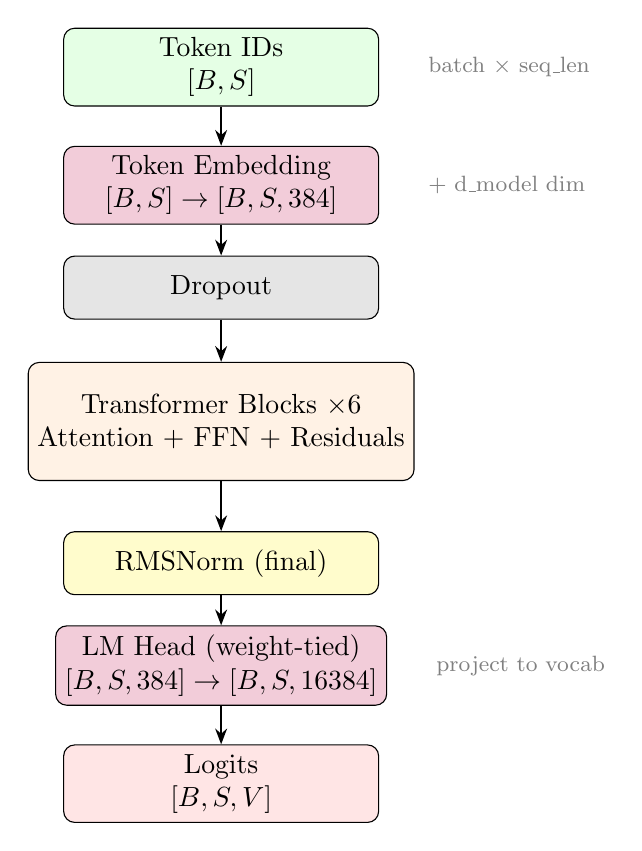
\begin{tikzpicture}[
    box/.style={rectangle, draw, rounded corners, minimum width=4cm, minimum height=0.8cm, align=center, fill=blue!10},
    block/.style={rectangle, draw, rounded corners, minimum width=4cm, minimum height=1.5cm, align=center, fill=orange!10},
    arrow/.style={-{Stealth[length=2mm]}, thick},
]
    % Input
    \node[box, fill=green!10] (input) at (0, 0) {Token IDs\\$[B, S]$};

    % Embedding
    \node[box, fill=purple!20] (emb) at (0, -1.5) {Token Embedding\\$[B, S] \to [B, S, 384]$};

    % Dropout
    \node[box, fill=gray!20] (drop) at (0, -2.8) {Dropout};

    % Transformer blocks
    \node[block] (blocks) at (0, -4.5) {Transformer Blocks $\times 6$\\Attention + FFN + Residuals};

    % Final norm
    \node[box, fill=yellow!20] (norm) at (0, -6.3) {RMSNorm (final)};

    % LM Head
    \node[box, fill=purple!20] (head) at (0, -7.6) {LM Head (weight-tied)\\$[B, S, 384] \to [B, S, 16384]$};

    % Output
    \node[box, fill=red!10] (output) at (0, -9.1) {Logits\\$[B, S, V]$};

    % Arrows
    \draw[arrow] (input) -- (emb);
    \draw[arrow] (emb) -- (drop);
    \draw[arrow] (drop) -- (blocks);
    \draw[arrow] (blocks) -- (norm);
    \draw[arrow] (norm) -- (head);
    \draw[arrow] (head) -- (output);

    % Dimension annotations
    \node[right=0.5cm of input, font=\footnotesize, gray] {batch $\times$ seq\_len};
    \node[right=0.5cm of emb, font=\footnotesize, gray] {+ d\_model dim};
    \node[right=0.5cm of head, font=\footnotesize, gray] {project to vocab};
\end{tikzpicture}
\caption{Complete GPT architecture: from token IDs to logits}
\label{fig:gpt-architecture}
\end{figure}

% -----------------------------------------------------------------------------
\section{The GPT Class}
% -----------------------------------------------------------------------------

Here's the complete model implementation:

\begin{lstlisting}[style=python, caption={GPT model from model.py}]
class GPT(nn.Module):
    def __init__(self, config: ModelConfig) -> None:
        super().__init__()
        self.config = config

        # Token embeddings
        self.token_embedding = nn.Embedding(
            config.vocab_size,    # 16384
            config.d_model,       # 384
        )

        # Dropout
        self.dropout = nn.Dropout(config.dropout)

        # Stack of transformer blocks
        self.blocks = nn.ModuleList([
            TransformerBlock(config)
            for _ in range(config.n_layers)  # 6
        ])

        # Final layer norm
        self.final_norm = RMSNorm(config.d_model)

        # Output projection (language model head)
        self.lm_head = nn.Linear(
            config.d_model,       # 384
            config.vocab_size,    # 16384
            bias=False,
        )

        # Weight tying
        self.lm_head.weight = self.token_embedding.weight

        # Initialize weights
        self.apply(self._init_weights)
\end{lstlisting}

% -----------------------------------------------------------------------------
\section{The Forward Pass}
% -----------------------------------------------------------------------------

Let's trace exactly what happens when data flows through the model.

\subsection{Input Processing}

\begin{lstlisting}[style=python, caption={Forward pass from model.py}]
def forward(
    self,
    input_ids: Tensor,              # [batch, seq_len]
    attention_mask: Tensor | None = None,
    labels: Tensor | None = None,
) -> dict[str, Tensor]:

    batch_size, seq_len = input_ids.shape

    # Step 1: Token embedding
    x = self.token_embedding(input_ids)  # [B, S, 384]
    x = self.dropout(x)
\end{lstlisting}

\subsection{Transformer Blocks}

\begin{lstlisting}[style=python]
    # Step 2: Pass through all transformer blocks
    for block in self.blocks:
        x = block(x, attention_mask)
    # Still [B, S, 384]
\end{lstlisting}

\subsection{Output Projection}

\begin{lstlisting}[style=python]
    # Step 3: Final normalization
    x = self.final_norm(x)  # [B, S, 384]

    # Step 4: Project to vocabulary
    logits = self.lm_head(x)  # [B, S, 16384]
\end{lstlisting}

\subsection{Loss Computation}

\begin{lstlisting}[style=python]
    # Step 5: Compute loss if labels provided
    if labels is not None:
        # Shift logits and labels for next-token prediction
        shift_logits = logits[..., :-1, :].contiguous()
        shift_labels = labels[..., 1:].contiguous()

        # Cross-entropy loss
        loss = F.cross_entropy(
            shift_logits.view(-1, self.config.vocab_size),
            shift_labels.view(-1),
            ignore_index=-100,  # Ignore padding
        )
        return {"logits": logits, "loss": loss}

    return {"logits": logits}
\end{lstlisting}

% -----------------------------------------------------------------------------
\section{Understanding the Loss Computation}
% -----------------------------------------------------------------------------

The loss computation involves a shift that aligns predictions with targets.

\subsection{The Shift Operation}

\begin{figure}[H]
\centering
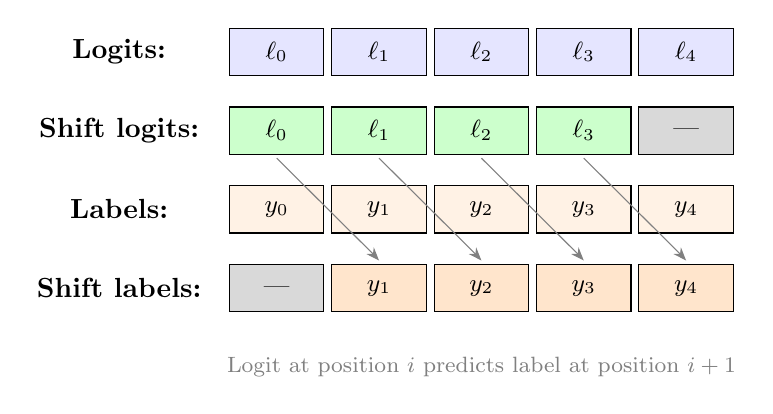
\begin{tikzpicture}[
    box/.style={rectangle, draw, minimum width=1.2cm, minimum height=0.6cm, font=\small},
]
    % Logits
    \node at (-2, 1) {\textbf{Logits:}};
    \foreach \x/\t in {0/0, 1.3/1, 2.6/2, 3.9/3, 5.2/4} {
        \node[box, fill=blue!10] at (\x, 1) {$\ell_{\t}$};
    }

    % Shifted logits (for loss)
    \node at (-2, 0) {\textbf{Shift logits:}};
    \foreach \x/\t in {0/0, 1.3/1, 2.6/2, 3.9/3} {
        \node[box, fill=green!20] at (\x, 0) {$\ell_{\t}$};
    }
    \node[box, fill=gray!30] at (5.2, 0) {---};

    % Labels
    \node at (-2, -1) {\textbf{Labels:}};
    \foreach \x/\t in {0/0, 1.3/1, 2.6/2, 3.9/3, 5.2/4} {
        \node[box, fill=orange!10] at (\x, -1) {$y_{\t}$};
    }

    % Shifted labels (for loss)
    \node at (-2, -2) {\textbf{Shift labels:}};
    \node[box, fill=gray!30] at (0, -2) {---};
    \foreach \x/\t in {1.3/1, 2.6/2, 3.9/3, 5.2/4} {
        \node[box, fill=orange!20] at (\x, -2) {$y_{\t}$};
    }

    % Alignment arrows
    \foreach \x in {0, 1.3, 2.6, 3.9} {
        \draw[-{Stealth}, gray] (\x, -0.35) -- (\x + 1.3, -1.65);
    }

    % Annotation
    \node[font=\footnotesize, gray] at (2.6, -3) {Logit at position $i$ predicts label at position $i+1$};
\end{tikzpicture}
\caption{Shift alignment: each logit predicts the next token}
\label{fig:loss-shift}
\end{figure}

\subsection{Why Shift?}

Remember the language modeling objective: predict the \textit{next} token. So:
\begin{itemize}
    \item Logits at position 0 should predict token at position 1
    \item Logits at position $n-2$ should predict token at position $n-1$
    \item Logits at position $n-1$ have nothing to predict (discarded)
\end{itemize}

\subsection{Cross-Entropy Loss}

The cross-entropy loss measures how well predictions match targets:

\begin{equation}
\mathcal{L} = -\frac{1}{N} \sum_{i=1}^{N} \log p(y_i | x_{<i})
\end{equation}

where $p(y_i | x_{<i})$ is the predicted probability of the correct next token.

\begin{keypoint}
\textbf{Perplexity} is $\exp(\mathcal{L})$---the exponential of the average loss. Lower perplexity means better predictions. A perplexity of 10 means the model is, on average, as ``surprised'' as if choosing from 10 equally likely options.
\end{keypoint}

% -----------------------------------------------------------------------------
\section{Weight Initialization}
% -----------------------------------------------------------------------------

Proper initialization is crucial for stable training.

\subsection{TryLM's Initialization Strategy}

\begin{lstlisting}[style=python, caption={Weight initialization from model.py}]
def _init_weights(self, module: nn.Module) -> None:
    if isinstance(module, nn.Linear):
        torch.nn.init.normal_(module.weight, mean=0.0, std=0.02)
        if module.bias is not None:
            torch.nn.init.zeros_(module.bias)

    elif isinstance(module, nn.Embedding):
        torch.nn.init.normal_(module.weight, mean=0.0, std=0.02)
\end{lstlisting}

\subsection{Scaled Initialization for Residuals}

Output projections get special treatment:

\begin{lstlisting}[style=python]
# Scale down residual projections
for name, p in self.named_parameters():
    if name.endswith("out_proj.weight") or name.endswith("down_proj.weight"):
        torch.nn.init.normal_(
            p,
            mean=0.0,
            std=0.02 / math.sqrt(2 * config.n_layers)
        )
\end{lstlisting}

\subsection{Why Scale?}

Residual connections sum contributions from many layers. Without scaling, the variance grows with depth:

\begin{equation}
\text{Variance after } L \text{ layers} \propto L
\end{equation}

Scaling by $1/\sqrt{2L}$ keeps variance bounded, enabling stable training of deep networks.

% -----------------------------------------------------------------------------
\section{Parameter Count}
% -----------------------------------------------------------------------------

Let's calculate the exact parameter count for \TryLM.

\subsection{Component Breakdown}

\begin{table}[H]
\centering
\begin{tabular}{lrr}
\toprule
\textbf{Component} & \textbf{Formula} & \textbf{Parameters} \\
\midrule
Token Embedding & $V \times d$ & $16384 \times 384 = 6,291,456$ \\
\addlinespace
\textit{Per Transformer Block:} & & \\
\quad QKV Projection & $d \times 3d$ & $384 \times 1152 = 442,368$ \\
\quad Output Projection & $d \times d$ & $384 \times 384 = 147,456$ \\
\quad Gate Projection & $d \times h$ & $384 \times 1024 = 393,216$ \\
\quad Up Projection & $d \times h$ & $384 \times 1024 = 393,216$ \\
\quad Down Projection & $h \times d$ & $1024 \times 384 = 393,216$ \\
\quad 2 × RMSNorm & $2 \times d$ & $2 \times 384 = 768$ \\
\quad \textit{Block Total} & & $1,770,240$ \\
\addlinespace
6 Blocks & $6 \times 1,770,240$ & $10,621,440$ \\
Final RMSNorm & $d$ & $384$ \\
LM Head & (tied with embedding) & $0$ \\
\midrule
\textbf{Total} & & $\mathbf{16,913,280}$ \\
\bottomrule
\end{tabular}
\caption{Detailed parameter breakdown for TryLM}
\label{tab:parameter-count}
\end{table}

\begin{note}
The actual count may vary slightly due to rounding in the FFN hidden dimension. The model is approximately 10.8M parameters after weight tying (since embeddings are counted once).
\end{note}

\subsection{Parameter Count Method}

\begin{lstlisting}[style=python, caption={Parameter counting from config.py}]
def count_parameters(self) -> dict[str, int]:
    """Estimate parameter counts for each component."""
    d = self.d_model
    h = int(2 * self.d_ff / 3)
    h = 256 * ((h + 255) // 256)  # Round to 256

    token_emb = self.vocab_size * d
    block_params = (
        3 * d * d +      # QKV projection
        d * d +          # Output projection
        3 * d * h +      # FFN: gate, up, down
        2 * d            # 2 RMSNorm layers
    )
    total_blocks = block_params * self.n_layers
    final_norm = d

    return {
        "token_embedding": token_emb,
        "per_block": block_params,
        "all_blocks": total_blocks,
        "final_norm": final_norm,
        "lm_head": 0,  # Tied with embedding
        "total": token_emb + total_blocks + final_norm,
    }
\end{lstlisting}

% -----------------------------------------------------------------------------
\section{Model Configuration}
% -----------------------------------------------------------------------------

The model is fully configured through the \texttt{ModelConfig} dataclass:

\begin{lstlisting}[style=python, caption={ModelConfig from config.py}]
@dataclass
class ModelConfig:
    vocab_size: int = 16384      # Vocabulary size
    n_layers: int = 6            # Number of transformer blocks
    n_heads: int = 6             # Number of attention heads
    d_model: int = 384           # Model/embedding dimension
    d_ff: int = 1536             # FFN hidden dimension
    context_length: int = 512    # Maximum sequence length
    dropout: float = 0.1         # Dropout rate
    bias: bool = False           # Use bias in linear layers

    @property
    def head_dim(self) -> int:
        return self.d_model // self.n_heads  # 384 / 6 = 64
\end{lstlisting}

% -----------------------------------------------------------------------------
\section{Model Variants}
% -----------------------------------------------------------------------------

You can easily create different model sizes by adjusting the configuration:

\begin{table}[H]
\centering
\begin{tabular}{lrrrrr}
\toprule
\textbf{Variant} & \textbf{Layers} & \textbf{Heads} & \textbf{$d$} & \textbf{FFN} & \textbf{Params} \\
\midrule
Tiny & 4 & 4 & 256 & 1024 & $\sim$5M \\
Small (default) & 6 & 6 & 384 & 1536 & $\sim$11M \\
Medium & 8 & 8 & 512 & 2048 & $\sim$25M \\
Large & 12 & 12 & 768 & 3072 & $\sim$85M \\
\bottomrule
\end{tabular}
\caption{Different model sizes by configuration}
\label{tab:model-variants}
\end{table}

\begin{lstlisting}[style=python]
# Create a medium model
config = ModelConfig(
    n_layers=8,
    n_heads=8,
    d_model=512,
    d_ff=2048,
)
model = GPT(config)
\end{lstlisting}

% -----------------------------------------------------------------------------
\section{Putting It All Together}
% -----------------------------------------------------------------------------

Here's a complete example of creating and using the model:

\begin{lstlisting}[style=python]
from trylm.model import GPT
from trylm.config import ModelConfig
from trylm.tokenizer import TryLMTokenizer
import torch

# Load tokenizer
tokenizer = TryLMTokenizer.load("data/tokenizer")

# Create model
config = ModelConfig(vocab_size=tokenizer.vocab_size)
model = GPT(config)
model.eval()

# Prepare input
text = "Once upon a time"
input_ids = torch.tensor([tokenizer.encode(text)])  # [1, seq_len]

# Forward pass (inference)
with torch.no_grad():
    outputs = model(input_ids)
    logits = outputs["logits"]  # [1, seq_len, vocab_size]

# Get prediction for next token
next_token_logits = logits[0, -1, :]  # [vocab_size]
next_token_id = next_token_logits.argmax().item()
next_token = tokenizer.decode([next_token_id])
print(f"Predicted next token: {next_token}")
\end{lstlisting}

% -----------------------------------------------------------------------------
\section{Exercises}
% -----------------------------------------------------------------------------

\begin{exercise}
\textbf{Trace Tensor Shapes}

For batch\_size=4 and seq\_len=128, trace the shape through each step:
\begin{enumerate}
    \item After token embedding
    \item After each transformer block
    \item After final norm
    \item After lm\_head
\end{enumerate}
\end{exercise}

\begin{exercise}
\textbf{Verify Weight Tying}

Check that weight tying works correctly:
\begin{lstlisting}[style=python, numbers=none]
model = GPT(ModelConfig())

# These should be the same tensor
print(model.token_embedding.weight.data_ptr())
print(model.lm_head.weight.data_ptr())

# Modify one, check the other changes
model.token_embedding.weight[0, 0] = 999.0
print(model.lm_head.weight[0, 0])  # Should be 999.0
\end{lstlisting}
\end{exercise}

\begin{exercise}
\textbf{Calculate Memory Usage}

For a batch\_size=32 and seq\_len=512 forward pass:
\begin{enumerate}
    \item Memory for model parameters (float32)
    \item Memory for attention scores (all 6 heads, all layers)
    \item Memory for activations (estimate)
\end{enumerate}
\end{exercise}

\begin{exercise}
\textbf{Create a Custom Model}

Define a custom model configuration with:
\begin{itemize}
    \item 4 layers
    \item 4 heads
    \item 256 model dimension
    \item Context length of 256
\end{itemize}

Calculate its parameter count and verify with \texttt{model.count\_parameters()}.
\end{exercise}

% -----------------------------------------------------------------------------
\section{Summary}
% -----------------------------------------------------------------------------

\begin{summary}
    \item The \textbf{GPT model} = embedding + transformer blocks + norm + output projection
    \item \textbf{Forward pass}: tokens $\to$ embeddings $\to$ blocks $\to$ norm $\to$ logits
    \item \textbf{Loss computation} uses a shift to align predictions with next-token targets
    \item \textbf{Weight initialization} uses $\mathcal{N}(0, 0.02)$ with scaled residual projections
    \item \textbf{Weight tying} shares parameters between embedding and output projection
    \item \TryLM has $\sim$\textbf{10.8M parameters} (after tying)
    \item Model size is easily \textbf{configurable} through \texttt{ModelConfig}
\end{summary}

We now have a complete understanding of the GPT architecture! In Part III, we'll learn how to train this model to actually generate coherent text.


% ============================================================================
% PART III: TRAINING
% ============================================================================
\part{Training}

% =============================================================================
% Chapter 9: The Training Loop
% =============================================================================
\chapter{The Training Loop}
\label{ch:training-loop}

\begin{objectives}
    \item Understand the complete training loop structure
    \item Learn about AdamW optimizer and weight decay
    \item Master gradient accumulation for larger effective batches
    \item Understand mixed precision training
    \item Implement gradient clipping for stability
    \item Learn about learning rate schedules
\end{objectives}

% -----------------------------------------------------------------------------
\section{Training Loop Overview}
% -----------------------------------------------------------------------------

Training a neural network is an iterative optimization process:

\begin{enumerate}
    \item \textbf{Forward pass}: Compute predictions and loss
    \item \textbf{Backward pass}: Compute gradients via backpropagation
    \item \textbf{Optimizer step}: Update weights to reduce loss
    \item \textbf{Repeat}: Until convergence or max steps
\end{enumerate}

\begin{figure}[H]
\centering
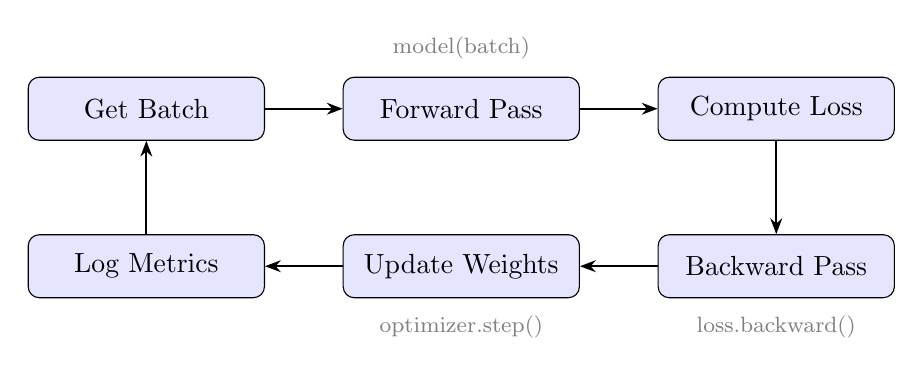
\begin{tikzpicture}[
    box/.style={rectangle, draw, rounded corners, minimum width=3cm, minimum height=0.8cm, fill=blue!10},
    arrow/.style={-{Stealth[length=2mm]}, thick},
]
    % Boxes
    \node[box] (data) at (0, 0) {Get Batch};
    \node[box] (forward) at (4, 0) {Forward Pass};
    \node[box] (loss) at (8, 0) {Compute Loss};
    \node[box] (backward) at (8, -2) {Backward Pass};
    \node[box] (update) at (4, -2) {Update Weights};
    \node[box] (log) at (0, -2) {Log Metrics};

    % Arrows
    \draw[arrow] (data) -- (forward);
    \draw[arrow] (forward) -- (loss);
    \draw[arrow] (loss) -- (backward);
    \draw[arrow] (backward) -- (update);
    \draw[arrow] (update) -- (log);
    \draw[arrow] (log) -- (data);

    % Labels
    \node[font=\footnotesize, gray, above=0.1cm of forward] {model(batch)};
    \node[font=\footnotesize, gray, below=0.1cm of backward] {loss.backward()};
    \node[font=\footnotesize, gray, below=0.1cm of update] {optimizer.step()};
\end{tikzpicture}
\caption{The training loop cycle}
\label{fig:training-loop}
\end{figure}

% -----------------------------------------------------------------------------
\section{The AdamW Optimizer}
% -----------------------------------------------------------------------------

\TryLM uses \textbf{AdamW}, the standard optimizer for transformer training.

\subsection{Adam: Adaptive Moments}

Adam maintains two moving averages for each parameter:
\begin{itemize}
    \item \textbf{First moment} ($m$): Exponential moving average of gradients
    \item \textbf{Second moment} ($v$): Exponential moving average of squared gradients
\end{itemize}

\begin{align}
m_t &= \beta_1 m_{t-1} + (1 - \beta_1) g_t \\
v_t &= \beta_2 v_{t-1} + (1 - \beta_2) g_t^2 \\
\theta_t &= \theta_{t-1} - \alpha \cdot \frac{\hat{m}_t}{\sqrt{\hat{v}_t} + \epsilon}
\end{align}

\subsection{AdamW: Decoupled Weight Decay}

AdamW separates weight decay from the gradient-based update:

\begin{equation}
\theta_t = \theta_{t-1} - \alpha \cdot \left( \frac{\hat{m}_t}{\sqrt{\hat{v}_t} + \epsilon} + \lambda \theta_{t-1} \right)
\end{equation}

\begin{keypoint}
\textbf{Weight decay} ($\lambda$) shrinks weights toward zero, acting as regularization. AdamW applies it separately from the adaptive learning rate, which empirically works better than L2 regularization.
\end{keypoint}

\subsection{Differential Weight Decay}

Not all parameters should have weight decay. We apply it only to weight matrices, not biases or normalization parameters:

\begin{lstlisting}[style=python, caption={Optimizer configuration from trainer.py}]
def _configure_optimizer(self) -> torch.optim.Optimizer:
    # Separate parameters into decay and no-decay groups
    decay_params = []
    no_decay_params = []

    for name, param in self.model.named_parameters():
        if not param.requires_grad:
            continue

        # Don't decay biases, embeddings, or normalization weights
        if param.ndim < 2 or "embedding" in name:
            no_decay_params.append(param)
        else:
            decay_params.append(param)

    optimizer = torch.optim.AdamW([
        {"params": decay_params, "weight_decay": self.config.weight_decay},
        {"params": no_decay_params, "weight_decay": 0.0},
    ],
        lr=self.config.learning_rate,  # 3e-4
        betas=(0.9, 0.95),
        eps=1e-8,
    )
    return optimizer
\end{lstlisting}

\subsection{Why Different Betas?}

\TryLM uses $\beta_1 = 0.9$ and $\beta_2 = 0.95$ (instead of the default 0.999):
\begin{itemize}
    \item Lower $\beta_2$ makes the optimizer more responsive to recent gradients
    \item This helps with the non-stationary optimization landscape of transformers
\end{itemize}

% -----------------------------------------------------------------------------
\section{Gradient Accumulation}
% -----------------------------------------------------------------------------

GPU memory limits batch size. \textbf{Gradient accumulation} simulates larger batches.

\subsection{The Problem}

Larger batches generally lead to more stable training:
\begin{itemize}
    \item Gradient estimates are less noisy
    \item Enables larger learning rates
\end{itemize}

But GPU memory limits how many sequences we can process at once.

\subsection{The Solution}

Instead of one large batch, process multiple small batches and accumulate gradients:

\begin{lstlisting}[style=python]
# Effective batch = batch_size * gradient_accumulation_steps
# 256 = 64 * 4

for step in range(max_steps):
    optimizer.zero_grad()

    # Accumulate gradients over multiple micro-batches
    for micro_step in range(gradient_accumulation_steps):
        batch = next(data_iter)
        loss = model(batch)["loss"]

        # Scale loss by accumulation steps
        (loss / gradient_accumulation_steps).backward()

    # Update weights once per effective batch
    optimizer.step()
\end{lstlisting}

\begin{figure}[H]
\centering
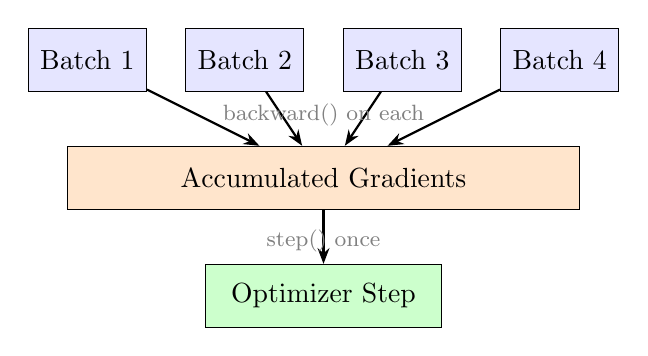
\begin{tikzpicture}[
    box/.style={rectangle, draw, minimum width=1.5cm, minimum height=0.8cm, fill=blue!10},
    acc/.style={rectangle, draw, minimum width=1.5cm, minimum height=0.8cm, fill=orange!20},
    arrow/.style={-{Stealth[length=2mm]}, thick},
]
    % Micro batches
    \node[box] (b1) at (0, 0) {Batch 1};
    \node[box] (b2) at (2, 0) {Batch 2};
    \node[box] (b3) at (4, 0) {Batch 3};
    \node[box] (b4) at (6, 0) {Batch 4};

    % Gradient accumulation
    \node[acc, minimum width=6.5cm] (acc) at (3, -1.5) {Accumulated Gradients};

    % Optimizer step
    \node[box, fill=green!20, minimum width=3cm] (step) at (3, -3) {Optimizer Step};

    % Arrows
    \foreach \b in {b1, b2, b3, b4} {
        \draw[arrow] (\b) -- (acc);
    }
    \draw[arrow] (acc) -- (step);

    % Labels
    \node[font=\footnotesize, gray] at (3, -0.7) {backward() on each};
    \node[font=\footnotesize, gray] at (3, -2.3) {step() once};
\end{tikzpicture}
\caption{Gradient accumulation: 4 batches contribute to one optimizer step}
\label{fig:gradient-accumulation}
\end{figure}

\begin{keypoint}
With batch\_size=64 and gradient\_accumulation\_steps=4, the \textbf{effective batch size} is $64 \times 4 = 256$ sequences.
\end{keypoint}

% -----------------------------------------------------------------------------
\section{Mixed Precision Training}
% -----------------------------------------------------------------------------

\textbf{Mixed precision} uses lower-precision (float16/bfloat16) for most computations while maintaining float32 for critical operations.

\subsection{Benefits}

\begin{enumerate}
    \item \textbf{Faster}: GPUs compute float16 much faster
    \item \textbf{Less memory}: Half the bytes per number
    \item \textbf{Larger batches}: More sequences fit in memory
\end{enumerate}

\subsection{Challenges}

Float16 has limited range ($\sim 10^{-5}$ to $\sim 65504$):
\begin{itemize}
    \item Gradients can underflow (become zero)
    \item Weights updates may be too small to represent
\end{itemize}

\subsection{Loss Scaling}

\textbf{GradScaler} automatically scales the loss to prevent underflow:

\begin{lstlisting}[style=python, caption={Mixed precision training from trainer.py}]
from torch.cuda.amp import autocast, GradScaler

# Create scaler
scaler = GradScaler() if mixed_precision else None

for batch in dataloader:
    optimizer.zero_grad()

    # Forward pass in mixed precision
    with autocast(enabled=mixed_precision):
        outputs = model(**batch)
        loss = outputs["loss"] / gradient_accumulation_steps

    # Backward with scaled loss
    if scaler is not None:
        scaler.scale(loss).backward()
    else:
        loss.backward()

    # Optimizer step with unscaling
    if scaler is not None:
        scaler.unscale_(optimizer)
        # Gradient clipping here
        scaler.step(optimizer)
        scaler.update()
    else:
        optimizer.step()
\end{lstlisting}

\begin{keypoint}
\texttt{autocast} automatically chooses float16 vs float32 for each operation. Matmuls use float16; reductions (softmax, norms) use float32 for accuracy.
\end{keypoint}

% -----------------------------------------------------------------------------
\section{Gradient Clipping}
% -----------------------------------------------------------------------------

\textbf{Gradient clipping} prevents exploding gradients by limiting their magnitude.

\subsection{Why Clip?}

During training, gradients can occasionally become very large:
\begin{itemize}
    \item Causes weight updates that overshoot
    \item Can destabilize or crash training
    \item Particularly common early in training
\end{itemize}

\subsection{Max Norm Clipping}

We clip by scaling gradients if their total norm exceeds a threshold:

\begin{equation}
\mathbf{g}' = \begin{cases}
\mathbf{g} & \text{if } \|\mathbf{g}\| \leq \text{max\_norm} \\
\frac{\text{max\_norm}}{\|\mathbf{g}\|} \cdot \mathbf{g} & \text{otherwise}
\end{cases}
\end{equation}

\begin{lstlisting}[style=python, caption={Gradient clipping from trainer.py}]
# After backward, before optimizer step
torch.nn.utils.clip_grad_norm_(
    model.parameters(),
    max_norm=self.config.grad_clip,  # 1.0
)
\end{lstlisting}

\begin{keypoint}
\TryLM uses \texttt{grad\_clip=1.0}. This means gradient vectors are scaled down if their L2 norm exceeds 1.0, preserving direction but limiting magnitude.
\end{keypoint}

% -----------------------------------------------------------------------------
\section{Learning Rate Schedule}
% -----------------------------------------------------------------------------

A fixed learning rate is suboptimal. We use a \textbf{schedule} that varies the learning rate during training.

\subsection{Warmup + Cosine Decay}

\TryLM uses:
\begin{enumerate}
    \item \textbf{Linear warmup}: LR increases from 0 to max over warmup steps
    \item \textbf{Cosine decay}: LR decreases following a cosine curve
\end{enumerate}

\begin{figure}[H]
\centering
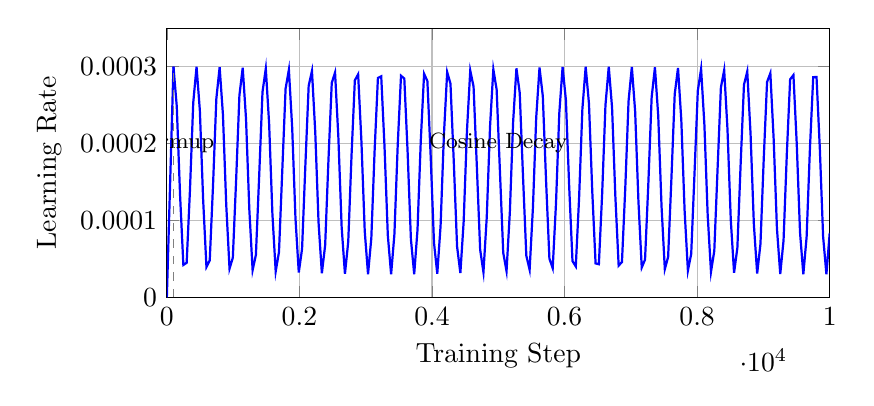
\begin{tikzpicture}
    \begin{axis}[
        width=10cm,
        height=5cm,
        xlabel={Training Step},
        ylabel={Learning Rate},
        xmin=0, xmax=10000,
        ymin=0, ymax=3.5e-4,
        grid=major,
        scaled y ticks=false,
        yticklabel style={
            /pgf/number format/fixed,
            /pgf/number format/precision=4
        },
    ]
        % Warmup phase
        \addplot[thick, blue, domain=0:100] {3e-4 * x / 100};

        % Cosine decay phase
        \addplot[thick, blue, domain=100:10000, samples=200]
            {3e-5 + (3e-4 - 3e-5) * (1 + cos(deg((x-100)/(10000-100) * 180))) / 2};

        % Annotations
        \node[font=\footnotesize] at (axis cs:50, 2e-4) {Warmup};
        \node[font=\footnotesize] at (axis cs:5000, 2e-4) {Cosine Decay};
        \draw[dashed, gray] (axis cs:100, 0) -- (axis cs:100, 3e-4);
    \end{axis}
\end{tikzpicture}
\caption{Learning rate schedule: linear warmup then cosine decay}
\label{fig:lr-schedule}
\end{figure}

\subsection{Implementation}

\begin{lstlisting}[style=python, caption={LR schedule from trainer.py}]
def get_lr(step: int, config: TrainConfig) -> float:
    """Cosine learning rate schedule with warmup."""
    # Warmup phase
    if step < config.warmup_steps:
        return config.learning_rate * (step / config.warmup_steps)

    # Cosine decay phase
    progress = (step - config.warmup_steps) / (
        config.max_steps - config.warmup_steps
    )
    min_lr = config.learning_rate * 0.1  # Decay to 10% of max

    return min_lr + (config.learning_rate - min_lr) * (
        1 + math.cos(math.pi * progress)
    ) / 2
\end{lstlisting}

\subsection{Why This Schedule?}

\begin{itemize}
    \item \textbf{Warmup}: Early training is unstable; small LR prevents divergence
    \item \textbf{High LR}: Enables fast learning in the middle
    \item \textbf{Decay}: Fine-grained optimization at the end
\end{itemize}

% -----------------------------------------------------------------------------
\section{The Complete Training Step}
% -----------------------------------------------------------------------------

Here's how all components come together:

\begin{lstlisting}[style=python, caption={Complete training step from trainer.py}]
def train(self) -> None:
    self.model.train()
    data_iter = iter(self.train_loader)

    for step in range(self.start_step, self.config.max_steps):
        # Update learning rate
        lr = get_lr(step, self.config)
        for param_group in self.optimizer.param_groups:
            param_group["lr"] = lr

        # Gradient accumulation loop
        self.optimizer.zero_grad()
        total_loss = 0.0

        for micro_step in range(self.config.gradient_accumulation_steps):
            batch = next(data_iter)
            batch = {k: v.to(self.device) for k, v in batch.items()}

            # Forward pass with mixed precision
            with autocast(enabled=self.mixed_precision):
                outputs = self.model(**batch)
                loss = outputs["loss"]
                loss = loss / self.config.gradient_accumulation_steps

            total_loss += loss.item()

            # Backward pass
            if self.scaler is not None:
                self.scaler.scale(loss).backward()
            else:
                loss.backward()

        # Gradient clipping and optimizer step
        if self.scaler is not None:
            self.scaler.unscale_(self.optimizer)

        grad_norm = torch.nn.utils.clip_grad_norm_(
            self.model.parameters(),
            self.config.grad_clip,
        )

        if self.scaler is not None:
            self.scaler.step(self.optimizer)
            self.scaler.update()
        else:
            self.optimizer.step()

        # Logging
        if step % self.config.log_interval == 0:
            self.log_metrics(step, total_loss, grad_norm, lr)
\end{lstlisting}

% -----------------------------------------------------------------------------
\section{Running Training}
% -----------------------------------------------------------------------------

\subsection{Using the CLI}

\begin{lstlisting}[style=shell]
# Train with default config
uv run trylm train

# Train with custom parameters
uv run trylm train \
    --config configs/tiny_stories.yaml \
    --batch-size 32 \
    --max-steps 5000 \
    --learning-rate 1e-4

# Resume from checkpoint
uv run trylm train --resume checkpoints/step_5000
\end{lstlisting}

\subsection{Expected Output}

\begin{lstlisting}[style=shell, numbers=none]
Training TryLM...
Device: cuda
Model parameters: 10,821,120

Step     0 | Loss: 10.234 | PPL: 27826 | LR: 0.00000 | Grad: 2.31
Step    10 | Loss:  9.456 | PPL: 12806 | LR: 0.00003 | Grad: 1.82
Step    20 | Loss:  8.123 | PPL:  3375 | LR: 0.00006 | Grad: 1.45
...
Step  1000 | Loss:  3.456 | PPL:    31 | LR: 0.00029 | Grad: 0.67
\end{lstlisting}

% -----------------------------------------------------------------------------
\section{Exercises}
% -----------------------------------------------------------------------------

\begin{exercise}
\textbf{Calculate Effective Batch Size}

With batch\_size=64, gradient\_accumulation\_steps=4, and 4 GPUs using data parallelism, what is the effective batch size?
\end{exercise}

\begin{exercise}
\textbf{Learning Rate Calculation}

For warmup\_steps=100, max\_steps=10000, and learning\_rate=3e-4:
\begin{enumerate}
    \item What is the LR at step 50?
    \item What is the LR at step 100?
    \item What is the LR at step 5000?
    \item What is the LR at step 9900?
\end{enumerate}
\end{exercise}

\begin{exercise}
\textbf{Gradient Clipping Experiment}

Train the same model with different grad\_clip values:
\begin{lstlisting}[style=shell, numbers=none]
uv run trylm train --max-steps 1000 --grad-clip 0.5
uv run trylm train --max-steps 1000 --grad-clip 1.0
uv run trylm train --max-steps 1000 --grad-clip 5.0
\end{lstlisting}

How does the training loss curve differ?
\end{exercise}

% -----------------------------------------------------------------------------
\section{Summary}
% -----------------------------------------------------------------------------

\begin{summary}
    \item The \textbf{training loop}: forward $\to$ backward $\to$ optimize $\to$ repeat
    \item \textbf{AdamW} with differential weight decay is standard for transformers
    \item \textbf{Gradient accumulation} enables larger effective batches than GPU memory allows
    \item \textbf{Mixed precision} (float16) speeds training and reduces memory
    \item \textbf{Gradient clipping} prevents exploding gradients
    \item \textbf{LR schedule}: warmup + cosine decay for stable, effective training
\end{summary}

Training is now running! In the next chapter, we'll learn how to monitor progress, save checkpoints, and ensure reproducibility.

% =============================================================================
% Chapter 10: Monitoring and Checkpointing
% =============================================================================
\chapter{Monitoring and Checkpointing}
\label{ch:monitoring-checkpointing}

\begin{objectives}
    \item Use Weights \& Biases for experiment tracking
    \item Implement robust checkpointing
    \item Resume training from checkpoints
    \item Ensure reproducibility with seeds
\end{objectives}

% -----------------------------------------------------------------------------
\section{Experiment Tracking with W\&B}
% -----------------------------------------------------------------------------

\textbf{Weights \& Biases} (W\&B) provides cloud-based experiment tracking.

\subsection{What W\&B Logs}

\TryLM logs:
\begin{itemize}
    \item \textbf{Metrics}: Loss, perplexity, gradient norm, learning rate
    \item \textbf{Config}: All hyperparameters
    \item \textbf{Samples}: Generated text examples during training
    \item \textbf{System}: GPU memory, utilization
\end{itemize}

\subsection{Enabling W\&B}

\begin{lstlisting}[style=shell]
# Login (one-time)
uv run wandb login

# Train with logging
uv run trylm train --wandb-project trylm --wandb-run my-experiment
\end{lstlisting}

\subsection{Implementation}

\begin{lstlisting}[style=python, caption={W\&B logging from trainer.py}]
import wandb

# Initialize
wandb.init(
    project=config.wandb_project,
    name=config.wandb_run_name,
    config=asdict(config),
)

# Log metrics
wandb.log({
    "train/loss": loss,
    "train/perplexity": math.exp(loss),
    "train/learning_rate": lr,
    "train/grad_norm": grad_norm,
}, step=step)

# Log generated samples
samples = generate_samples(model, tokenizer)
wandb.log({"samples": wandb.Table(data=samples)}, step=step)
\end{lstlisting}

% -----------------------------------------------------------------------------
\section{Checkpointing}
% -----------------------------------------------------------------------------

Checkpoints save training state so you can resume or use the model later.

\subsection{Checkpoint Contents}

\begin{lstlisting}[style=shell, numbers=none]
checkpoints/step_5000/
|-- model.safetensors      # Model weights
|-- training_state.pt      # Optimizer, scheduler, step
`-- config.yaml            # Full configuration
\end{lstlisting}

\subsection{Saving Checkpoints}

\begin{lstlisting}[style=python, caption={Checkpoint saving from trainer.py}]
from safetensors.torch import save_file

def save_checkpoint(self, path: Path, step: int) -> None:
    path.mkdir(parents=True, exist_ok=True)

    # Save model weights with safetensors
    state_dict = self.model.state_dict()
    save_file(state_dict, path / "model.safetensors")

    # Save training state
    torch.save({
        "step": step,
        "optimizer": self.optimizer.state_dict(),
        "scheduler": self.scheduler.state_dict() if self.scheduler else None,
        "scaler": self.scaler.state_dict() if self.scaler else None,
        "best_val_loss": self.best_val_loss,
    }, path / "training_state.pt")

    # Save config for reproducibility
    self.full_config.to_yaml(path / "config.yaml")
\end{lstlisting}

\subsection{Loading Checkpoints}

\begin{lstlisting}[style=python, caption={Checkpoint loading from trainer.py}]
from safetensors.torch import load_file

def load_checkpoint(self, path: Path) -> int:
    # Load model weights
    state_dict = load_file(path / "model.safetensors")
    self.model.load_state_dict(state_dict)

    # Load training state
    training_state = torch.load(path / "training_state.pt")
    self.optimizer.load_state_dict(training_state["optimizer"])
    if self.scheduler and training_state["scheduler"]:
        self.scheduler.load_state_dict(training_state["scheduler"])
    if self.scaler and training_state["scaler"]:
        self.scaler.load_state_dict(training_state["scaler"])

    return training_state["step"]
\end{lstlisting}

\subsection{Checkpoint Strategy}

\TryLM saves checkpoints at three points:
\begin{enumerate}
    \item \textbf{Regular intervals}: Every \texttt{save\_interval} steps (default: 1000)
    \item \textbf{Best model}: When validation loss improves
    \item \textbf{Final}: At training completion
\end{enumerate}

% -----------------------------------------------------------------------------
\section{Resuming Training}
% -----------------------------------------------------------------------------

\begin{lstlisting}[style=shell]
# Resume from a specific checkpoint
uv run trylm train --resume checkpoints/step_5000

# Resume from best checkpoint
uv run trylm train --resume checkpoints/best
\end{lstlisting}

Resuming restores:
\begin{itemize}
    \item Model weights
    \item Optimizer state (momentum, adaptive learning rates)
    \item Training step counter
    \item Learning rate scheduler state
    \item Mixed precision scaler state
\end{itemize}

% -----------------------------------------------------------------------------
\section{Reproducibility}
% -----------------------------------------------------------------------------

\subsection{Setting Seeds}

\begin{lstlisting}[style=python]
def set_seed(seed: int) -> None:
    random.seed(seed)
    np.random.seed(seed)
    torch.manual_seed(seed)
    torch.cuda.manual_seed_all(seed)
\end{lstlisting}

\subsection{Deterministic Operations}

\begin{lstlisting}[style=python]
# For full reproducibility (slower)
torch.backends.cudnn.deterministic = True
torch.backends.cudnn.benchmark = False
\end{lstlisting}

\begin{keypoint}
Even with seeds set, GPU operations may have non-deterministic behavior. For true reproducibility, save checkpoints frequently and validate on held-out data.
\end{keypoint}

% -----------------------------------------------------------------------------
\section{Summary}
% -----------------------------------------------------------------------------

\begin{summary}
    \item \textbf{W\&B} provides cloud experiment tracking with metrics, configs, and samples
    \item \textbf{Checkpoints} save model, optimizer, and scheduler state
    \item \textbf{Safetensors} format is safe and efficient for model weights
    \item \textbf{Resume training} restores complete state from checkpoint
    \item \textbf{Seeds} enable approximate reproducibility
\end{summary}

% =============================================================================
% Chapter 11: Evaluation
% =============================================================================
\chapter{Evaluation}
\label{ch:evaluation}

\begin{objectives}
    \item Understand perplexity as an evaluation metric
    \item Compute perplexity on validation data
    \item Perform qualitative evaluation through generation
    \item Detect and prevent overfitting
\end{objectives}

% -----------------------------------------------------------------------------
\section{Perplexity}
% -----------------------------------------------------------------------------

\textbf{Perplexity} is the standard metric for language models.

\subsection{Definition}

Perplexity is the exponential of the average cross-entropy loss:

\begin{equation}
\text{PPL} = \exp\left(-\frac{1}{N}\sum_{i=1}^{N} \log p(x_i | x_{<i})\right) = \exp(\mathcal{L})
\end{equation}

\subsection{Interpretation}

Perplexity can be thought of as ``effective vocabulary size'':
\begin{itemize}
    \item PPL = 10 means the model is as uncertain as choosing from 10 equally likely tokens
    \item PPL = 100 means choosing from 100 equally likely tokens
    \item \textbf{Lower is better}
\end{itemize}

\subsection{Typical Values}

\begin{table}[H]
\centering
\begin{tabular}{ll}
\toprule
\textbf{Model/Dataset} & \textbf{Perplexity} \\
\midrule
Random (vocab=16K) & 16,384 \\
Untrained TryLM & $\sim$16,000 \\
Trained TryLM (TinyStories) & 20--40 \\
GPT-2 (WebText) & $\sim$20 \\
\bottomrule
\end{tabular}
\caption{Typical perplexity values}
\end{table}

% -----------------------------------------------------------------------------
\section{Computing Perplexity}
% -----------------------------------------------------------------------------

\begin{lstlisting}[style=python, caption={Perplexity computation from evaluate.py}]
@torch.no_grad()
def compute_perplexity(
    model: GPT,
    dataloader: DataLoader,
    device: str,
    max_batches: int | None = None,
) -> float:
    model.eval()
    total_loss = 0.0
    total_tokens = 0

    for i, batch in enumerate(dataloader):
        if max_batches and i >= max_batches:
            break

        batch = {k: v.to(device) for k, v in batch.items()}
        outputs = model(**batch)
        loss = outputs["loss"]

        # Count non-padding tokens
        mask = batch["labels"] != -100
        num_tokens = mask.sum().item()

        total_loss += loss.item() * num_tokens
        total_tokens += num_tokens

    avg_loss = total_loss / total_tokens
    perplexity = math.exp(avg_loss)

    return perplexity
\end{lstlisting}

\subsection{Using the CLI}

\begin{lstlisting}[style=shell]
uv run trylm eval --checkpoint checkpoints/best

# Output:
# Validation Perplexity: 28.45
\end{lstlisting}

% -----------------------------------------------------------------------------
\section{Qualitative Evaluation}
% -----------------------------------------------------------------------------

Numbers don't tell the whole story. Generate samples to assess quality.

\subsection{Sample Prompts}

\begin{lstlisting}[style=python]
prompts = [
    "Once upon a time",
    "The little girl",
    "One day, a boy named",
]

for prompt in prompts:
    output = generate(model, tokenizer, prompt, max_new_tokens=100)
    print(f"Prompt: {prompt}")
    print(f"Output: {output}\n")
\end{lstlisting}

\subsection{What to Look For}

\begin{itemize}
    \item \textbf{Grammar}: Are sentences well-formed?
    \item \textbf{Coherence}: Does the story make sense?
    \item \textbf{Creativity}: Is it interesting or just repetitive?
    \item \textbf{Completion}: Does it reach a natural ending?
\end{itemize}

% -----------------------------------------------------------------------------
\section{Train vs. Validation}
% -----------------------------------------------------------------------------

Compare perplexity on training and validation data:

\begin{itemize}
    \item \textbf{Similar}: Model generalizes well
    \item \textbf{Train << Val}: Overfitting (memorizing training data)
    \item \textbf{Both high}: Underfitting (model too small or undertrained)
\end{itemize}

\begin{figure}[H]
\centering
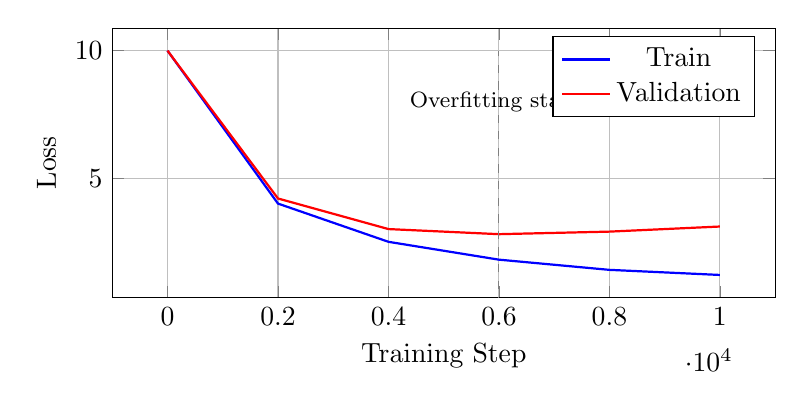
\begin{tikzpicture}
    \begin{axis}[
        width=10cm,
        height=5cm,
        xlabel={Training Step},
        ylabel={Loss},
        legend pos=north east,
        grid=major,
    ]
        \addplot[thick, blue] coordinates {
            (0, 10) (2000, 4) (4000, 2.5) (6000, 1.8) (8000, 1.4) (10000, 1.2)
        };
        \addlegendentry{Train}

        \addplot[thick, red] coordinates {
            (0, 10) (2000, 4.2) (4000, 3.0) (6000, 2.8) (8000, 2.9) (10000, 3.1)
        };
        \addlegendentry{Validation}

        \draw[dashed, gray] (axis cs:6000, 0) -- (axis cs:6000, 10);
        \node[font=\footnotesize] at (axis cs:6000, 8) {Overfitting starts};
    \end{axis}
\end{tikzpicture}
\caption{Detecting overfitting: validation loss increases while training loss decreases}
\label{fig:overfitting}
\end{figure}

% -----------------------------------------------------------------------------
\section{Summary}
% -----------------------------------------------------------------------------

\begin{summary}
    \item \textbf{Perplexity} = $\exp(\text{loss})$; lower is better
    \item Perplexity represents ``effective vocabulary size'' of uncertainty
    \item \textbf{Qualitative evaluation} through generation catches issues metrics miss
    \item Compare \textbf{train vs. validation} loss to detect overfitting
    \item Good TryLM performance: PPL 20--40 on TinyStories validation
\end{summary}


% ============================================================================
% PART IV: GENERATION AND BEYOND
% ============================================================================
\part{Generation and Beyond}

% =============================================================================
% Chapter 12: Text Generation
% =============================================================================
\chapter{Text Generation}
\label{ch:text-generation}

\begin{objectives}
    \item Understand autoregressive generation
    \item Master temperature scaling
    \item Implement top-k and top-p (nucleus) sampling
    \item Use repetition penalty
    \item Build an interactive generation interface
\end{objectives}

% -----------------------------------------------------------------------------
\section{Autoregressive Generation}
% -----------------------------------------------------------------------------

Generation works by repeatedly predicting the next token:

\begin{algorithm}[H]
\caption{Autoregressive Text Generation}
\begin{algorithmic}[1]
\Require Prompt tokens, model, max tokens
\State tokens $\gets$ encode(prompt)
\While{len(tokens) $<$ max\_length \textbf{and} tokens[-1] $\neq$ EOS}
    \State logits $\gets$ model(tokens)[-1]  \Comment{Last position logits}
    \State next\_token $\gets$ sample(logits)  \Comment{Sampling strategy}
    \State tokens.append(next\_token)
\EndWhile
\State \Return decode(tokens)
\end{algorithmic}
\end{algorithm}

\begin{lstlisting}[style=python, caption={Core generation loop from generate.py}]
@torch.no_grad()
def generate(
    model: GPT,
    tokenizer: TryLMTokenizer,
    prompt: str,
    max_new_tokens: int = 100,
    temperature: float = 1.0,
    top_k: int = 0,
    top_p: float = 1.0,
) -> str:
    model.eval()
    input_ids = torch.tensor([tokenizer.encode(prompt)])

    for _ in range(max_new_tokens):
        # Get logits for last position
        outputs = model(input_ids)
        next_token_logits = outputs["logits"][0, -1, :]

        # Apply sampling
        next_token_logits = next_token_logits / temperature
        if top_k > 0:
            next_token_logits = top_k_filtering(next_token_logits, top_k)
        if top_p < 1.0:
            next_token_logits = top_p_filtering(next_token_logits, top_p)

        # Sample
        probs = F.softmax(next_token_logits, dim=-1)
        next_token = torch.multinomial(probs, num_samples=1)

        # Append and check for EOS
        input_ids = torch.cat([input_ids, next_token.unsqueeze(0)], dim=1)
        if next_token.item() == tokenizer.eos_id:
            break

    return tokenizer.decode(input_ids[0].tolist())
\end{lstlisting}

% -----------------------------------------------------------------------------
\section{Temperature}
% -----------------------------------------------------------------------------

\textbf{Temperature} controls randomness by scaling logits before softmax:

\begin{equation}
p_i = \frac{\exp(z_i / T)}{\sum_j \exp(z_j / T)}
\end{equation}

\begin{itemize}
    \item $T < 1$: Sharper distribution (more deterministic)
    \item $T = 1$: Original distribution
    \item $T > 1$: Flatter distribution (more random)
\end{itemize}

\begin{figure}[H]
\centering
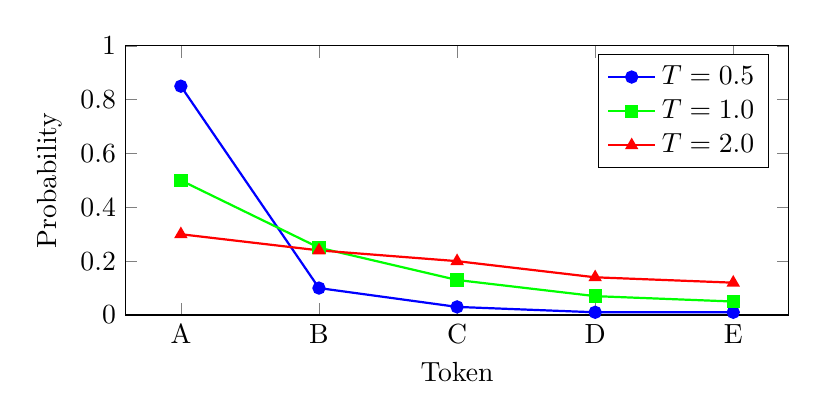
\begin{tikzpicture}
    \begin{axis}[
        width=10cm,
        height=5cm,
        xlabel={Token},
        ylabel={Probability},
        ymin=0, ymax=1,
        legend pos=north east,
        xtick={1,2,3,4,5},
        xticklabels={A, B, C, D, E},
    ]
        % T=0.5
        \addplot[thick, blue, mark=*] coordinates {
            (1, 0.85) (2, 0.10) (3, 0.03) (4, 0.01) (5, 0.01)
        };
        \addlegendentry{$T=0.5$}

        % T=1.0
        \addplot[thick, green, mark=square*] coordinates {
            (1, 0.50) (2, 0.25) (3, 0.13) (4, 0.07) (5, 0.05)
        };
        \addlegendentry{$T=1.0$}

        % T=2.0
        \addplot[thick, red, mark=triangle*] coordinates {
            (1, 0.30) (2, 0.24) (3, 0.20) (4, 0.14) (5, 0.12)
        };
        \addlegendentry{$T=2.0$}
    \end{axis}
\end{tikzpicture}
\caption{Effect of temperature on probability distribution}
\label{fig:temperature}
\end{figure}

% -----------------------------------------------------------------------------
\section{Top-k Filtering}
% -----------------------------------------------------------------------------

\textbf{Top-k sampling} keeps only the $k$ most likely tokens:

\begin{lstlisting}[style=python, caption={Top-k filtering from generate.py}]
def top_k_filtering(logits: Tensor, k: int) -> Tensor:
    if k <= 0:
        return logits

    # Find the k-th largest value
    values, _ = torch.topk(logits, k)
    min_value = values[-1]

    # Set all values below threshold to -inf
    return torch.where(
        logits < min_value,
        torch.full_like(logits, float("-inf")),
        logits,
    )
\end{lstlisting}

% -----------------------------------------------------------------------------
\section{Top-p (Nucleus) Sampling}
% -----------------------------------------------------------------------------

\textbf{Top-p sampling} keeps the smallest set of tokens whose cumulative probability exceeds $p$:

\begin{lstlisting}[style=python, caption={Top-p filtering from generate.py}]
def top_p_filtering(logits: Tensor, p: float) -> Tensor:
    sorted_logits, sorted_indices = torch.sort(logits, descending=True)
    cumulative_probs = torch.cumsum(F.softmax(sorted_logits, dim=-1), dim=-1)

    # Find cutoff index
    sorted_indices_to_remove = cumulative_probs > p
    sorted_indices_to_remove[1:] = sorted_indices_to_remove[:-1].clone()
    sorted_indices_to_remove[0] = False

    # Remove tokens beyond cutoff
    indices_to_remove = sorted_indices[sorted_indices_to_remove]
    logits[indices_to_remove] = float("-inf")

    return logits
\end{lstlisting}

\begin{keypoint}
Top-p is more adaptive than top-k:
\begin{itemize}
    \item When the model is confident, fewer tokens are kept
    \item When uncertain, more tokens are allowed
\end{itemize}
\end{keypoint}

% -----------------------------------------------------------------------------
\section{Repetition Penalty}
% -----------------------------------------------------------------------------

To avoid repetitive text, penalize tokens that have already appeared:

\begin{lstlisting}[style=python]
def apply_repetition_penalty(
    logits: Tensor,
    generated_tokens: list[int],
    penalty: float = 1.2,
) -> Tensor:
    for token_id in set(generated_tokens):
        if logits[token_id] > 0:
            logits[token_id] /= penalty
        else:
            logits[token_id] *= penalty
    return logits
\end{lstlisting}

% -----------------------------------------------------------------------------
\section{Generation Examples}
% -----------------------------------------------------------------------------

\begin{lstlisting}[style=shell]
# Basic generation
uv run trylm generate "Once upon a time"

# Adjust parameters
uv run trylm generate "The princess" \
    --temperature 0.8 \
    --top-k 50 \
    --top-p 0.9 \
    --max-tokens 200

# Interactive mode
uv run trylm generate -i
\end{lstlisting}

\subsection{Interactive Mode}

\begin{lstlisting}[style=shell, numbers=none]
TryLM Interactive Mode
Commands: :temp <v>, :top_p <v>, :max <v>, :quit

> Once upon a time there was a little rabbit.
The rabbit liked to hop in the garden. One day,
the rabbit found a big carrot...

> :temp 0.5
Temperature set to 0.5

> The king
The king was very happy. He had a beautiful castle.
\end{lstlisting}

% -----------------------------------------------------------------------------
\section{Summary}
% -----------------------------------------------------------------------------

\begin{summary}
    \item \textbf{Autoregressive generation}: predict one token at a time, append, repeat
    \item \textbf{Temperature}: controls randomness ($<1$ = focused, $>1$ = diverse)
    \item \textbf{Top-k}: keep only $k$ most likely tokens
    \item \textbf{Top-p (nucleus)}: keep tokens until cumulative probability $> p$
    \item \textbf{Repetition penalty}: discourage repeating tokens
    \item Recommended defaults: temperature=0.8, top\_p=0.9, top\_k=50
\end{summary}

% =============================================================================
% Chapter 13: End-to-End Workflow
% =============================================================================
\chapter{End-to-End Workflow}
\label{ch:end-to-end}

\begin{objectives}
    \item Execute the complete training pipeline
    \item Learn hyperparameter tuning strategies
    \item Debug common training issues
    \item Document and share your model
\end{objectives}

% -----------------------------------------------------------------------------
\section{Complete Pipeline}
% -----------------------------------------------------------------------------

Here's the full workflow from start to finish:

\begin{lstlisting}[style=shell]
# 1. Setup
git clone https://github.com/your-repo/trylm.git
cd trylm
uv sync

# 2. Train tokenizer
uv run trylm tokenizer train --vocab-size 16384

# 3. Train model
uv run trylm train \
    --config configs/tiny_stories.yaml \
    --max-steps 10000

# 4. Evaluate
uv run trylm eval --checkpoint checkpoints/best

# 5. Generate
uv run trylm generate "Once upon a time" \
    --checkpoint checkpoints/best
\end{lstlisting}

% -----------------------------------------------------------------------------
\section{Hyperparameter Tuning}
% -----------------------------------------------------------------------------

\subsection{Key Hyperparameters}

\begin{table}[H]
\centering
\begin{tabular}{llll}
\toprule
\textbf{Parameter} & \textbf{Default} & \textbf{Range} & \textbf{Effect} \\
\midrule
learning\_rate & 3e-4 & 1e-4 -- 1e-3 & Speed vs. stability \\
batch\_size & 64 & 16 -- 256 & Memory vs. gradient quality \\
n\_layers & 6 & 4 -- 12 & Capacity vs. compute \\
d\_model & 384 & 256 -- 768 & Capacity vs. memory \\
dropout & 0.1 & 0.0 -- 0.3 & Regularization strength \\
warmup\_steps & 100 & 50 -- 500 & Training stability \\
\bottomrule
\end{tabular}
\caption{Key hyperparameters and typical ranges}
\end{table}

\subsection{Tuning Strategy}

\begin{enumerate}
    \item Start with defaults
    \item If loss explodes: reduce learning rate
    \item If loss plateaus: increase learning rate or model size
    \item If overfitting: increase dropout or reduce model size
    \item If underfitting: train longer or increase model size
\end{enumerate}

% -----------------------------------------------------------------------------
\section{Common Issues}
% -----------------------------------------------------------------------------

\begin{pitfall}[title=Loss is NaN]
\textbf{Causes:}
\begin{itemize}
    \item Learning rate too high
    \item No gradient clipping
    \item Numerical overflow in attention
\end{itemize}
\textbf{Solutions:}
\begin{itemize}
    \item Reduce learning rate (try 1e-4)
    \item Enable gradient clipping (--grad-clip 1.0)
    \item Check for infinite values in data
\end{itemize}
\end{pitfall}

\begin{pitfall}[title=Loss Not Decreasing]
\textbf{Causes:}
\begin{itemize}
    \item Learning rate too low
    \item Bug in data pipeline
    \item Model too small
\end{itemize}
\textbf{Solutions:}
\begin{itemize}
    \item Increase learning rate
    \item Verify data is correct (decode random samples)
    \item Increase model capacity
\end{itemize}
\end{pitfall}

\begin{pitfall}[title=Out of Memory]
\textbf{Solutions:}
\begin{itemize}
    \item Reduce batch size
    \item Enable gradient accumulation
    \item Reduce context length
    \item Enable mixed precision
\end{itemize}
\end{pitfall}

% -----------------------------------------------------------------------------
\section{Model Card Template}
% -----------------------------------------------------------------------------

When sharing your model, document it:

\begin{lstlisting}[style=yaml]
# Model Card: TryLM-TinyStories

## Model Details
- Architecture: GPT (decoder-only transformer)
- Parameters: 10.8M
- Training data: TinyStories (2.1M stories)
- Training steps: 10,000

## Performance
- Validation perplexity: 28.5
- Training time: 1 hour (RTX 3080)

## Intended Use
- Educational purposes
- Story generation for children's content
- Language model research

## Limitations
- Only trained on simple English text
- Limited vocabulary and world knowledge
- May produce repetitive or nonsensical output

## Configuration
vocab_size: 16384
n_layers: 6
n_heads: 6
d_model: 384
context_length: 512
\end{lstlisting}

% -----------------------------------------------------------------------------
\section{Summary}
% -----------------------------------------------------------------------------

\begin{summary}
    \item The complete pipeline: tokenizer $\to$ train $\to$ evaluate $\to$ generate
    \item Start with \textbf{default hyperparameters}, tune based on results
    \item Common issues: NaN loss, loss not decreasing, out of memory
    \item \textbf{Document your model} with a model card
    \item Expected results: PPL 20--40 after 10K steps on TinyStories
\end{summary}


% ============================================================================
% PART V: ADVANCED TOPICS
% ============================================================================
\part{Advanced Topics}

% =============================================================================
% Chapter 14: Design Choices Explained
% =============================================================================
\chapter{Design Choices Explained}
\label{ch:design-choices}

\begin{objectives}
    \item Understand why TryLM uses RMSNorm over LayerNorm
    \item Learn why RoPE is preferred over learned positions
    \item Grasp why SwiGLU outperforms GELU
    \item Know why pre-normalization aids training
    \item Appreciate weight tying benefits
\end{objectives}

% -----------------------------------------------------------------------------
\section{Overview}
% -----------------------------------------------------------------------------

\TryLM incorporates several modern architectural choices that differ from the original Transformer. Each choice has specific advantages.

\begin{table}[H]
\centering
\begin{tabular}{lll}
\toprule
\textbf{Component} & \textbf{Original} & \textbf{TryLM} \\
\midrule
Normalization & LayerNorm & RMSNorm \\
Position encoding & Learned embeddings & RoPE \\
FFN activation & ReLU/GELU & SwiGLU \\
Norm placement & Post-norm & Pre-norm \\
Output projection & Separate weights & Weight tying \\
Linear bias & Yes & No \\
\bottomrule
\end{tabular}
\caption{Architectural differences from original Transformer}
\end{table}

% -----------------------------------------------------------------------------
\section{RMSNorm vs LayerNorm}
% -----------------------------------------------------------------------------

\subsection{The Difference}

\textbf{LayerNorm}:
\begin{equation}
\text{LN}(x) = \frac{x - \mu}{\sqrt{\sigma^2 + \epsilon}} \cdot \gamma + \beta
\end{equation}

\textbf{RMSNorm}:
\begin{equation}
\text{RMSNorm}(x) = \frac{x}{\sqrt{\frac{1}{d}\sum x_i^2 + \epsilon}} \cdot \gamma
\end{equation}

\subsection{Why RMSNorm?}

\begin{enumerate}
    \item \textbf{Fewer operations}: No mean computation or bias term
    \item \textbf{Empirically equivalent}: No quality loss in practice
    \item \textbf{Used by}: LLaMA, Mistral, and other modern LLMs
\end{enumerate}

\textit{Reference: Zhang \& Sennrich, ``Root Mean Square Layer Normalization'' (2019)}

% -----------------------------------------------------------------------------
\section{RoPE vs Learned Positions}
% -----------------------------------------------------------------------------

\subsection{The Difference}

\textbf{Learned positions}: Add fixed position embeddings to token embeddings.

\textbf{RoPE}: Rotate Q and K vectors based on position.

\subsection{Why RoPE?}

\begin{enumerate}
    \item \textbf{Relative positions}: Attention naturally depends on $(m - n)$, not $m$ and $n$ separately
    \item \textbf{Extrapolation}: Can handle longer sequences than training
    \item \textbf{Efficiency}: Computed with simple sin/cos, no extra parameters
    \item \textbf{Used by}: LLaMA, Mistral, GPT-NeoX
\end{enumerate}

\textit{Reference: Su et al., ``RoFormer: Enhanced Transformer with Rotary Position Embedding'' (2021)}

% -----------------------------------------------------------------------------
\section{SwiGLU vs GELU}
% -----------------------------------------------------------------------------

\subsection{The Difference}

\textbf{GELU}: $\text{GELU}(x) = x \cdot \Phi(x)$ where $\Phi$ is the Gaussian CDF.

\textbf{SwiGLU}: $\text{SwiGLU}(x) = \text{Swish}(xW_g) \odot (xW_u)$

\subsection{Why SwiGLU?}

\begin{enumerate}
    \item \textbf{Gating}: Learned control over information flow
    \item \textbf{Empirical gains}: Consistently outperforms GELU in language modeling
    \item \textbf{Efficiency}: Despite 3 projections vs 2, parameter count is similar (using 2/3 hidden dim)
    \item \textbf{Used by}: LLaMA, PaLM, Mistral
\end{enumerate}

\textit{Reference: Shazeer, ``GLU Variants Improve Transformer'' (2020)}

% -----------------------------------------------------------------------------
\section{Pre-Norm vs Post-Norm}
% -----------------------------------------------------------------------------

\subsection{The Difference}

\textbf{Post-norm}: $x' = \text{Norm}(x + \text{Sublayer}(x))$

\textbf{Pre-norm}: $x' = x + \text{Sublayer}(\text{Norm}(x))$

\subsection{Why Pre-Norm?}

\begin{enumerate}
    \item \textbf{Gradient flow}: Residual path is unobstructed
    \item \textbf{Training stability}: Works with higher learning rates
    \item \textbf{No warmup required}: Post-norm often needs careful warmup
    \item \textbf{Used by}: GPT-2/3, LLaMA, most modern LLMs
\end{enumerate}

\textit{Reference: Xiong et al., ``On Layer Normalization in the Transformer Architecture'' (2020)}

% -----------------------------------------------------------------------------
\section{Weight Tying}
% -----------------------------------------------------------------------------

\subsection{The Technique}

Share weights between input embedding and output projection:
\begin{lstlisting}[style=python]
self.lm_head.weight = self.token_embedding.weight
\end{lstlisting}

\subsection{Why Tie Weights?}

\begin{enumerate}
    \item \textbf{Fewer parameters}: Save $V \times d$ parameters
    \item \textbf{Semantic consistency}: Input and output share representations
    \item \textbf{Regularization}: Constrains the model beneficially
    \item \textbf{Used by}: GPT-2, BERT, most language models
\end{enumerate}

% -----------------------------------------------------------------------------
\section{No Bias Terms}
% -----------------------------------------------------------------------------

\TryLM uses \texttt{bias=False} in linear layers.

\subsection{Why No Bias?}

\begin{enumerate}
    \item \textbf{Fewer parameters}: Small but cumulative savings
    \item \textbf{Simplicity}: Easier to analyze
    \item \textbf{RMSNorm compatibility}: Bias less necessary with normalization
    \item \textbf{Empirical}: No quality loss observed
\end{enumerate}

% -----------------------------------------------------------------------------
\section{Summary}
% -----------------------------------------------------------------------------

\begin{summary}
    \item \textbf{RMSNorm}: Simpler than LayerNorm, equally effective
    \item \textbf{RoPE}: Encodes relative positions, enables extrapolation
    \item \textbf{SwiGLU}: Gated activation outperforms GELU
    \item \textbf{Pre-norm}: Better gradient flow, more stable training
    \item \textbf{Weight tying}: Shares input/output embeddings, saves parameters
    \item These choices follow modern best practices from LLaMA/Mistral
\end{summary}

% =============================================================================
% Chapter 15: Scaling and Efficiency
% =============================================================================
\chapter{Scaling and Efficiency}
\label{ch:scaling-efficiency}

\begin{objectives}
    \item Understand scaling laws for language models
    \item Calculate compute requirements
    \item Optimize training efficiency
    \item Know when small models are sufficient
\end{objectives}

% -----------------------------------------------------------------------------
\section{Scaling Laws}
% -----------------------------------------------------------------------------

\subsection{The Chinchilla Insight}

Research by DeepMind (Hoffmann et al., 2022) established that:

\begin{equation}
\text{Optimal training} \implies N \propto D
\end{equation}

where $N$ is parameter count and $D$ is training data tokens.

\begin{keypoint}
For compute-optimal training, \textbf{scale data and parameters equally}. A 10M parameter model should train on $\sim$200M tokens; a 1B parameter model on $\sim$20B tokens.
\end{keypoint}

\subsection{Loss Scaling}

Language model loss follows a power law:
\begin{equation}
L(N, D) \approx \left(\frac{N_c}{N}\right)^{\alpha_N} + \left(\frac{D_c}{D}\right)^{\alpha_D} + L_\infty
\end{equation}

\begin{itemize}
    \item More parameters $\to$ lower loss
    \item More data $\to$ lower loss
    \item Diminishing returns in both directions
\end{itemize}

% -----------------------------------------------------------------------------
\section{Compute Requirements}
% -----------------------------------------------------------------------------

\subsection{FLOPs per Token}

For a transformer with $N$ parameters:
\begin{equation}
\text{FLOPs per token} \approx 6N \text{ (forward + backward)}
\end{equation}

\subsection{TryLM Compute}

For \TryLM ($N = 10.8$M, batch=256, steps=10K):
\begin{align*}
\text{Tokens} &= 256 \times 512 \times 10000 = 1.3\text{B} \\
\text{FLOPs} &= 6 \times 10.8\text{M} \times 1.3\text{B} = 84 \text{ TFLOPs}
\end{align*}

On an RTX 3080 ($\sim$30 TFLOPS fp16):
\[
\text{Time} \approx \frac{84 \text{ TFLOPs}}{30 \text{ TFLOPS}} \approx 45 \text{ minutes}
\]

% -----------------------------------------------------------------------------
\section{Efficiency Optimizations}
% -----------------------------------------------------------------------------

\subsection{torch.compile}

\begin{lstlisting}[style=python]
model = GPT(config)
model = torch.compile(model)  # 1.5-2x speedup
\end{lstlisting}

\texttt{torch.compile} fuses operations and optimizes GPU usage.

\subsection{Mixed Precision}

Float16 computation is 2x faster and uses half the memory.

\subsection{Flash Attention}

For longer sequences, Flash Attention provides $O(n)$ memory instead of $O(n^2)$:
\begin{lstlisting}[style=python]
from torch.nn.functional import scaled_dot_product_attention

# PyTorch 2.0+ automatically uses Flash Attention when available
attn = scaled_dot_product_attention(q, k, v, is_causal=True)
\end{lstlisting}

% -----------------------------------------------------------------------------
\section{When Small Models Suffice}
% -----------------------------------------------------------------------------

\TryLM shows that small models can be effective for specific domains:

\begin{table}[H]
\centering
\begin{tabular}{lll}
\toprule
\textbf{Task} & \textbf{Model Size} & \textbf{Notes} \\
\midrule
Simple text completion & 10--100M & Domain-specific \\
Code completion & 100M--1B & Syntax-focused \\
General knowledge & 7B+ & Broad training data \\
Complex reasoning & 70B+ & Emergent capabilities \\
\bottomrule
\end{tabular}
\caption{Model size requirements by task}
\end{table}

\begin{keypoint}
\textbf{Small models excel when}:
\begin{enumerate}
    \item The domain is narrow (children's stories)
    \item The task is well-defined (complete a sentence)
    \item Latency matters (real-time generation)
    \item Resources are limited (edge devices)
\end{enumerate}
\end{keypoint}

% -----------------------------------------------------------------------------
\section{Summary}
% -----------------------------------------------------------------------------

\begin{summary}
    \item \textbf{Scaling laws}: $L \propto N^{-\alpha} + D^{-\beta}$
    \item \textbf{Chinchilla optimal}: Train data tokens $\approx 20 \times$ parameters
    \item \textbf{FLOPs}: $\approx 6N$ per token (forward + backward)
    \item \textbf{Optimizations}: torch.compile, mixed precision, Flash Attention
    \item \textbf{Small models work} for narrow domains and specific tasks
\end{summary}


% -----------------------------------------------------------------------------
% Appendices
% -----------------------------------------------------------------------------
\appendix

% =============================================================================
% Appendix A: Architecture Variations
% =============================================================================
\chapter{Architecture Variations}
\label{app:architecture-variations}

This appendix surveys architectural choices not used in \TryLM but important to know.

% -----------------------------------------------------------------------------
\section{Multi-Query Attention (MQA)}
% -----------------------------------------------------------------------------

\textbf{Standard multi-head}: Each head has its own Q, K, V projections.

\textbf{MQA}: All heads share K and V; only Q is per-head.

\begin{table}[H]
\centering
\begin{tabular}{lll}
\toprule
\textbf{Approach} & \textbf{KV Cache Size} & \textbf{Quality} \\
\midrule
Multi-head (TryLM) & $h \times d_k$ & Best \\
Multi-query (MQA) & $d_k$ & Slightly lower \\
Grouped-query (GQA) & $g \times d_k$ & Middle ground \\
\bottomrule
\end{tabular}
\caption{Attention variants comparison}
\end{table}

\textbf{Use case}: MQA/GQA reduce memory during inference, important for large-scale deployment.

% -----------------------------------------------------------------------------
\section{Flash Attention}
% -----------------------------------------------------------------------------

Standard attention requires $O(n^2)$ memory for the attention matrix. Flash Attention:
\begin{itemize}
    \item Computes attention in tiles
    \item Never materializes full attention matrix
    \item Achieves $O(n)$ memory
    \item 2--4x faster for long sequences
\end{itemize}

\begin{lstlisting}[style=python]
# PyTorch 2.0+ includes Flash Attention
from torch.nn.functional import scaled_dot_product_attention

# Automatically uses Flash Attention when available
output = scaled_dot_product_attention(q, k, v, is_causal=True)
\end{lstlisting}

% -----------------------------------------------------------------------------
\section{Mixture of Experts (MoE)}
% -----------------------------------------------------------------------------

MoE routes each token to a subset of ``expert'' FFN layers:

\begin{itemize}
    \item \textbf{More parameters}: 8--64 experts, only 1--2 active per token
    \item \textbf{Similar compute}: Only active experts run
    \item \textbf{Scaling}: Enables very large models (Mixtral, GPT-4)
\end{itemize}

\begin{lstlisting}[style=python]
class MoELayer(nn.Module):
    def __init__(self, n_experts=8, top_k=2):
        self.experts = nn.ModuleList([FFN() for _ in range(n_experts)])
        self.router = nn.Linear(d_model, n_experts)

    def forward(self, x):
        # Route each token to top-k experts
        routing_weights = F.softmax(self.router(x), dim=-1)
        top_k_weights, top_k_indices = routing_weights.topk(2)
        # Compute weighted sum of expert outputs
        ...
\end{lstlisting}

% -----------------------------------------------------------------------------
\section{Alternative Position Encodings}
% -----------------------------------------------------------------------------

\textbf{ALiBi} (Attention with Linear Biases):
\begin{itemize}
    \item Adds linear bias based on distance: $\text{bias}_{ij} = -m \cdot |i - j|$
    \item No learned parameters
    \item Excellent length extrapolation
\end{itemize}

\textbf{Relative positional encodings}:
\begin{itemize}
    \item T5-style: Learned biases based on relative distance
    \item Bucketed distances for efficiency
\end{itemize}

% -----------------------------------------------------------------------------
\section{Encoder-Decoder Architectures}
% -----------------------------------------------------------------------------

\TryLM is decoder-only. Alternative architectures:

\begin{description}
    \item[BERT (Encoder-only)] Bidirectional attention, used for understanding tasks
    \item[T5 (Encoder-Decoder)] Separate encoder and decoder, used for sequence-to-sequence
    \item[GPT (Decoder-only)] Causal attention, used for generation (TryLM)
\end{description}

\begin{figure}[H]
\centering
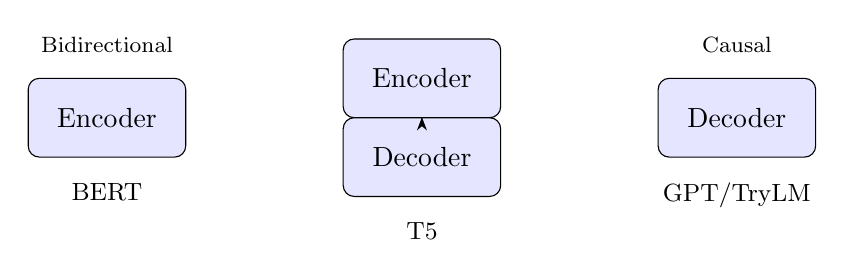
\begin{tikzpicture}[
    box/.style={rectangle, draw, rounded corners, minimum width=2cm, minimum height=1cm, fill=blue!10},
]
    % BERT
    \node[box] (bert) at (0, 0) {Encoder};
    \node[below=0.2cm of bert, font=\small] {BERT};
    \node[above=0.2cm of bert, font=\footnotesize] {Bidirectional};

    % T5
    \node[box] (t5e) at (4, 0.5) {Encoder};
    \node[box] (t5d) at (4, -0.5) {Decoder};
    \draw[-{Stealth}] (t5e) -- (t5d);
    \node[below=0.2cm of t5d, font=\small] {T5};

    % GPT
    \node[box] (gpt) at (8, 0) {Decoder};
    \node[below=0.2cm of gpt, font=\small] {GPT/TryLM};
    \node[above=0.2cm of gpt, font=\footnotesize] {Causal};
\end{tikzpicture}
\caption{Transformer architecture variants}
\end{figure}

% =============================================================================
% Appendix B: Advanced Generation Techniques
% =============================================================================
\chapter{Advanced Generation Techniques}
\label{app:advanced-generation}

This appendix covers generation methods beyond those implemented in \TryLM.

% -----------------------------------------------------------------------------
\section{Beam Search}
% -----------------------------------------------------------------------------

Instead of sampling one token at a time, beam search maintains multiple hypotheses:

\begin{algorithm}[H]
\caption{Beam Search}
\begin{algorithmic}[1]
\Require beam\_width $k$
\State beams $\gets$ [(prompt, 0.0)]  \Comment{(sequence, log\_prob)}
\For{each position}
    \State candidates $\gets$ []
    \For{each beam in beams}
        \State next\_logprobs $\gets$ model(beam.sequence)
        \State top\_k $\gets$ top-k tokens from next\_logprobs
        \For{each token in top\_k}
            \State candidates.append((beam + token, beam.score + log\_prob))
        \EndFor
    \EndFor
    \State beams $\gets$ top-k candidates by score
\EndFor
\State \Return beam with highest score
\end{algorithmic}
\end{algorithm}

\textbf{Pros}: More likely to find high-probability sequences.

\textbf{Cons}: Can be repetitive; less diverse than sampling.

% -----------------------------------------------------------------------------
\section{Contrastive Decoding}
% -----------------------------------------------------------------------------

Uses a smaller ``amateur'' model to improve a larger ``expert'' model:

\begin{equation}
\log p_{\text{final}}(x) = \log p_{\text{expert}}(x) - \alpha \log p_{\text{amateur}}(x)
\end{equation}

The idea: subtract out generic patterns that both models predict, amplifying what only the expert knows.

% -----------------------------------------------------------------------------
\section{Speculative Decoding}
% -----------------------------------------------------------------------------

Uses a small ``draft'' model to generate candidates, then verifies with the large model:

\begin{enumerate}
    \item Draft model generates $k$ tokens quickly
    \item Large model scores all $k$ tokens in one forward pass
    \item Accept tokens until first rejection
    \item Resample from large model and repeat
\end{enumerate}

\textbf{Benefit}: 2--3x speedup when draft model is accurate.

% -----------------------------------------------------------------------------
\section{Classifier-Free Guidance}
% -----------------------------------------------------------------------------

Amplifies the effect of a prompt by contrasting with unconditional generation:

\begin{equation}
\log p_{\text{guided}} = \log p_{\text{uncond}} + \gamma(\log p_{\text{cond}} - \log p_{\text{uncond}})
\end{equation}

Higher $\gamma$ makes generation more faithful to the prompt.

% -----------------------------------------------------------------------------
\section{Constrained Generation}
% -----------------------------------------------------------------------------

Force generation to satisfy constraints:

\begin{itemize}
    \item \textbf{JSON mode}: Only allow valid JSON syntax
    \item \textbf{Grammar constraints}: Follow a formal grammar
    \item \textbf{Keyword inclusion}: Ensure certain words appear
\end{itemize}

\begin{lstlisting}[style=python]
def constrained_sample(logits, allowed_tokens):
    mask = torch.full_like(logits, float("-inf"))
    mask[allowed_tokens] = 0
    return F.softmax(logits + mask, dim=-1)
\end{lstlisting}

% =============================================================================
% Appendix C: Debugging Guide
% =============================================================================
\chapter{Debugging Guide}
\label{app:debugging}

This appendix provides solutions to common issues encountered when training language models.

% -----------------------------------------------------------------------------
\section{NaN Loss}
% -----------------------------------------------------------------------------

\textbf{Symptoms}: Loss becomes \texttt{nan} or \texttt{inf} during training.

\subsection{Causes}

\begin{enumerate}
    \item \textbf{Learning rate too high}: Gradients explode
    \item \textbf{No gradient clipping}: Large gradients cause overflow
    \item \textbf{Numerical instability in attention}: $\exp$ overflow in softmax
    \item \textbf{Division by zero}: Usually in normalization layers
    \item \textbf{Bad data}: Infinite or NaN values in input
\end{enumerate}

\subsection{Solutions}

\begin{lstlisting}[style=python]
# 1. Reduce learning rate
learning_rate = 1e-4  # Instead of 3e-4

# 2. Enable gradient clipping
torch.nn.utils.clip_grad_norm_(model.parameters(), max_norm=1.0)

# 3. Check for NaN in gradients
for name, param in model.named_parameters():
    if param.grad is not None and torch.isnan(param.grad).any():
        print(f"NaN gradient in {name}")

# 4. Check data for NaN
assert not torch.isnan(input_ids).any(), "NaN in input"

# 5. Add epsilon to divisions
rms = torch.sqrt(torch.mean(x ** 2, dim=-1, keepdim=True) + 1e-6)
\end{lstlisting}

\subsection{Debugging Script}

\begin{lstlisting}[style=python]
def check_model_health(model, batch):
    """Check for numerical issues."""
    model.eval()
    with torch.no_grad():
        output = model(**batch)

        # Check loss
        if torch.isnan(output["loss"]) or torch.isinf(output["loss"]):
            print("WARNING: Loss is NaN or Inf")

        # Check logits
        logits = output["logits"]
        print(f"Logits - min: {logits.min():.2f}, max: {logits.max():.2f}")

        if torch.isnan(logits).any():
            print("WARNING: NaN in logits")

        # Check for extreme values
        if logits.abs().max() > 100:
            print("WARNING: Extreme logit values")
\end{lstlisting}

% -----------------------------------------------------------------------------
\section{Loss Not Decreasing}
% -----------------------------------------------------------------------------

\textbf{Symptoms}: Loss stays flat or decreases very slowly.

\subsection{Causes and Solutions}

\begin{enumerate}
    \item \textbf{Learning rate too low}:
    \begin{lstlisting}[style=python]
# Try increasing learning rate
learning_rate = 1e-3  # Instead of 1e-4
    \end{lstlisting}

    \item \textbf{Bug in data pipeline}:
    \begin{lstlisting}[style=python]
# Verify data looks correct
batch = next(iter(train_loader))
print(tokenizer.decode(batch["input_ids"][0]))
print(f"Labels: {batch['labels'][0][:20]}")
    \end{lstlisting}

    \item \textbf{Labels not shifted correctly}:
    \begin{lstlisting}[style=python]
# Correct shift operation
input_ids = tokens[:-1]
labels = tokens[1:]
    \end{lstlisting}

    \item \textbf{Model too small}:
    \begin{lstlisting}[style=python]
# Increase capacity
config = ModelConfig(
    n_layers=8,    # Was 6
    d_model=512,   # Was 384
)
    \end{lstlisting}

    \item \textbf{Optimizer not updating}:
    \begin{lstlisting}[style=python]
# Ensure backward and step are called
loss.backward()
optimizer.step()
optimizer.zero_grad()  # Don't forget this!
    \end{lstlisting}
\end{enumerate}

% -----------------------------------------------------------------------------
\section{Out of Memory (OOM)}
% -----------------------------------------------------------------------------

\textbf{Symptoms}: \texttt{CUDA out of memory} error.

\subsection{Solutions}

\begin{enumerate}
    \item \textbf{Reduce batch size}:
    \begin{lstlisting}[style=python]
batch_size = 32  # Instead of 64
    \end{lstlisting}

    \item \textbf{Use gradient accumulation}:
    \begin{lstlisting}[style=python]
# Effective batch = 64, actual batch = 16
accumulation_steps = 4
batch_size = 16

for i, batch in enumerate(train_loader):
    loss = model(**batch)["loss"] / accumulation_steps
    loss.backward()

    if (i + 1) % accumulation_steps == 0:
        optimizer.step()
        optimizer.zero_grad()
    \end{lstlisting}

    \item \textbf{Reduce context length}:
    \begin{lstlisting}[style=python]
context_length = 256  # Instead of 512
    \end{lstlisting}

    \item \textbf{Enable mixed precision}:
    \begin{lstlisting}[style=python]
scaler = torch.cuda.amp.GradScaler()
with torch.cuda.amp.autocast():
    loss = model(**batch)["loss"]
    \end{lstlisting}

    \item \textbf{Clear cache}:
    \begin{lstlisting}[style=python]
torch.cuda.empty_cache()
    \end{lstlisting}
\end{enumerate}

\subsection{Memory Estimation}

\begin{equation}
\text{Memory} \approx 4 \times N + B \times L^2 \times H
\end{equation}

where:
\begin{itemize}
    \item $N$ = parameters (in float32 = 4 bytes each)
    \item $B$ = batch size
    \item $L$ = sequence length
    \item $H$ = number of heads (for attention matrices)
\end{itemize}

% -----------------------------------------------------------------------------
\section{Overfitting}
% -----------------------------------------------------------------------------

\textbf{Symptoms}: Training loss decreases but validation loss increases.

\subsection{Solutions}

\begin{enumerate}
    \item \textbf{Add dropout}:
    \begin{lstlisting}[style=python]
config = ModelConfig(dropout=0.2)  # Was 0.1
    \end{lstlisting}

    \item \textbf{Use more data}: TinyStories has 2.1M stories; ensure you're using all of it.

    \item \textbf{Reduce model size}:
    \begin{lstlisting}[style=python]
config = ModelConfig(
    n_layers=4,    # Was 6
    d_model=256,   # Was 384
)
    \end{lstlisting}

    \item \textbf{Add weight decay}:
    \begin{lstlisting}[style=python]
optimizer = AdamW(model.parameters(), weight_decay=0.1)
    \end{lstlisting}

    \item \textbf{Early stopping}:
    \begin{lstlisting}[style=python]
if val_loss > best_val_loss:
    patience_counter += 1
    if patience_counter >= patience:
        print("Early stopping!")
        break
    \end{lstlisting}
\end{enumerate}

% -----------------------------------------------------------------------------
\section{Repetitive Generation}
% -----------------------------------------------------------------------------

\textbf{Symptoms}: Model generates the same words or phrases repeatedly.

\subsection{Solutions}

\begin{enumerate}
    \item \textbf{Increase temperature}:
    \begin{lstlisting}[style=python]
temperature = 1.0  # Instead of 0.7
    \end{lstlisting}

    \item \textbf{Use repetition penalty}:
    \begin{lstlisting}[style=python]
def apply_repetition_penalty(logits, generated, penalty=1.2):
    for token in set(generated):
        logits[token] /= penalty
    return logits
    \end{lstlisting}

    \item \textbf{Use top-p sampling}:
    \begin{lstlisting}[style=python]
top_p = 0.9  # Nucleus sampling
    \end{lstlisting}

    \item \textbf{Train longer}: Model may not have learned enough diversity.
\end{enumerate}

% -----------------------------------------------------------------------------
\section{Slow Training}
% -----------------------------------------------------------------------------

\textbf{Symptoms}: Training takes longer than expected.

\subsection{Solutions}

\begin{enumerate}
    \item \textbf{Use torch.compile}:
    \begin{lstlisting}[style=python]
model = torch.compile(model)  # 1.5-2x speedup
    \end{lstlisting}

    \item \textbf{Enable mixed precision}:
    \begin{lstlisting}[style=python]
with torch.cuda.amp.autocast():
    loss = model(**batch)["loss"]
    \end{lstlisting}

    \item \textbf{Increase batch size}: Larger batches use GPU more efficiently.

    \item \textbf{Use multiple workers}:
    \begin{lstlisting}[style=python]
DataLoader(dataset, num_workers=4, pin_memory=True)
    \end{lstlisting}

    \item \textbf{Profile your code}:
    \begin{lstlisting}[style=python]
with torch.profiler.profile() as prof:
    model(**batch)
print(prof.key_averages().table())
    \end{lstlisting}
\end{enumerate}

% -----------------------------------------------------------------------------
\section{Debugging Checklist}
% -----------------------------------------------------------------------------

\begin{enumerate}
    \item[$\square$] Data loads correctly (decode and inspect samples)
    \item[$\square$] Labels are shifted by one position
    \item[$\square$] Attention mask matches padding
    \item[$\square$] Model parameters are on correct device
    \item[$\square$] Optimizer is updating parameters
    \item[$\square$] Learning rate schedule is correct
    \item[$\square$] Gradient clipping is enabled
    \item[$\square$] Loss is decreasing (not flat or NaN)
    \item[$\square$] Validation loss is tracked
    \item[$\square$] Checkpoints are being saved
\end{enumerate}


% =============================================================================
% Appendix D: Glossary
% =============================================================================
\chapter{Glossary}
\label{app:glossary}

\begin{description}[style=nextline, leftmargin=2cm]

\item[Attention]
Mechanism that allows each token to ``look at'' other tokens in the sequence. Computes weighted combinations based on relevance. See Chapter~\ref{ch:self-attention}.

\item[Attention Mask]
Binary tensor indicating which positions should be attended to (1) or ignored (0). Used to prevent attending to padding tokens.

\item[Autoregressive]
Generation strategy where each token is predicted based only on previous tokens. The model generates one token at a time, feeding each output back as input.

\item[Batch Size]
Number of training examples processed together in one forward/backward pass. Larger batches provide more stable gradients but require more memory.

\item[BOS (Beginning of Sequence)]
Special token marking the start of a sequence. In \TryLM: \texttt{<|bos|>}.

\item[BPE (Byte Pair Encoding)]
Tokenization algorithm that iteratively merges the most frequent character pairs. Creates a vocabulary of subword units.

\item[Causal Masking]
Attention pattern where each position can only attend to earlier positions. Prevents the model from ``seeing the future'' during training.

\item[Checkpoint]
Saved state of a model during training, including weights, optimizer state, and configuration. Enables resuming training and inference.

\item[Context Length]
Maximum sequence length the model can process. \TryLM uses 512 tokens.

\item[Cross-Entropy Loss]
Loss function measuring the difference between predicted probability distribution and true labels. Standard loss for classification tasks including language modeling.

\item[d\_model]
Dimension of token embeddings and hidden states throughout the model. \TryLM uses 384.

\item[Decoder-Only]
Transformer architecture using only the decoder portion with causal masking. Used for text generation (GPT-style). Contrasts with encoder-only (BERT) or encoder-decoder (T5).

\item[Dropout]
Regularization technique that randomly sets activations to zero during training. Prevents overfitting.

\item[Embedding]
Dense vector representation of a discrete token. Maps vocabulary indices to continuous vectors.

\item[EOS (End of Sequence)]
Special token marking the end of a sequence. Signals generation should stop. In \TryLM: \texttt{<|eos|>}.

\item[Epoch]
One complete pass through the entire training dataset.

\item[Feed-Forward Network (FFN)]
Two-layer neural network applied to each token independently. In transformers, typically expands dimension then projects back.

\item[Fine-tuning]
Training a pre-trained model on a specific task or dataset. Adapts general knowledge to specialized domains.

\item[Flash Attention]
Optimized attention implementation achieving O(n) memory instead of O(n²). Uses tiling to avoid materializing the full attention matrix.

\item[FLOPs]
Floating-point operations. Measure of computational cost. One forward+backward pass costs approximately 6N FLOPs per token, where N is parameter count.

\item[Gradient Accumulation]
Technique to simulate larger batch sizes by accumulating gradients over multiple forward passes before updating weights.

\item[Gradient Clipping]
Limiting gradient magnitude to prevent exploding gradients. Typically clip to max norm of 1.0.

\item[Head (Attention Head)]
One of multiple parallel attention computations in multi-head attention. Each head can learn different attention patterns.

\item[Hidden Size]
See d\_model.

\item[Inference]
Using a trained model to make predictions on new data. Contrast with training.

\item[KV Cache]
Stored key and value tensors from previous positions during generation. Avoids recomputing attention for already-generated tokens.

\item[Language Model]
Model that predicts probability distributions over tokens. Can be used for text generation, completion, and understanding.

\item[LayerNorm]
Normalization technique that normalizes across features for each example. Stabilizes training.

\item[Learning Rate]
Step size for optimizer updates. Controls how much weights change each step. Typical values: 1e-4 to 1e-3.

\item[Logits]
Raw (unnormalized) output scores from the model before softmax. Shape: (batch, sequence, vocab\_size).

\item[Loss]
Scalar value measuring how wrong the model's predictions are. Training minimizes this value.

\item[Mixed Precision]
Training with both float16 and float32 precision. Reduces memory and increases speed while maintaining accuracy.

\item[MoE (Mixture of Experts)]
Architecture using multiple ``expert'' FFN layers with a router selecting which experts process each token.

\item[Multi-Head Attention]
Attention mechanism with multiple parallel attention heads, each operating on a portion of the embedding dimension.

\item[Next-Token Prediction]
The core task of language models: given a sequence, predict the probability distribution over possible next tokens.

\item[Optimizer]
Algorithm that updates model weights based on gradients. AdamW is standard for transformers.

\item[Overfitting]
When a model performs well on training data but poorly on new data. Sign: training loss decreases while validation loss increases.

\item[PAD (Padding)]
Special token used to fill sequences to equal length for batching. Usually masked in attention. In \TryLM: \texttt{<|pad|>}.

\item[Parameters]
Learnable weights in the model. \TryLM has approximately 10.8M parameters.

\item[Perplexity]
Evaluation metric for language models. Exponential of cross-entropy loss: $\text{PPL} = \exp(\text{loss})$. Lower is better.

\item[Position Encoding]
Information added to embeddings indicating token position in the sequence. Can be learned, sinusoidal, or rotary (RoPE).

\item[Pre-norm]
Transformer variant where normalization is applied before (rather than after) attention and FFN layers. More stable training.

\item[Pre-training]
Initial training phase on large amounts of unlabeled text. Learns general language patterns.

\item[Query, Key, Value (Q, K, V)]
Three projections of the input used in attention. Query asks ``what am I looking for?'', Key says ``what do I contain?'', Value provides ``what information to pass.''

\item[Residual Connection]
Adding the input of a layer to its output: $x + f(x)$. Helps gradient flow and enables training deep networks.

\item[RMSNorm]
Simplified normalization using only root mean square (no mean centering). Computationally cheaper than LayerNorm.

\item[RoPE (Rotary Position Embedding)]
Position encoding that rotates query and key vectors based on position. Encodes relative positions naturally.

\item[Sampling]
Selecting the next token probabilistically from the model's output distribution. Contrast with greedy decoding.

\item[Scaling Laws]
Empirical relationships between model size, data size, compute, and performance. Chinchilla: optimal compute means N $\propto$ D.

\item[Self-Attention]
Attention where queries, keys, and values all come from the same sequence. The model attends to itself.

\item[Softmax]
Function converting logits to probabilities: $\text{softmax}(x_i) = \frac{\exp(x_i)}{\sum_j \exp(x_j)}$.

\item[Step]
One optimizer update. With gradient accumulation, may involve multiple forward passes.

\item[SwiGLU]
Gated activation function: $\text{SwiGLU}(x) = \text{Swish}(xW_g) \odot (xW_u)$. Outperforms GELU in language models.

\item[Temperature]
Scaling factor for logits before softmax. Higher temperature $\to$ more random; lower $\to$ more deterministic.

\item[Token]
Atomic unit of text for the model. Can be a word, subword, or character depending on tokenization.

\item[Tokenizer]
Algorithm converting text to token IDs and vice versa. \TryLM uses BPE with 16,384 vocabulary size.

\item[Top-k Sampling]
Sampling strategy that only considers the k most probable tokens. Filters out unlikely tokens.

\item[Top-p (Nucleus) Sampling]
Sampling from the smallest set of tokens whose cumulative probability exceeds p. Adapts to probability distribution shape.

\item[Training Loop]
The iterative process: forward pass $\to$ loss computation $\to$ backward pass $\to$ optimizer step.

\item[Transformer]
Neural network architecture based on self-attention. Foundation of modern language models.

\item[UNK (Unknown)]
Special token for out-of-vocabulary inputs. With BPE, rarely needed. In \TryLM: \texttt{<|unk|>}.

\item[Validation]
Evaluating model on held-out data during training. Used to detect overfitting and select best checkpoint.

\item[Vocabulary]
Set of all tokens the model can process. \TryLM uses 16,384 tokens.

\item[Warmup]
Gradually increasing learning rate at the start of training. Helps stability.

\item[Weight Decay]
Regularization adding penalty for large weights: $L_{\text{total}} = L + \lambda \|w\|^2$. AdamW applies this directly to weights.

\item[Weight Tying]
Sharing weights between input embeddings and output projection. Reduces parameters and improves quality.

\end{description}



% -----------------------------------------------------------------------------
% Back Matter
% -----------------------------------------------------------------------------
\backmatter

% Bibliography (if using)
% \printbibliography[heading=bibintoc]

% Index (if using)
% \printindex

% =============================================================================
\end{document}
% =============================================================================
